%==============================================================================
%  EmoLearn — Mémoire de Master
%  Fichier principal. Compiler avec : pdfLaTeX + Biber + pdfLaTeX + pdfLaTeX
%  (dans TeXstudio : choisir "PDFLaTeX" et "Biber" comme backend bibliographie)
%==============================================================================
\documentclass[12pt,a4paper,oneside]{report}

%------------------------- Encodage & langue ---------------------------------
\usepackage[utf8]{inputenc}
\usepackage[T1]{fontenc}
\usepackage{lmodern} % police type modèle LaTeX (comme l'image collée)
\usepackage[french]{babel}
\usepackage{csquotes}
\babelhyphenation{régulation}

%------------------------- Mise en page --------------------------------------
\usepackage[a4paper,top=2.5cm,bottom=2.5cm,left=3cm,right=2.5cm]{geometry}
\usepackage{setspace}
\onehalfspacing
\usepackage{parskip}
\usepackage{emptypage}

%------------------------- Graphismes & tableaux -----------------------------
\usepackage{graphicx}
\usepackage{booktabs}
\usepackage{array}
\usepackage{tabularx}
\usepackage{longtable}
\usepackage{multirow}
\usepackage{float}
\usepackage{xcolor}
\usepackage{colortbl}
\usepackage{enumitem}

%------------------------- Maths ---------------------------------------------
\usepackage{amsmath}
\usepackage{amssymb}

%------------------------- Pseudo-code ---------------------------------------
\usepackage{algorithm}
\usepackage{algpseudocode}
\floatname{algorithm}{Algorithme}
\renewcommand{\algorithmicrequire}{\textbf{Entrée :}}
\renewcommand{\algorithmicensure}{\textbf{Sortie :}}
\renewcommand{\algorithmicif}{\textbf{si}}
\renewcommand{\algorithmicthen}{\textbf{alors}}
\renewcommand{\algorithmicelse}{\textbf{sinon}}
\renewcommand{\algorithmicend}{\textbf{fin}}
\renewcommand{\algorithmicfor}{\textbf{pour}}
\renewcommand{\algorithmicdo}{\textbf{faire}}
\renewcommand{\algorithmicreturn}{\textbf{retourner}}

%------------------------- Schémas (TikZ) ------------------------------------
\usepackage{tikz}
\usetikzlibrary{arrows.meta,positioning,shapes.geometric,calc,fit,backgrounds}

%------------------------- En-têtes & pieds de page --------------------------
\usepackage{fancyhdr}
\setlength{\headheight}{15pt}
\pagestyle{fancy}
\fancyhf{}
\fancyhead[L]{\nouppercase{\leftmark}}
\fancyfoot[C]{\thepage}% numérotation en bas, au milieu
\renewcommand{\headrulewidth}{0.4pt}
\renewcommand{\footrulewidth}{0pt}
% Pages de chapitre / liminaires : numéro seul, en bas au centre
\fancypagestyle{plain}{%
  \fancyhf{}%
  \fancyfoot[C]{\thepage}%
  \renewcommand{\headrulewidth}{0pt}%
  \renewcommand{\footrulewidth}{0pt}%
}
% S'assurer que le style plain (numéro au milieu) est utilisé partout où besoin
\makeatletter
\let\ps@chapter\ps@plain
\makeatother

%------------------------- Titres de chapitres (style Lenny) ------------------
\usepackage[Lenny]{fncychap}

%------------------------- Mini-sommaires de chapitre -------------------------
\usepackage[french,nolistfiles,nohints]{minitoc}
\setcounter{minitocdepth}{2}

% Page de titre + Sommaire (sections et sous-sections), contenu à la page suivante.
\newcommand{\titreduchapitre}[2]{%
  \chapter{\textbf{#1}}%
  \label{#2}%
  \minitoc
  \thispagestyle{plain}% numéro de page en bas au centre
  \newpage
  \thispagestyle{fancy}}

%------------------------- Liens & références ---------------------------------
\usepackage{hyperref}
\hypersetup{
  colorlinks=true,
  linkcolor=black,
  citecolor=blue!50!black,
  urlcolor=blue!50!black,
  pdftitle={EmoLearn — Mémoire de Master},
  pdfauthor={BRIKI Maram}
}

%------------------------- Bibliographie (biblatex + biber) -------------------
\usepackage[backend=biber,style=numeric-comp,sorting=nyt,maxbibnames=99]{biblatex}
\addbibresource{references.bib}

%------------------------- Raccourcis ----------------------------------------
\newcommand{\emolearn}{\textsc{EmoLearn}}

% Marqueur des parties non encore rédigées. Il évite aussi les pages blanches
% que produisent de longues suites de titres sans texte intercalé.
% Pour faire disparaître tous les marqueurs d'un coup :
%   \renewcommand{\arediger}{}
\newcommand{\arediger}{\par\nobreak\vspace{2pt}%
  \emph{\small[Contenu à rédiger.]}\par\medskip}

%==============================================================================
\begin{document}
\dominitoc

%--------------------------- PAGE DE GARDE ------------------------------------
%==============================================================================
%  PAGE DE GARDE — ESCT à gauche, ISAMM à droite
%  Logos : logo_esct.png | logo_isamm.png
%==============================================================================
\definecolor{titrebleu}{RGB}{0,0,90}

\begin{titlepage}
\thispagestyle{empty}
\newgeometry{top=1.5cm,bottom=1.8cm,left=2cm,right=2cm}
\setlength{\parskip}{0pt}
\centering
\renewcommand{\rmdefault}{lmr}%
\normalfont\rmfamily

%------------------------- En-tête : ESCT | texte | ISAMM --------------------
\noindent
\begin{minipage}[c]{0.23\textwidth}
\centering

\includegraphics[width=2.35cm,keepaspectratio]{logos/logo_esct.png}%
\end{minipage}%
\hfill
\begin{minipage}[c]{0.52\textwidth}
\centering
{\normalsize \textbf{République Tunisienne}\par}
\vspace{1pt}
{\footnotesize \textbf{Ministère de l'Enseignement Supérieur\\
et de la Recherche Scientifique}\par}
\vspace{3pt}
{\normalsize \textbf{Université de La Manouba}\par}
\vspace{1pt}
{\normalsize \textbf{École Supérieure de Commerce de Tunis}\par}
\vspace{1pt}
{\footnotesize \textbf{Institut Supérieur des Arts Multimédia\\
de la Manouba}\par}
\end{minipage}%
\hfill
\begin{minipage}[c]{0.23\textwidth}
\centering

\includegraphics[width=2.35cm,keepaspectratio]{logos/logo_isamm.png}%
\end{minipage}

\vspace{1.8cm}

%------------------------- Type de diplôme -----------------------------------
{\Large MÉMOIRE DE MASTER DE RECHERCHE\par}
\vspace{0.55cm}
{\normalsize \textbf{Présenté en vue de l'obtention du}\par}
\vspace{0.28cm}
{\normalsize MASTER DE RECHERCHE EN INFORMATIQUE\\[2pt]
DÉCISIONNELLE ET INTELLIGENTE APPLIQUÉE À LA GESTION\par}
\vspace{0.4cm}
{\normalsize \textbf{Parcours :} Aide à la Décision\par}

\vspace{1.3cm}

%------------------------- Titre (bleu, entre filets) ------------------------
\rule{\textwidth}{1.7pt}\\[0.55cm]
{\large\bfseries\color{titrebleu}%
Vers une approche de personnalisation pédagogique adaptative\\[0.25cm]
basée sur la détection multimodale d'états émotionnels\\[0.25cm]
et l'IA générative\par}
\vspace{0.5cm}
\rule{\textwidth}{1.5pt}

\vspace{1.4cm}

%------------------------- Auteur --------------------------------------------
{\large \textit{Par}\par}
\vspace{0.3cm}
{\Large Briki Maram\par}

\vspace{1.15cm}

%------------------------- Encadrante ----------------------------------------
{\normalsize \textbf{Encadrante académique :} Dr. REZGUI Kalthoum, \textit{ISAMM}\par}

\vfill

%------------------------- Année ---------------------------------------------
{\normalsize Année Universitaire : 2025 -- 2026\par}

\restoregeometry
\end{titlepage}


%--------------------------- PAGES LIMINAIRES ---------------------------------
\pagenumbering{roman}

%==============================================================================
%  DÉDICACE — paragraphe centré, chapeau (sans décor floral)
%==============================================================================
\chapter*{}
\thispagestyle{plain}
\vspace*{-2.3cm}
\singlespacing
\setlength{\parskip}{0.55em}

\begin{center}
\begin{tikzpicture}[x=0.92cm,y=0.92cm]
  \fill[black!42] (-0.46,0.42) -- (-0.52,1.28) -- (0.52,1.28) -- (0.46,0.42)
    -- cycle;
  \fill[black!58] (0,1.28) -- (1.48,1.82) -- (0,2.36) -- (-1.48,1.82) -- cycle;
  \fill[black!72] (0,1.82) circle (0.07);
  \draw[black!55, line width=0.75pt] (0,1.82) -- (1.22,1.48);
  \fill[black!55] (1.22,1.26) -- (1.36,1.50) -- (1.08,1.50) -- cycle;
\end{tikzpicture}

\vspace{0.12cm}
{\LARGE\bfseries Dédicace\par}
\vspace{0.18cm}
\includegraphics[height=0.85cm]{logos/phrase_arabe_dedicace.png}
\end{center}

\vspace{0.7cm}

\begin{center}
Je dédie ce travail à tous ceux qui m'ont appris à aimer le savoir\\
et qui m'ont aidée dans mon apprentissage.

\vspace{0.35cm}

À ma mère, \textbf{Radhia}, et à mon père, \textbf{Dhahbi},\\
pour leur amour, leurs prières et leur soutien constant,

À ma tante, \textbf{Jalila}, pour sa bienveillance et ses conseils,

À mes frères, \textbf{Hosni} et \textbf{Amara}, pour leur solidarité,

À toute ma famille pour leur soutien.

\vspace{0.35cm}

À mon partenaire, \textbf{Aymen}, pour sa patience et son appui,

À mes amis, merci pour leur soutien.

\vspace{0.35cm}

Et à tous ceux qui ont aidé, d'une manière ou d'une autre,\\
à atteindre ce succès,\\
je vous exprime ma profonde gratitude et mon respect.
\end{center}

\vspace{1.1cm}
\begin{flushright}
\textit{Maram Briki}
\end{flushright}

\onehalfspacing
\setlength{\parskip}{0.5em plus 0.1em minus 0.1em}

%==============================================================================
%  REMERCIEMENTS — modèle centré (comme l'image collée)
%==============================================================================
\chapter*{\textbf{Remerciements}}
\addcontentsline{toc}{chapter}{Remerciements}
\mtcaddchapter % aligne le compteur minitoc avec la TOC (pas de Sommaire ici)
\thispagestyle{plain}
\singlespacing

\vspace*{1.2cm}

\begin{center}
\textbf{ À mon encadrante}\\[0.35cm]
\textbf{Dr. REZGUI Kalthom}
\end{center}

\vspace{1.4cm}

\begin{center}
Je tiens à exprimer ma profonde gratitude pour avoir accepté\\
d'encadrer ce travail de recherche.
\end{center}

\vspace{0.85cm}

\begin{center}
Je vous remercie sincèrement pour le temps que vous y avez consacré\\
ainsi que pour votre soutien tout au long de ce projet.
\end{center}

\vspace{0.85cm}

\begin{center}
Je vous suis reconnaissante pour les ressources mises à ma disposition\\
et pour l'encadrement de qualité dont j'ai bénéficié.
\end{center}

\vspace{0.85cm}

\begin{center}
Votre patience, votre professionnalisme, vos conseils et vos remarques\\
constructives ont contribué de manière significative à la réussite\\
de ce travail.
\end{center}

\vspace{0.85cm}

\begin{center}
Enfin, j'adresse mes sincères remerciements aux membres du jury\\
pour leur temps et leur évaluation attentive.
\end{center}

\onehalfspacing


\cleardoublepage
\renewcommand{\contentsname}{\textbf{Table des matières}}
\tableofcontents

\cleardoublepage
\phantomsection
\addcontentsline{toc}{chapter}{Table des figures}
\mtcaddchapter % entrée TOC sans \chapter numéroté : resync minitoc
\renewcommand{\listfigurename}{\textbf{Table des figures}}
\listoffigures

\cleardoublepage
\phantomsection
\addcontentsline{toc}{chapter}{Liste des tableaux}
\mtcaddchapter % entrée TOC sans \chapter numéroté : resync minitoc
\renewcommand{\listtablename}{\textbf{Liste des tableaux}}
\listoftables

%--------------------------- CORPS DU MÉMOIRE ---------------------------------
\cleardoublepage
\pagenumbering{arabic}

%==============================================================================
%  INTRODUCTION GÉNÉRALE — non numérotée (avant le chapitre 1)
%==============================================================================
\chapter*{\textbf{Introduction générale}}
\addcontentsline{toc}{chapter}{Introduction générale}
\mtcaddchapter % aligne le compteur minitoc (pas de Sommaire sur l'intro)
\label{chap:introduction}
\markboth{Introduction générale}{Introduction générale}
\thispagestyle{plain}

L'évolution rapide des technologies numériques et le développement des
plateformes éducatives en ligne ont profondément transformé les pratiques
d'apprentissage, en particulier à travers la diffusion des cours en ligne
ouverts et massifs (MOOC, \emph{Massive Open Online Courses}). Ces dispositifs
permettent aujourd'hui de collecter, diffuser et personnaliser des contenus
pédagogiques à grande échelle, offrant à des millions d'apprenants un accès
élargi à la formation, indépendamment des contraintes géographiques
\cite{breslow2013studying,daniel2012making}. La crise sanitaire de 2020 a
encore accéléré cette dynamique, faisant de l'apprentissage en ligne une
composante désormais structurelle des systèmes éducatifs contemporains.

Toutefois, cette évolution s'accompagne d'un constat largement documenté :
les MOOC souffrent de taux d'abandon particulièrement élevés. Une part
importante des inscrits interrompt son parcours dès les premières semaines,
ce qui limite fortement l'efficacité pédagogique réelle de ces dispositifs
\cite{onah2014dropout,jordan2015massive}. Parmi les facteurs explicatifs,
la baisse de l'\textbf{engagement} de l'apprenant occupe une place centrale
\cite{kizilcec2013deconstructing,hew2016promoting}. Dans une salle de classe
traditionnelle, l'enseignant perçoit en permanence des signaux fins (regard,
posture, expression) et adapte spontanément son discours. Cette boucle de
régulation disparaît presque entièrement dans les environnements en ligne de
masse, où l'apprenant fait face à un contenu figé, identique pour tous et
insensible à son état du moment.

Dans ce contexte, plusieurs travaux en informatique affective et en
psychologie de l'apprentissage ont établi que les émotions ne sont pas
périphériques à la cognition, mais en constituent un rouage essentiel
\cite{picard1997affective,pekrun2006control}. Des états tels que l'ennui, la
confusion ou la frustration influencent directement la profondeur du traitement
de l'information, la persévérance et la mémorisation
\cite{dmello2012dynamics,baker2010better}. Une détection inefficace de ces
états, combinée à l'absence d'adaptation pédagogique, peut entraîner une
dégradation de l'expérience d'apprentissage et favoriser le décrochage. Cette
problématique est d'autant plus critique que les décisions pédagogiques doivent
idéalement intervenir en temps utile, avant que le désengagement ne s'installe.

Ainsi, ce mémoire s'inscrit dans cette problématique en proposant une approche
visant à réunir, au sein d'une même chaîne de traitement, la perception de
l'engagement émotionnel et la génération adaptative de contenu pédagogique.

Face à ces enjeux, la question centrale de ce travail est la suivante :

\begin{center}
\textit{Comment concevoir un dispositif capable d'inférer automatiquement
l'état d'engagement d'un apprenant à partir de signaux multimodaux, puis de
générer en réponse un contenu pédagogique adapté à cet état, tout en
garantissant la cohérence et la traçabilité de la décision pédagogique
sous-jacente~?}
\end{center}

Cette question se décompose en quatre sous-questions opérationnelles :

\begin{itemize}
  \item Comment estimer de manière fiable l'état d'engagement à partir de
  signaux multimodaux hétérogènes (expressions faciales issues de
  \textsc{DAiSEE}, signal vocal issu de \textsc{IEMOCAP}), et quel gain la
  fusion apporte-t-elle par rapport à une modalité unique~?

  \item Comment formaliser une correspondance pédagogiquement justifiable
  entre les états d'engagement détectés et les stratégies d'intervention,
  c'est-à-dire un modèle \emph{engagement\,$\rightarrow$\,adaptation}~?

  \item Dans quelle mesure un grand modèle de langue, guidé par des patrons
  de prompts structurés et ancré par un mécanisme de récupération augmentée
  (RAG), peut-il produire un contenu pédagogique pertinent et adapté à l'état
  d'engagement visé~?

  \item Selon quel protocole peut-on évaluer, de façon honnête et
  multi-niveaux, la qualité de la perception, la pertinence de la décision et
  la qualité du contenu généré~?
\end{itemize}

L'analyse de la littérature montre que, malgré les progrès importants réalisés
dans les domaines de la détection de l'engagement et de l'IA générative
appliquée à l'éducation, ces deux axes restent majoritairement traités de
manière indépendante. D'une part, les modèles de perception multimodale
permettent d'inférer l'état affectif d'un apprenant avec une fiabilité
croissante \cite{dmello2015review,whitehill2014faces,gupta2016daisee}.
D'autre part, les grands modèles de langue ouvrent la voie à une génération
de contenu pédagogique personnalisée à grande échelle
\cite{brown2020language,kasneci2023chatgpt}. Cependant, ces approches
demeurent souvent séquentielles ou fragmentées~: la détection n'est pas
systématiquement reliée à une décision pédagogique explicite, tandis que la
génération n'est pas toujours conditionnée par un état d'engagement mesuré,
ce qui limite la capacité des systèmes à restaurer une forme de régulation
pédagogique automatique.

Pour répondre à ces limitations, ce mémoire propose un framework hybride nommé
\emolearn{}, combinant trois briques complémentaires. La couche de
\textbf{perception} estime l'état d'engagement à partir de signaux visage et
voix, en s'appuyant sur les corpus \textsc{DAiSEE} et \textsc{IEMOCAP} et sur
des modèles \emph{fine-tunés} vers la taxonomie des quatre états
d'engagement~: un Vision Transformer (ViT) pour le visage et un modèle
wav2vec2 pour la voix, combinés par un moteur de fusion multimodale. La couche
de \textbf{décision} formalise un modèle
\emph{engagement\,$\rightarrow$\,adaptation} reliant chaque état à un type de
contenu et à un patron de génération. Enfin, la couche de \textbf{génération}
produit un contenu pédagogique adaptatif au moyen d'un grand modèle de langue,
guidé par une bibliothèque de vingt patrons structurés et ancré par un module
RAG sur une base documentaire pédagogique. Ainsi, \emolearn{} vise à passer
d'un contenu figé à une adaptation réellement conditionnée par l'état
d'engagement détecté.

En résumé, le module de perception anticipe l'état émotionnel de l'apprenant,
tandis que les modules de décision et de génération exploitent cette estimation
pour produire une intervention pédagogique ciblée, traçable et reproductible.

Les principales contributions de ce travail sont les suivantes :

\begin{enumerate}
  \item Proposition d'une architecture multimodale de bout en bout reliant
  perception, décision et génération au sein d'une même chaîne.

  \item Formalisation d'un modèle \emph{engagement\,$\rightarrow$\,adaptation}
  assorti d'une bibliothèque de vingt patrons de génération structurés.

  \item Développement d'un module RAG pédagogique ancrant la génération sur
  une base documentaire vectorisée.

  \item Fine-tuning supervisé des modèles de perception (ViT pour le visage et
  wav2vec2 pour la voix) vers les quatre états d'engagement \textsc{DAiSEE}.

  \item Évaluation honnête et instrumentée de la fusion multimodale, incluant
  l'analyse des compromis entre exactitude globale et sensibilité aux états
  critiques.

  \item Prototype logiciel complet et reproductible, accompagné d'un protocole
  d'évaluation multi-niveaux.
\end{enumerate}

%==============================================================================
\section*{Méthodologie générale}
\label{sec:methodologie}

La démarche adoptée relève de la \emph{recherche orientée conception}
(\emph{design science research}), paradigme particulièrement adapté à la
conception d'artefacts informatiques répondant à un problème identifié
\cite{hevner2004design}. Elle articule l'analyse d'un problème réel (le
décrochage lié à la baisse d'engagement dans les MOOC), la construction
d'un artefact (le framework \emolearn{}) et son évaluation au regard
d'objectifs explicites.

Concrètement, le travail s'organise autour d'une chaîne de traitement en trois
étages : un étage de \emph{perception} (FER, SER, fusion), un étage de
\emph{décision} (règles temporelles et moteur pédagogique) et un étage de
\emph{génération} (RAG et LLM).

Le projet s'appuie sur deux corpus publics de référence. \textsc{DAiSEE}
\cite{gupta2016daisee} constitue le socle engagement (taxonomie et scénarios),
tandis qu'\textsc{IEMOCAP} \cite{busso2008iemocap} apporte la modalité vocale
et, via un sous-corpus audiovisuel aligné, le support de validation de la
fusion. Le prototype repose sur une architecture client-serveur, des modèles
de perception fine-tunés (ViT et wav2vec2) vers les quatre états
\textsc{DAiSEE}, un LLM accessible par API et un module RAG (ChromaDB).

%==============================================================================
\section*{Structure du mémoire}
\label{sec:structure}

Le présent mémoire s'ouvre par la présente \textbf{introduction générale},
puis s'organise en six chapitres numérotés.

Le \textbf{chapitre~1} pose les fondements conceptuels de l'apprentissage
adaptatif et de l'engagement (MOOC, émotions, détection multimodale, IA
générative).

Le \textbf{chapitre~2} propose un état de l'art critique et positionne
\emolearn{} par rapport aux travaux existants.

Le \textbf{chapitre~3} est consacré à la modélisation et à la conception du
framework : architecture globale, modèle
\emph{engagement\,$\rightarrow$\,adaptation}, génération fondée sur des patrons
et un module RAG, ainsi que conception du prototype.

Le \textbf{chapitre~4} décrit l'implémentation technique de bout en bout.

Le \textbf{chapitre~5} expose la validation et les résultats selon un protocole
multi-niveaux.

Le \textbf{chapitre~6}, enfin, synthétise les contributions, expose les limites
et trace des perspectives.

Le mémoire se termine par la bibliographie.

%==============================================================================
%  CHAPITRE 1 — FONDEMENTS
%==============================================================================
\titreduchapitre{Fondements de l'apprentissage adaptatif et de l'engagement}{chap:fondements}

%==============================================================================
\section{Introduction}
\label{sec:fond-intro}

La conception d'un système d'apprentissage adaptatif fondé sur
l'engagement émotionnel mobilise un ensemble de notions issues de
domaines distincts : sciences de l'éducation, informatique affective,
apprentissage multimodal et intelligence artificielle générative. Ces
notions sont souvent présentées séparément ; les rassembler permet
d'établir un vocabulaire partagé et d'expliciter les hypothèses sur
lesquelles repose le pipeline \emolearn{}.

Ce chapitre examine les concepts fondamentaux nécessaires à la
compréhension de cette architecture. Il aborde successivement
l'apprentissage en ligne et les MOOC, la notion d'engagement de
l'apprenant, les apports de l'informatique affective, les principes de
la détection multimodale, puis les bases de l'intelligence artificielle
générative appliquée à l'éducation (LLM, guidage par prompts et RAG).

%==============================================================================
\section{Apprentissage en ligne et MOOC}
\label{sec:fond-mooc}

\subsection{Définition}

Les cours en ligne ouverts et massifs (MOOC, \emph{Massive Open Online
Courses}) désignent des dispositifs de formation accessibles à distance, le
plus souvent sans prérequis d'inscription stricts, et destinés à un public
potentiellement très large \cite{daniel2012making,breslow2013studying}. Ils
reposent typiquement sur des vidéos pédagogiques, des quiz, des forums et un
parcours de progression asynchrone.

\subsection{Implication pour l'adaptation}

Dans ce modèle, le contenu est principalement diffusé de manière uniforme.
Toute forme d'adaptation automatique suppose donc, en amont, de disposer
d'une mesure d'engagement plus fine que les simples proxies de présence
(connexion, clics), point développé dans la section suivante.

%==============================================================================
\section{Engagement de l'apprenant}
\label{sec:fond-engagement}

\subsection{Définition}

L'engagement désigne la mobilisation cognitive, comportementale et
émotionnelle de l'apprenant vis-à-vis de la tâche d'apprentissage
\cite{kizilcec2013deconstructing,hew2016promoting,fredricks2004school}. Il ne se réduit pas à la
simple présence en ligne (connexion, clics), mais renvoie à une implication
active dans le traitement de l'information.

\subsection{Dimensions de l'engagement}

On distingue classiquement :


\begin{figure}[H]
\centering
\begin{tikzpicture}[
  box/.style={rectangle, rounded corners=3pt, draw=#1, thick, fill=#1!12,
              minimum width=3.6cm, minimum height=1.55cm, align=center,
              font=\small},
  arr/.style={-{Stealth[length=2.4mm]}, thick, gray!70}
]
\node[box=teal!70!black] (cog) {\textbf{Cognitif}\\profondeur du traitement\\stratégies d'apprentissage};
\node[box=blue!70!black, right=0.55cm of cog] (beh) {\textbf{Comportemental}\\participation\\persévérance};
\node[box=orange!80!black, right=0.55cm of beh] (emo) {\textbf{Émotionnel}\\intérêt, ennui,\\frustration, etc.};
\node[draw=gray!55, dashed, rounded corners=4pt, fit=(cog)(beh)(emo),
      inner sep=8pt, label={[font=\small\bfseries]above:Engagement de l'apprenant}] {};
\node[below=0.35cm of emo, font=\footnotesize\itshape, text=orange!80!black, align=center]
  {Focus \emolearn{}};
\end{tikzpicture}
\caption{Les trois dimensions classiques de l'engagement. }
\label{fig:fond-dimensions-engagement}
\end{figure}

\emolearn{} se concentre principalement sur la dimension émotionnelle /
affective, tout en visant un effet sur la persévérance globale.

\subsection{Mesure de l'engagement}

Les indicateurs usuels en e-learning (durée de session, progression, scores)
fournissent des \emph{proxies} utiles mais incomplets. Les approches plus
récentes mobilisent des signaux multimodaux (visage, voix, posture) pour
estimer l'état affectif de manière plus directe
\cite{dmello2015review,sharma2020multimodal,goldberg2021attentive}.

%==============================================================================
\section{Informatique affective et émotions en apprentissage}
\label{sec:fond-affect}

\subsection{Rôle des émotions dans l'apprentissage}

Les travaux en psychologie de l'apprentissage montrent que les émotions
modulent l'attention, la mémorisation et la persévérance
\cite{pekrun2006control,dmello2012dynamics,baker2010better,loderer2020beyond,graesser2020emotions}. Elles ne sont
donc pas périphériques à la cognition, mais constitutives du processus
d'apprentissage.

\subsection{États pertinents pour l'adaptation pédagogique}

Dans le cadre de ce mémoire, quatre états issus du corpus \textsc{DAiSEE}
\cite{gupta2016daisee} structurent la taxonomie d'engagement :


\begin{figure}[H]
\centering
\begin{tikzpicture}[
  etat/.style={rectangle, rounded corners=3pt, draw=#1, very thick, fill=#1!14,
               minimum width=3.5cm, minimum height=1.7cm, align=center, font=\small},
  arr/.style={-{Stealth[length=2.4mm]}, thick, gray!65}
]
\node[etat=green!55!black] (eng) {\textbf{Engagement}\\implication positive\\maintenir / enrichir};
\node[etat=gray!70!black, right=0.7cm of eng] (bor) {\textbf{Ennui}\\sous-stimulation\\relancer};
\node[etat=blue!65!black, below=0.65cm of eng] (con) {\textbf{Confusion}\\incompréhension\\clarifier};
\node[etat=red!65!black, right=0.7cm of con] (fru) {\textbf{Frustration}\\blocage\\soutenir / simplifier};
\node[draw=black!40, rounded corners=5pt, fit=(eng)(bor)(con)(fru),
      inner sep=10pt,
      label={[font=\small\bfseries]above:Taxonomie \textsc{DAiSEE} (4 états)}] {};
\end{tikzpicture}
\caption{Taxonomie des quatre états d'engagement retenus (\textsc{DAiSEE}).}
\label{fig:fond-taxonomie-daisee}
\end{figure}

Chacun de ces états appelle une stratégie pédagogique distincte.

\subsection{Charge cognitive}

La théorie de la charge cognitive rappelle qu'un contenu trop dense ou mal
séquencé favorise la confusion et l'abandon
\cite{sweller1988cognitive,sweller2019cognitive}. La théorie de
l'apprentissage multimédia complète ce cadre : la conception des messages
(texte, image, rythme) conditionne la charge utile
\cite{mayer2021multimedia}. L'adaptation du niveau d'explication, du rythme
et du type d'exemple constitue dès lors un levier central des systèmes
d'apprentissage adaptatifs.

%==============================================================================
\section{Détection multimodale de l'engagement}
\label{sec:fond-detection}

\subsection{Modalités exploitées}

La détection automatique de l'engagement peut s'appuyer sur :
\begin{itemize}
  \item le \textbf{visage} (expressions faciales, regard)~;
  \item la \textbf{voix} (prosodie, intensité, variations émotionnelles)~;
  \item éventuellement la posture ou des signaux physiologiques.
\end{itemize}
\emolearn{} combine les deux premières modalités, à partir de clips
vidéo et audio annotés (hors temps réel), plutôt que de traces textuelles
de forums ou de capteurs physiologiques.

\begin{figure}[H]
\centering
\begin{tikzpicture}[
  box/.style={rectangle, rounded corners=3pt, draw=black!70, thick,
              minimum width=2.5cm, minimum height=1.05cm, align=center, font=\small},
  io/.style={rectangle, rounded corners=2pt, draw=black!50, dashed,
             minimum width=2.4cm, minimum height=0.9cm, align=center, font=\footnotesize},
  arr/.style={-{Stealth[length=2.5mm]}, very thick, black!65}
]
\node[io] (vid) at (0,3.6) {Vidéo\\visage};
\node[io] (aud) at (4.2,3.6) {Audio\\voix};
\node[box, fill=blue!10] (fer) at (0,2.2) {FER};
\node[box, fill=blue!10] (ser) at (4.2,2.2) {SER};
\node[box, fill=teal!15] (fus) at (2.1,0.85) {Fusion\\multimodale};
\node[box, fill=orange!12] (etat) at (2.1,-0.55) {État\\d'engagement};
\node[box, fill=yellow!18] (adap) at (2.1,-1.95) {Adaptation\\pédagogique};

\draw[arr] (vid) -- (fer);
\draw[arr] (aud) -- (ser);
\draw[arr] (fer) -- (fus);
\draw[arr] (ser) -- (fus);
\draw[arr] (fus) -- (etat);
\draw[arr] (etat) -- (adap);
\end{tikzpicture}
\caption{Boucle conceptuelle de détection multimodale.}
\label{fig:fond-boucle-multimodale}
\end{figure}

\subsection{Corpus de référence}

Deux corpus publics fondent la chaîne de perception :
\begin{itemize}
  \item \textsc{DAiSEE} \cite{gupta2016daisee} pour l'engagement facial annoté~;
  \item \textsc{IEMOCAP} \cite{busso2008iemocap} pour l'émotion vocale et, via
  un sous-corpus audiovisuel, la validation de la fusion alignée.
\end{itemize}

\subsection{Fusion multimodale}

La fusion vise à combiner des sources hétérogènes pour obtenir une décision
plus robuste qu'une modalité seule
\cite{liang2024foundations,gandhi2023multimodal}. Elle soulève toutefois des
questions de pondération, de désaccord inter-modalités et de déséquilibre des
classes, qui seront traités dans la conception et la validation du système.

%==============================================================================
\section{IA générative pour l'éducation}
\label{sec:fond-ia}

\subsection{Grands modèles de langue}

Les grands modèles de langue (LLM, \emph{Large Language Models}) sont des
réseaux de neurones entraînés à prédire le prochain token d'une séquence à
partir d'un très grand corpus textuel
\cite{brown2020language,vaswani2017attention,wolf2020transformers,openai2023gpt4,dubey2024llama3}. Architecturée autour du
\emph{Transformer} décodeur, cette famille de modèles suit un pipeline
strictement séquentiel (figure~\ref{fig:fond-llm-arch}) : le texte d'entrée
est d'abord \emph{tokenisé} (mots ou sous-mots convertis en identifiants
numériques), puis ces identifiants passent dans une couche d'\emph{embeddings}
combinée à un encodage de position, avant d'entrer dans une pile de blocs
d'\emph{attention} et de couches \emph{feed-forward}. Une tête de langage
produit enfin la distribution sur le vocabulaire. La génération est
\emph{auto-régressive} : chaque token prédit est réinjecté pour produire le
suivant.

\begin{figure}[H]
\centering
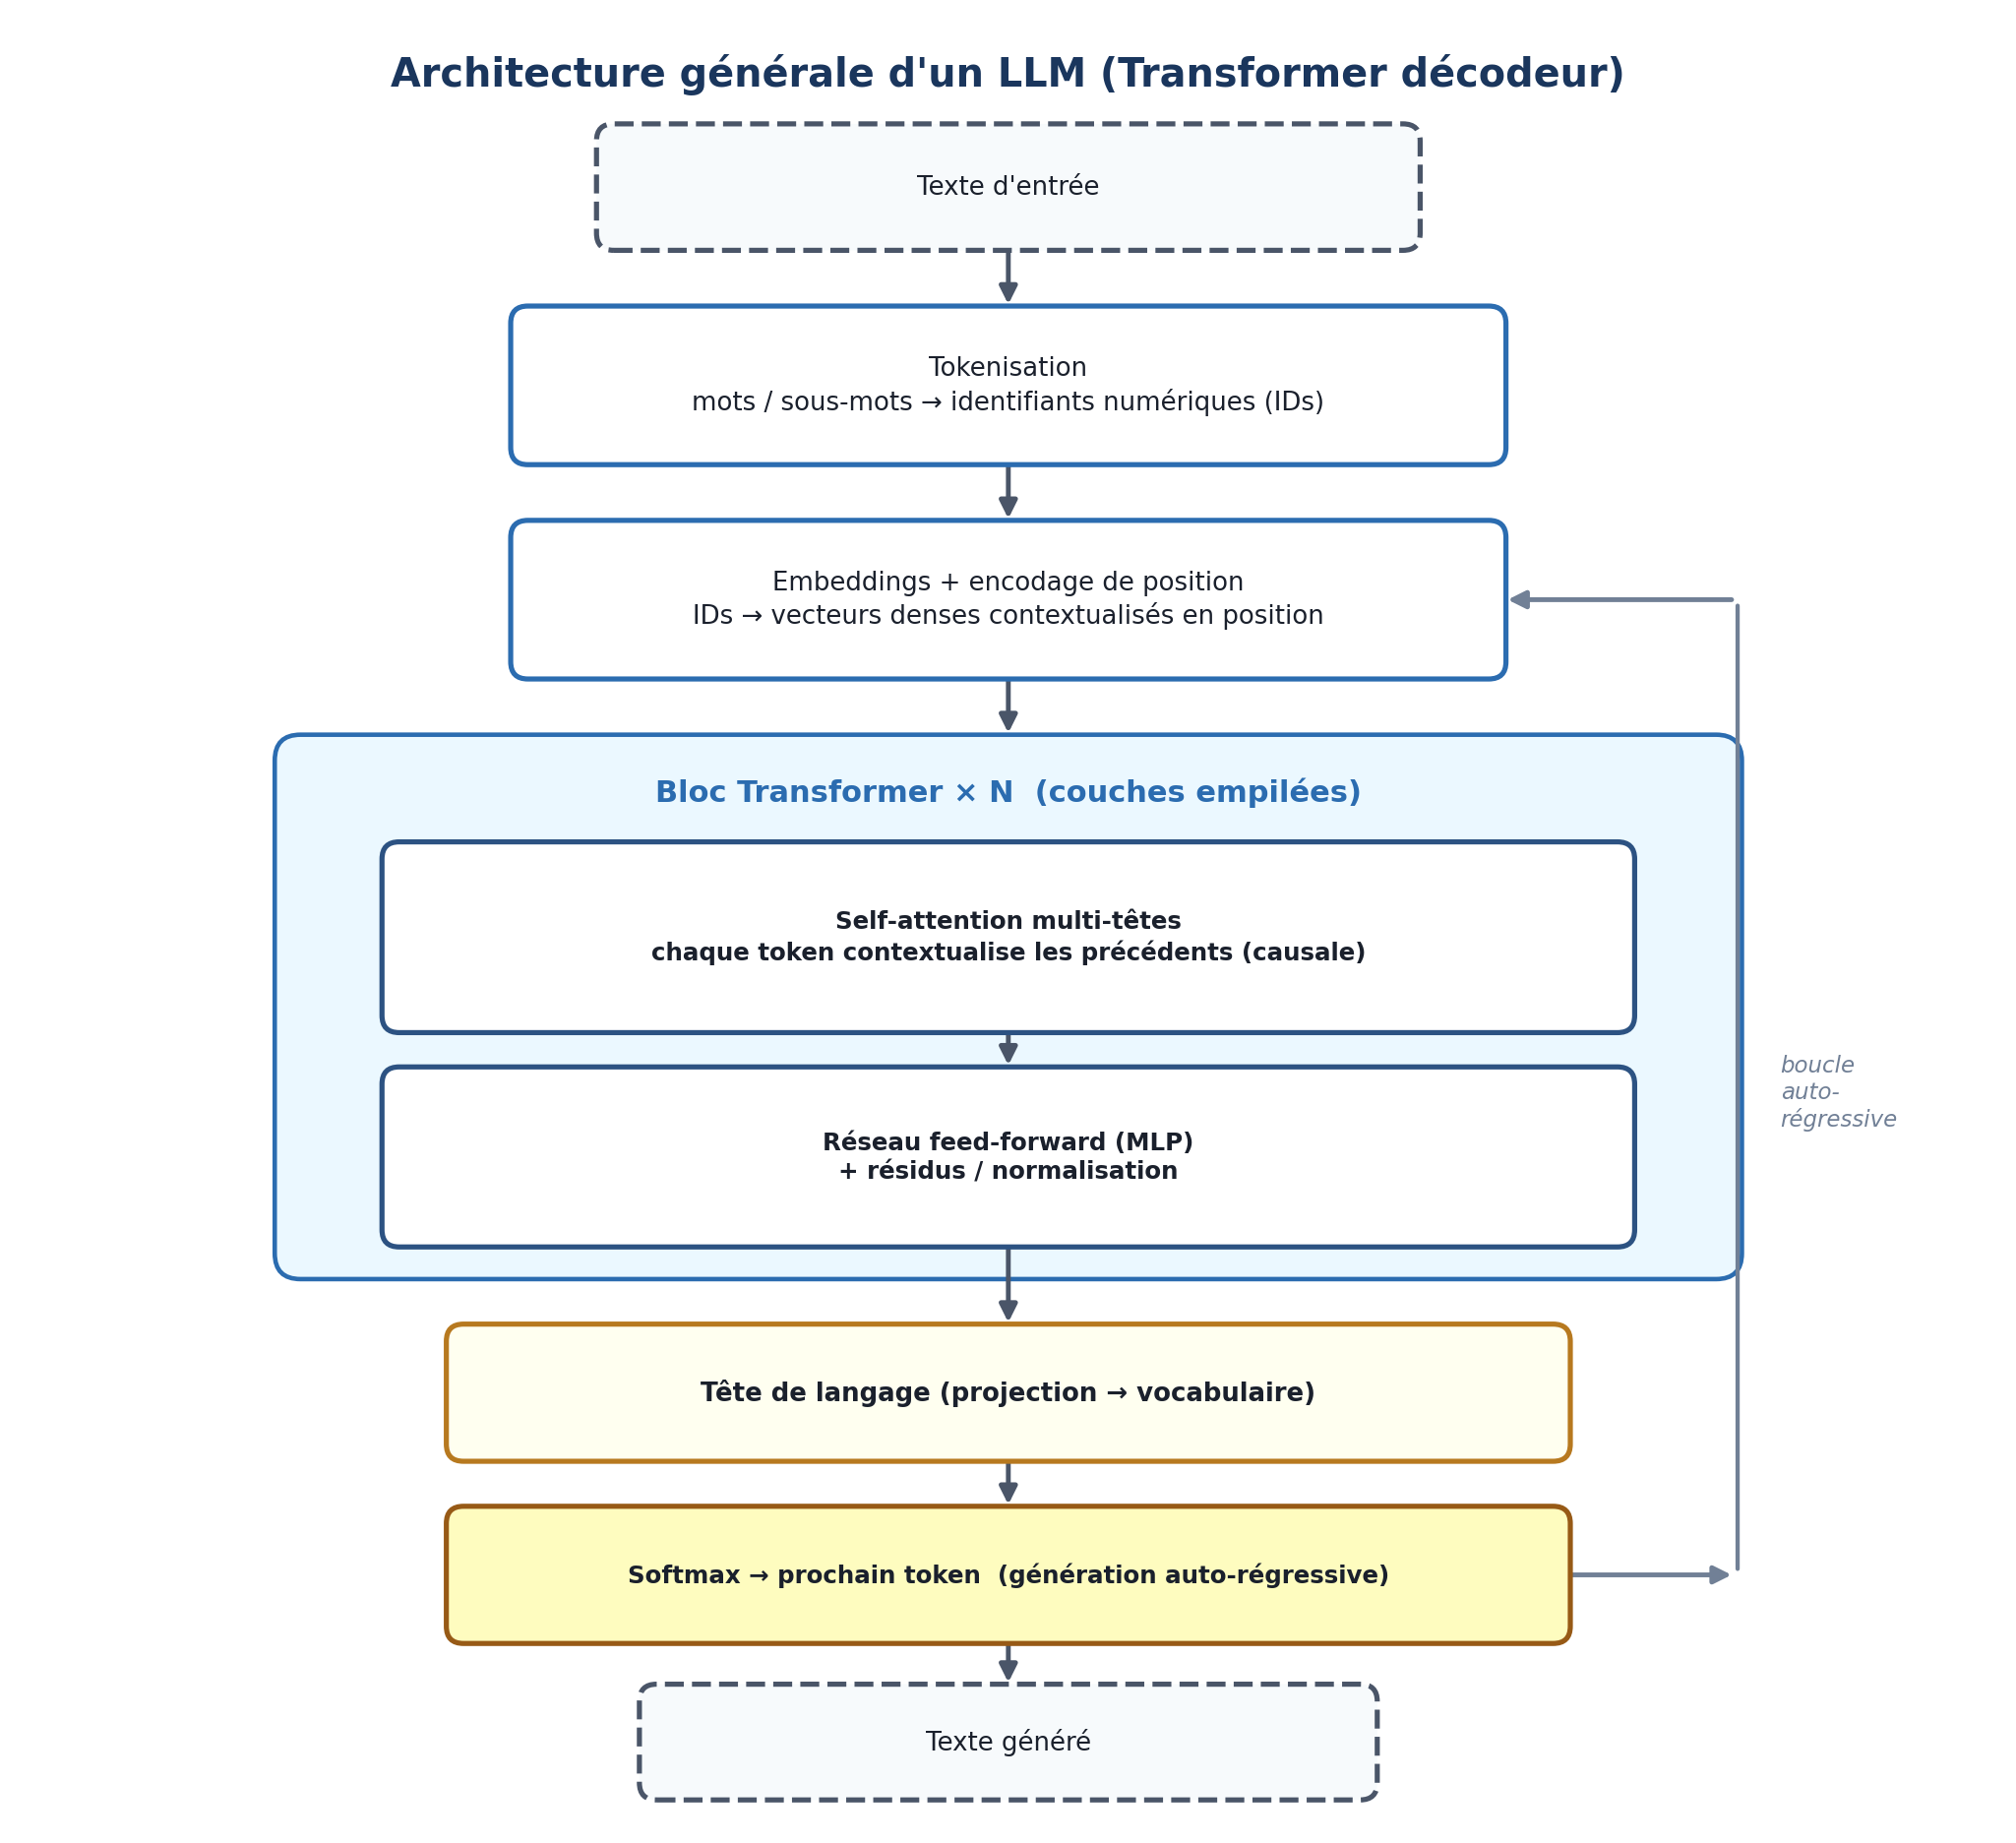
\includegraphics[width=0.88\textwidth]{figures/llm_architecture_generale.png}
\caption{Architecture générale d'un LLM de type Transformer décodeur.
}
\label{fig:fond-llm-arch}
\end{figure}

En éducation, ces modèles permettent de générer, à la demande, des
explications, reformulations, analogies ou encouragements en langage naturel
\cite{kasneci2023chatgpt,lo2023chatgpt,yan2024practical,wang2024large}. Ils offrent ainsi une voie crédible pour produire
des contenus pédagogiques personnalisés à grande échelle.

\subsection{Guidage par prompts et patrons}

La qualité du contenu généré dépend fortement du guidage
\cite{liu2023pretrain,white2023prompt,wei2022chain}. Une bibliothèque de
patrons de prompts structurés permet de conditionner la génération selon
l'état d'engagement détecté et le type d'intervention pédagogique souhaité.

\subsection{Récupération augmentée (RAG)}

Le mécanisme de \emph{Retrieval-Augmented Generation} (RAG)
\cite{lewis2020retrieval,gao2023retrieval,fan2024survey} ancre la génération sur des documents de référence
indexés dans une base vectorielle (figure~\ref{fig:fond-rag}). Les documents
sont d'abord découpés et vectorisés (indexation hors ligne). À l'exécution,
la question est embedée puis confrontée à l'index pour récupérer les
passages les plus pertinents ; ces passages enrichissent le prompt transmis
au LLM, qui produit une réponse ancrée. Ce dispositif réduit le risque
d'hallucinations factuelles et renforce la cohérence pédagogique des
contenus produits.

\begin{figure}[H]
\centering
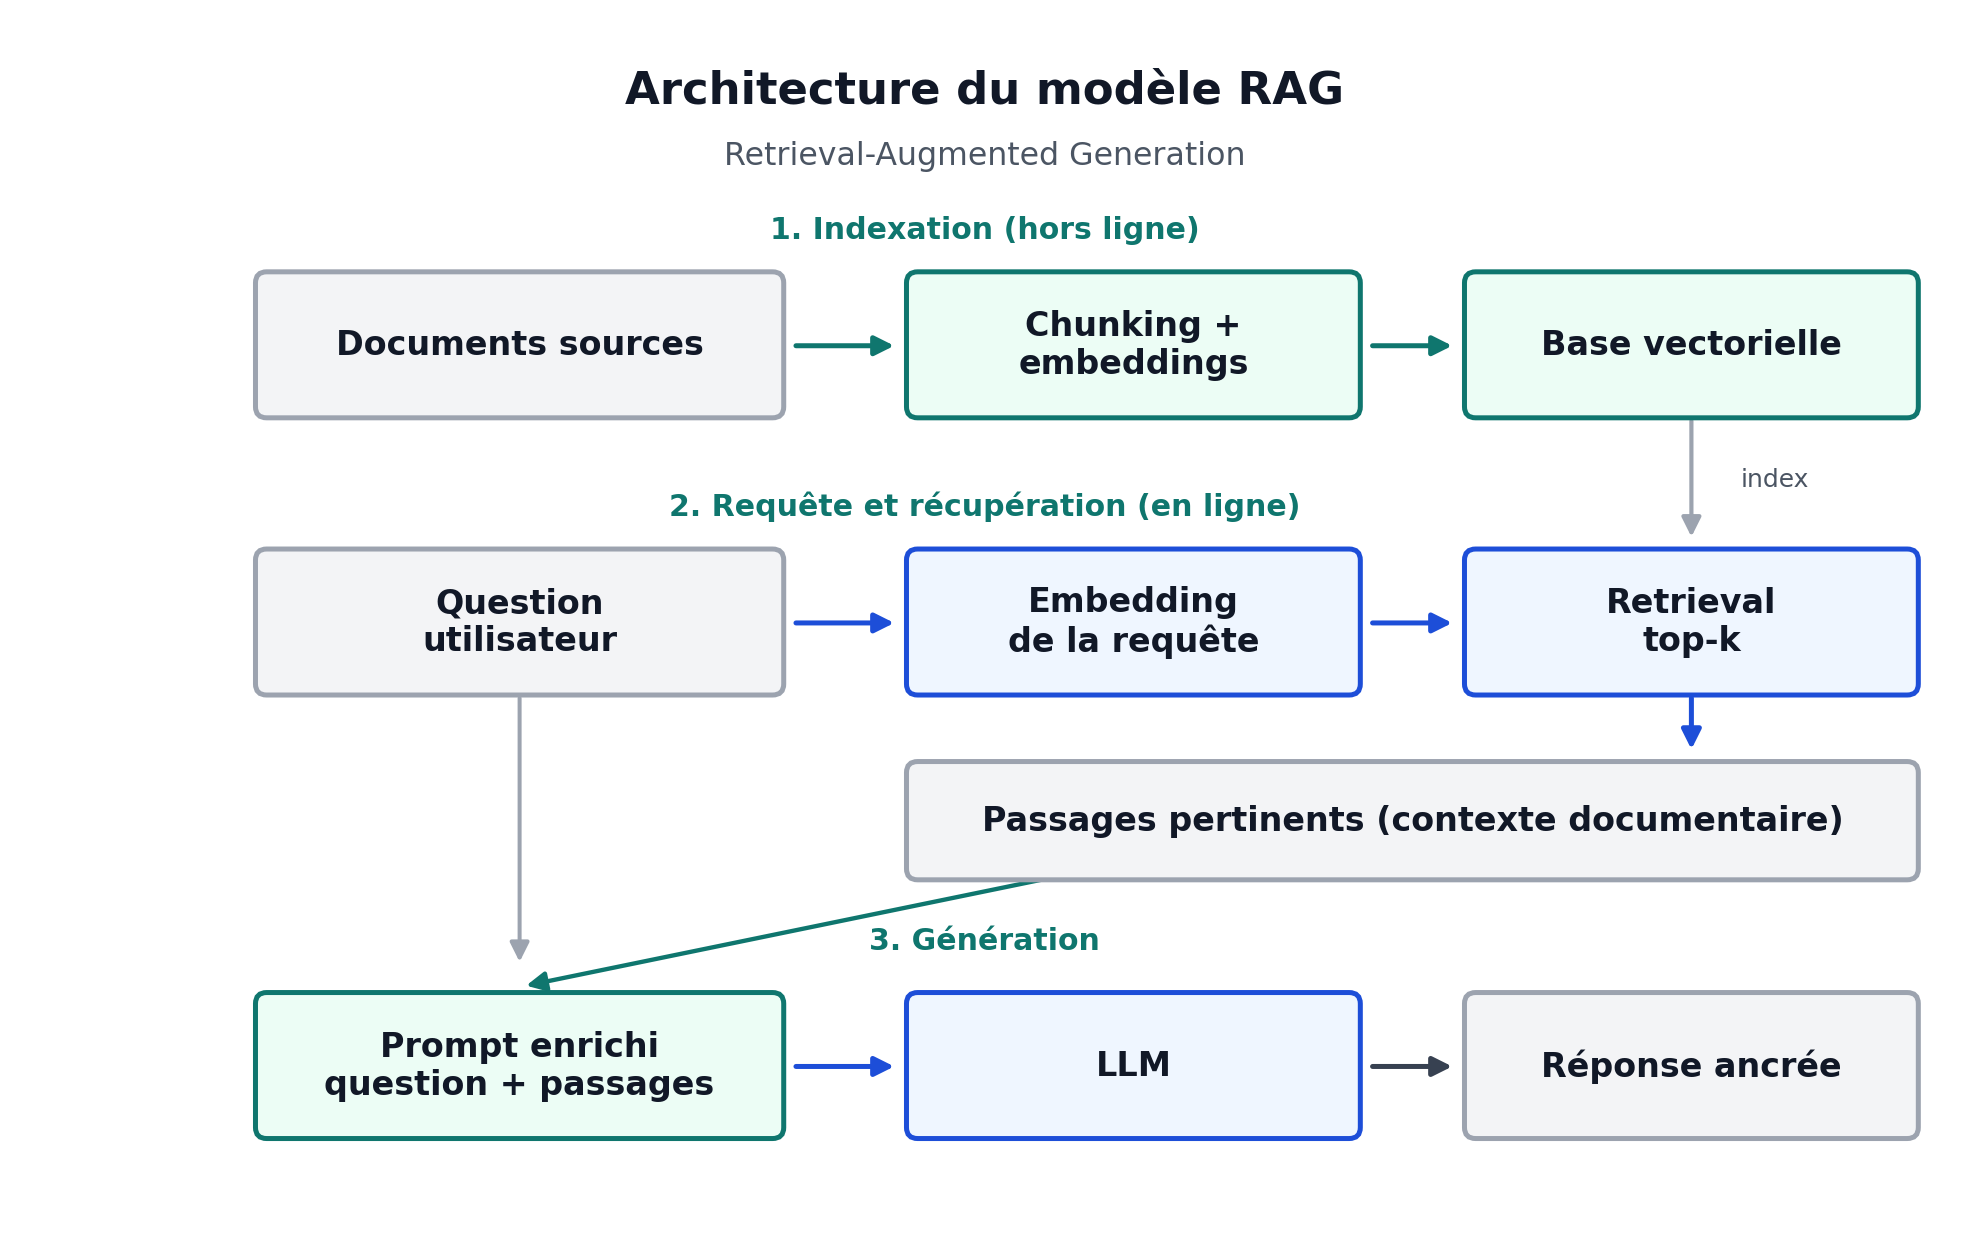
\includegraphics[width=0.92\textwidth]{figures/rag_architecture_generale.png}
\caption{Architecture générale du RAG.}
\label{fig:fond-rag}
\end{figure}

%==============================================================================
\section{Conclusion}
\label{sec:fond-concl}

Ce chapitre a rappelé le socle conceptuel sur lequel s'appuie \emolearn{} :
la définition des MOOC et l'enjeu d'adaptation, la centralité de
l'engagement émotionnel, les bases de la détection multimodale et le potentiel
de l'IA générative guidée et ancrée documentairement. Le chapitre suivant
examine l'état de l'art correspondant et positionne le présent travail par
rapport aux approches existantes.

%==============================================================================
%  CHAPITRE 2 — ÉTAT DE L'ART
%==============================================================================
\titreduchapitre{Synthèse de l'état de l'art}{chap:etat_art}

%==============================================================================
\section{Introduction}
\label{sec:ea-intro}

Le chapitre~\ref{chap:fondements} a fixé le vocabulaire. Il reste à
examiner ce que la littérature établit déjà, et ce qu'elle laisse ouvert,
lorsqu'il s'agit de réguler un apprenant isolé devant une vidéo de cours.

Deux familles de travaux se croisent sans se rejoindre pleinement. D'un
côté, on détecte l'engagement : parfois dans les messages de forum
(présence cognitive, émotions épistémiques), parfois sur le visage, la voix
ou la posture. De l'autre, on intervient : tuteurs intelligents,
règles d'adaptation, puis, depuis peu, texte généré par un grand modèle de
langue. Peu de prototypes enchaînent les deux : estimer un état, choisir une
stratégie, produire un contenu. C'est cet enchaînement que vise
\emolearn{}.

Le chapitre s'organise en six sections : MOOC et engagement apprenant,
détection automatique, psychologie des émotions, IA générative, systèmes
adaptatifs, puis synthèse critique et positionnement. Ce parcours prépare
les choix du chapitre~\ref{chap:conception}.

%==============================================================================
\section{MOOCs et engagement apprenant}
\label{sec:ea-mooc}

Trois questions structurent cette section : les défis de rétention, la
mesure de l'engagement en e-learning, puis les indicateurs émotionnels
et cognitifs.

\subsection{Défis de rétention et d'engagement}
\label{sec:ea-mooc-retention}

\textcite{daniel2012making} et \textcite{breslow2013studying}
ont d'abord décrit le MOOC comme un phénomène
d'accès ouvert à grande échelle. Les chiffres de rétention
sont connus depuis longtemps : une grande partie des inscrits part dans
les premières semaines, et le taux moyen d'achèvement stagne près de
10\,\% \cite{onah2014dropout,jordan2015massive,reich2019mooc}. Onah,
Jordan et Reich établissent ce constat. Kizilcec et Hew montrent que le
manque de temps n'explique pas à lui seul les départs : la baisse
d'engagement y contribue également
\cite{kizilcec2013deconstructing,hew2016promoting}. Le défi de rétention
porte donc aussi sur ce que les inscrits vivent pendant le cours, au-delà
du calendrier et du volume de travail déclaré.

\subsection{Mesure de l'engagement en e-learning}

L'engagement désigne la mobilisation cognitive, comportementale et
émotionnelle de l'apprenant sur une tâche \cite{fredricks2004school}. La
définition aujourd'hui la plus partagée distingue trois composantes :
\begin{itemize}
  \item l'engagement comportemental (participation, persévérance,
  effort observable)~,
  \item l'engagement cognitif (profondeur du traitement, stratégies
  d'apprentissage, présence cognitive)~,
  \item l'engagement émotionnel (intérêt, ennui, confusion,
  frustration, sentiment d'affiliation).
\end{itemize}
En e-learning, on mesure surtout des proxies : connexion, clics,
durée de session, progression, notes. Ils sont utiles, mais incomplets :
un étudiant peut rester connecté et être déjà ailleurs. Les journaux de
plateforme voient le comportement. Les forums donnent un aperçu de la
cognition, à condition que l'étudiant écrive. Compter les clics ne
suffit donc plus : il faut une mesure plus proche de ce que l'apprenant
est en train de vivre
\cite{kizilcec2013deconstructing,dmello2015review}.

\subsection{Indicateurs émotionnels et cognitifs}

L'émotion, pourtant liée à la persévérance
\cite{pekrun2006control,dmello2012dynamics}, n'apparaît pas dans les logs.
\emolearn{} s'appuie sur ces indicateurs, dans l'hypothèse qu'une
régulation plus précoce agit sur la suite du parcours. L'étude de Liu \emph{et al.} sur le forum d'\emph{Introduction
to Psychology} (8\,867 inscrits) va dans ce sens : émotion et cognition
bougent ensemble, et prédisent mieux la réussite lorsqu'on les lit
conjointement \cite{liu2022automated}. Un seul score d'\og engagement \fg{}
efface ces nuances.

Dès que l'on dispose de texte, la revue de Sakeef \emph{et al.} montre que
trois grilles reviennent pour coder l'engagement cognitif des
forums \cite{sakeef2025detecting}. La plus citée est le modèle de
Community of Inquiry \cite{garrison1999critical} : présence sociale,
enseignante et cognitive, cette dernière en quatre phases (déclenchement,
exploration, intégration, résolution). Hu \emph{et al.} et Liu \emph{et al.}
s'en servent pour entraîner des classifieurs
\cite{hu2021automatic,liu2023moocbert}. ICAP, proposé par Chi et Wylie,
classe plutôt le mode d'activité : passif, actif, constructif,
interactif \cite{chi2014icap}. Plus on construit ou on interagit, plus le
traitement est censé être profond.

Ces indicateurs cognitifs aident à relire un fil de discussion
après coup. Ils disent peu d'un visionnage sans contribution
écrite. Dans ce cas, les indicateurs émotionnels visibles, taxonomie
\textsc{DAiSEE} : engagement, ennui, confusion, frustration sont plus
directs : un état, un besoin pédagogique \cite{gupta2016daisee}.

%==============================================================================
\section{Détection automatique de l'engagement}
\label{sec:ea-detection}

On ne peut pas demander à un enseignant de coder des milliers de messages,
ni d'observer chaque visage. D'où l'intérêt d'un estimateur automatique.
Cette section examine trois axes : les approches multimodales (visuelle,
comportementale, physiologique), les corpus publics (\textsc{DAiSEE},
\textsc{EmotiW}, et les ressources complémentaires), puis les performances
rapportées dans la littérature. Les scores d'\emolearn{} lui-même (FER+AU,
WavLM, fusion) sont ceux du chapitre~\ref{chap:validation}, ils ne
constituent pas un palmarès de l'état de l'art.

\subsection{Approches multimodales}
\label{sec:ea-detection-multimodal}

D'Mello, dans sa méta-analyse, insiste sur un point pratique : ennui,
confusion, frustration et engagement reviennent souvent, et mélanger les
modalités aide, à condition de calibrer \cite{dmello2015review}. Trois
familles de signaux structurent cet axe.

\paragraph{Voie visuelle:}
En l'absence de production écrite, le signal disponible est celui que
l'on peut filmer. Whitehill \emph{et al.} ont montré, dès 2014, qu'un
classifieur de visage
peut approcher le jugement humain sur l'engagement
\cite{whitehill2014faces}. Depuis, les réseaux profonds et les Transformers
ont relevé le niveau \cite{li2020deepfer,dosovitskiy2021vit}. En classe,
d'autres travaux suivent le regard ou le décrochage attentionnel
\cite{goldberg2021attentive,hutt2021automated}. Sur \textsc{DAiSEE},
plusieurs architectures hybrides spatio-temporelles ont été testées
\cite{abedi2021improving,gupta2023multimodal}.

Xiong, Guo et Xu proposent un CNN-Transformer qui combine l'information
fine des expressions faciales (CNN) et l'information plus grossière de la
posture (Transformer), en réduisant l'encombrement visuel du fond
\cite{xiong2024cnntransformer}. Sur un jeu de données de classe réelle,
annoté par crowdsourcing puis validation experte, le modèle atteint
92,9\,\% d'accuracy et surpasse plusieurs architectures de deep learning.
Ce travail est le plus proche d'\emolearn{} du point de vue du
signal (vision en situation d'apprentissage). Il s'en distingue
toutefois sur deux points décisifs : il ne fusionne pas la voix, et il ne
relie pas la détection à une génération de contenu. L'identification
s'arrête au diagnostic.

Côté voix: souvent traitée à part, mais bien une modalité perceptive,
le passage des descripteurs acoustiques classiques aux représentations
auto-supervisées (WavLM), évaluées notamment via le
benchmark SUPERB, a transformé la reconnaissance
d'émotions vocales
\cite{chen2022wavlm,pepino2021emotion,yang2021superb,latif2023survey}.
Le fine-tuning de ces encodeurs \cite{chen2023exploring} et les
architectures Transformer réduisent notamment l'écart de performance
sur la valence, longtemps le point faible du SER
\cite{wagner2023dawn}. Ces avancées justifient le choix actuel
d'\emolearn{} : un encodeur WavLM fine-tuné vers les quatre
états \textsc{DAiSEE}, complété par une ancre émotionnelle
\textsc{IEMOCAP}, plutôt que des seuils acoustiques ou un simple mapping
émotion\,$\rightarrow$\,engagement. Côté visage, le runtime retient un
Random Forest FER+AU (sept scores d'un ViT pré-entraîné, plus
Action Units) comme juge produit, un ViT fine-tuné vers les quatre
états filtre les images peu confiantes et sert de mode dégradé, sans
choisir l'état transmis à la fusion.

\paragraph{Voie comportementale:}
On rassemble ici les traces d'activité: clics, durée de session,
progression dans un MOOC, souris, posture, et le texte laissé sur un forum.
Kizilcec et al. montrent que ces proxies séparent des
sous-populations d'inscrits, sans dire ce que l'étudiant est en train de
vivre \cite{kizilcec2013deconstructing}. La posture, chez Xiong, est déjà
un signal comportemental filmé \cite{xiong2024cnntransformer}. Dans les
MOOC, le matériau comportemental le plus riche reste le texte des
forums.

Sakeef \emph{et al.} proposent une revue des cadres (CoI, ICAP, KCSA) et des
méthodes de TALN / apprentissage profond utilisées pour détecter l'engagement
cognitif dans ces messages \cite{sakeef2025detecting}. Ils soulignent que
l'annotation manuelle est trop coûteuse pour un suivi en continu, et que
l'automatisation devient indispensable. Ils rappellent aussi une limite
structurelle : l'absence d'indices visuels et auditifs dans le texte rend
l'inférence de l'état interne partielle. Cette limite motive, pour
\emolearn{}, le recours aux modalités visage et voix (corpus annotés)
plutôt qu'au seul forum.

Hu, Ferreira Mello et Gašević comparent un CNN à des Random Forests
fondés sur des traits linguistiques pour classer la présence cognitive
selon le CoI \cite{hu2021automatic}. Le CNN atteint un $\kappa$ de Cohen de
0,528, comparable aux approches classiques, avec une généralisabilité
inter-cours similaire. L'apport principal est l'explicabilité (XAI) au
niveau des mots. Le travail reste une tâche de catégorisation de messages,
sans lien avec une intervention pédagogique automatique.

Liu \emph{et al.} (2022) introduisent BERT-CNN pour détecter conjointement
l'engagement émotionnel et cognitif dans le forum du MOOC
\emph{Introduction to Psychology}
\cite{liu2022automated}. Par rapport aux modèles antérieurs, le F1
s'améliore d'environ 10\,\% (émotion) et 8\,\% (cognition).
Méthodologiquement, le papier établit qu'un détecteur robuste est un
prérequis à toute régulation, opérationnellement, il s'arrête à la
prédiction de la réussite, sans générer de contenu adaptatif.

MOOC-BERT pousse plus loin le pré-entraînement : le modèle est pré-entraîné
sur le MOOC-Corpus (icourse163.org : 800 cours, cinq disciplines,
3{,}76~Go), puis fine-tuné pour identifier la présence cognitive
\cite{liu2023moocbert}. Il surpasse les algorithmes représentatifs, y
compris en généralisation inter-cours. La boucle s'arrête à l'aide à
l'enseignant : fournir un diagnostic, non produire l'intervention.

Liu \emph{et al.} (2021) articulent analyse de réseaux sociaux et analyse de
réseaux épistémiques sur 3\,925 participants d'un forum MOOC
\cite{liu2021exploring}. Les groupes à haute et basse réussite diffèrent
en centralité, les connexions cognitives sont plus fortes chez les
apprenants performants. Ce résultat concerne une dynamique
collective (forum), distincte du scénario individuel visé par
\emolearn{}.

\paragraph{Voie physiologique:}
Une troisième famille EEG, réponse électrodermale, rythme cardiaque,
parfois ECG existe surtout en laboratoire
\cite{picard1997affective,dmello2015review,abedi2021improving}. Elle sort du
périmètre d'\emolearn{} : le scénario visé est une vidéo de cours, avec
webcam et microphone, sans capteur médical.

\subsection{Datasets publics d'engagement}
\label{sec:ea-detection-datasets}

Les corpus visuels publics d'engagement restent rares. On en
retient ici ce qui structure la détection.

\textsc{DAiSEE} fournit des vidéos d'apprenants annotées en quatre états
(engagement, ennui, confusion, frustration), chacun sur une intensité de
0 à 3, en conditions naturelles (\og dans la nature \fg{})
\cite{gupta2016daisee}. La classe Engagement y domine largement, ce qui
rend l'exactitude globale insuffisante comme seule métrique. C'est la taxonomie retenue par
\emolearn{}, parce que chaque état appelle une réponse pédagogique
distincte.

Le défi \textsc{EmotiW} propose aussi des pistes \og dans la nature \fg{}, dont une
tâche d'engagement étudiant \cite{dhall2018emotiw}. Les étiquettes y sont
surtout des niveaux d'engagement, pas les quatre états
pédagogiques de \textsc{DAiSEE}. Les scores des éditions successives ne se
lisent donc pas comme un classement sur le même problème.

\textsc{IEMOCAP} offre un signal vocal riche et, dans sa version
audiovisuelle, un cadre où visage et voix proviennent du même locuteur
\cite{busso2008iemocap}. Les étiquettes y décrivent l'émotion dyadique,
et non l'engagement d'un apprenant en MOOC. \emolearn{} s'appuie
explicitement sur ces deux ressources complémentaires : \textsc{DAiSEE}
pour la taxonomie d'engagement facial, \textsc{IEMOCAP} pour l'émotion
vocale.

D'autres jeux restent propriétaires : Whitehill \emph{et al.}
annotent leurs propres vidéos d'étudiants \cite{whitehill2014faces}, 
Xiong \emph{et al.} collectent des images de classe faute de dataset
ouvert alliant visage et posture \cite{xiong2024cnntransformer}. Les
travaux sur forums (icourse163.org, bancs CoI) et les essais PAGE ou Kong
n'offrent pas un dataset public d'engagement visuel.

\subsection{État de l'art des performances de détection}
\label{sec:ea-detection-perfs}

Comparer un $\kappa$ sur du texte CoI, une accuracy sur quatre niveaux  \textsc{DAiSEE} et 92,9\,\% sur un corpus de classe privé
n'a de sens que si l'on rappelle que la tâche n'est pas la même.
Le tableau~\ref{tab:ea-perfs-detection} présente les chiffres
effectivement rapportés par les articles déjà discutés. Il ne prétend pas
couronner un vainqueur unique.

{\scriptsize
\setlength{\tabcolsep}{3pt}
\renewcommand{\arraystretch}{1.08}
\begin{xltabular}{\textwidth}{|>{\raggedright\arraybackslash}X|>{\raggedright\arraybackslash}X|>{\raggedright\arraybackslash}X|>{\raggedright\arraybackslash}X|}
\hline
\rowcolor{gray!20}
\textbf{Référence} & \textbf{Tâche / signal} & \textbf{Corpus} &
Résultat clé \\
\hline
\endfirsthead
\hline
\rowcolor{gray!20}
\textbf{Référence} & \textbf{Tâche / signal} & \textbf{Corpus} &
Résultat clé \\
\hline
\endhead
\endfoot
\endlastfoot
\textcite{whitehill2014faces}
  & Visage, 4 niveaux d'engagement
  & Corpus propre (non public)
  & Accord proche des annotateurs humains, \textcite{gupta2016daisee} rappellent $\approx 69\,\%$ pour SVM + Gabor \\
\hline
\textcite{gupta2016daisee}
  & Vidéo, 4 niveaux d'engagement
  & \textsc{DAiSEE} (public)
  & Baselines des auteurs : InceptionNet $46{,}4\,\%$, C3D $56{,}1\,\%$, LRCN $57{,}9\,\%$ \\
\hline
\textcite{abedi2021improving}
  & Vidéo spatio-temporelle, 4 niveaux
  & \textsc{DAiSEE}
  & ResNet+TCN : $63{,}9\,\%$ d'accuracy (mieux que les baselines \textsc{DAiSEE} et plusieurs hybrides) \\
\hline
\textcite{xiong2024cnntransformer}
  & Visage + posture, 4 niveaux
  & Images de classe (propre)
  & Accuracy $92{,}9\,\%$, pas de voix, corpus non public \\
\hline
\textcite{hu2021automatic}
  & Texte, phases CoI
  & Deux cours annotés
  & $\kappa$ de Cohen $= 0{,}528$ (CNN $\approx$ Random Forests) \\
\hline
\textcite{liu2022automated}
  & Forum, émotion + cognition
  & icourse163.org ($n=8\,867$)
  & F1 $+10\,\%$ (émotion) et $+8\,\%$ (cognition) vs modèles antérieurs \\
\hline
\textsc{EmotiW} \cite{dhall2018emotiw}
  & Engagement \og dans la nature \fg{}
  & Pistes du défi (public)
  & Scores d'édition en édition, niveaux d'engagement, non comparables à la taxonomie \textsc{DAiSEE} \\
\hline
\end{xltabular}
\xlcaption{Performances de détection rapportées.}
\label{tab:ea-perfs-detection}
}

Deux lectures s'imposent. Premièrement, sur \textsc{DAiSEE}, même les
meilleures architectures citées ici restent dans une fourchette d'accuracy
modérée ($57{,}9\,\%$ à $63{,}9\,\%$ pour quatre niveaux d'engagement),
parce que la classe haute domine : un classifieur naïf « toujours
engagé » paraît déjà fort. C'est pourquoi \emolearn{} retient, au
chapitre~\ref{chap:validation}, le F1 macro et le rappel des états
urgents plutôt que l'accuracy seule. Deuxièmement, un score élevé sur un
corpus privé (Xiong) ou un $\kappa$ sur du CoI ne se substitue pas à une
évaluation visage--voix vers les quatre états \textsc{DAiSEE}.

Identifier un état ne suffit pas à justifier son importance pédagogique,
ni à en déduire une intervention. La section suivante rappelle les
fondements psychologiques, les deux suivantes traitent de la génération
et des systèmes adaptatifs.

%==============================================================================
\section{Psychologie de l'apprentissage et émotions}
\label{sec:ea-psycho}

Les cadres sur les MOOC et l'engagement indiquent quoi mesurer.
Ils disent moins \emph{pourquoi} un état change la suite du parcours. Trois
points sont examinés : l'impact des émotions, les théories de la charge
cognitive, puis les états d'engagement (ennui, confusion,
frustration, flow).

\subsection{Impact des émotions sur l'apprentissage}

Picard et Pekrun ont, chacun de leur côté, rappelé que l'émotion n'est pas
un bruit autour de la cognition : elle oriente l'attention et la
persévérance \cite{picard1997affective,pekrun2006control}. Les revues
récentes sur les environnements technologiques aboutissent au même constat
\cite{loderer2020beyond,graesser2020emotions}. Une émotion n'est donc pas
un à-côté du cours : elle décide, en partie, si l'étudiant reste ou part.

\subsection{Théories de la charge cognitive}

Sweller décrit le couple sous l'angle de la charge : trop de matière à la
fois, et l'étudiant se perd (surcharge, confusion), trop peu, et il
décroche (sous-stimulation, ennui)
\cite{sweller1988cognitive,sweller2019cognitive}. Les développements
ultérieurs distinguent charge intrinsèque (difficulté de la matière),
charge extrinsèque (présentation maladroite) et charge germane (effort
utile). Mayer, pour le multimédia, montre que le rythme, le texte et
l'image pèsent sur cette charge utile \cite{mayer2021multimedia}. Un
parcours unique, calé sur un « étudiant moyen », rate ces bascules :
c'est précisément ce qu'une adaptation par état cherche à éviter.

\subsection{États d'engagement : ennui, confusion, frustration, flow}

Quatre états, issus de \textsc{DAiSEE}, structurent la suite du mémoire
\cite{gupta2016daisee} :
\begin{itemize}
  \item L'engagement : implication positive, traitement en cours.
    on maintient ou on enrichit.
  \item L'ennui : sous-stimulation, amorce de
    retrait, on relance.
  \item La confusion : incompréhension encore active, on clarifie.
  \item La frustration : blocage, on soutient et on simplifie.
\end{itemize}
Chacun est annoté sur une intensité de 0 à 3. Distinguer ces états n'est
pas un luxe de taxonomie : chacun appelle une réponse différente.

Le flow de Csikszentmihalyi désigne le pôle productif : un
engagement soutenu quand le défi et les compétences s'équilibrent
\cite{csikszentmihalyi1990flow}. \textsc{DAiSEE} ne l'annote pas à part, 
l'état Engagement en est le proxy opératoire. On retient donc le flow
comme cadre théorique, et les quatre labels \textsc{DAiSEE} comme
taxonomie de détection.

D'Mello et Graesser suivent une séquence souvent observée en EIAH
(environnements informatiques pour l'apprentissage humain) : la
confusion, si elle se résout, aide (et peut ramener vers le flow), si elle
s'enlise, elle glisse vers la frustration, puis vers l'ennui
\cite{dmello2012dynamics}. Baker \emph{et al.} en concluent que
la frustration reste préférable à l'ennui, car la première suppose
un effort, le second un retrait \cite{baker2010better}. Cette réserve de
contexte compte : l'observation a été formulée dans des tuteurs
intelligents, plutôt que lors d'un visionnage isolé de cours en ligne.
Elle indique qu'un désengagement sans expression est, pédagogiquement,
plus grave qu'un blocage encore actif.

%==============================================================================
\section{IA générative pour l'éducation}
\label{sec:ea-genai}

Les tuteurs intelligents adaptent souvent un
contenu déjà écrit. Les grands modèles de langue rendent possible de le produire à la demande. Quatre axes sont examinés : génération
pédagogique, ingénierie de prompts, personnalisation, puis évaluation de
la qualité.

\subsection{LLMs et génération de contenu pédagogique}

Depuis GPT-3 et les modèles de la famille Llama, un grand modèle de langue
peut rédiger une explication, une analogie, un exercice ou un encouragement
en quelques secondes
\cite{brown2020language,touvron2023llama}. \textcite{kasneci2023chatgpt} ont très tôt
listé ce que cela change pour l'école : personnalisation possible, mais aussi
erreurs factuelles, biais, et décisions difficiles à retracer. Les revues qui ont suivi (Lo, Yan, Bond, entre
autres) ne contredisent pas ce constat
\cite{lo2023chatgpt,yan2024practical,bond2024systematic}. Laissé libre, le
modèle écrit « comme un cours » sans garantir que le cours soit juste.

Un garde-fou fréquent, distinct du prompt, est le RAG : on récupère d'abord
des extraits d'une base documentaire, puis on les fournit au modèle
\cite{lewis2020retrieval}. C'est ce mécanisme qu'\emolearn{} retient pour
coller le texte généré à des fiches de cours, plutôt que de le laisser
inventer une définition. Le LLM n'est donc pas, ici, un enseignant
autonome : c'est un rédacteur conditionné par une décision déjà prise
et par des documents vérifiés.

\subsection{Prompt engineering pour applications éducatives}

La qualité du texte dépend fortement du guidage : rôle, format, longueur,
exemples \cite{liu2023pretrain,white2023prompt,wei2022chain}. En éducation,
un prompt trop vague produit un cours générique, un prompt trop serré
peut brider l'utilité. Les patrons structurés permettent de conditionner
la génération selon l'état visé et le type d'intervention (clarifier,
exemplifier, exercer, soutenir).

Liu \emph{et al.} (2025) poussent le prompt dans une autre direction : non
pour écrire un cours, mais pour étiqueter un message (comportement,
émotion, cognition) \cite{liu2025agka}. Leur méthode AGKA ajoute au prompt
les définitions du guide d'annotation et quelques exemples. GPT-4 et
Llama~3 70B s'en sortent alors aussi bien que BERT sur des tâches binaires, 
dès que les classes se ressemblent (émotions épistémiques, phases CoI),
l'écart se creuse. On en retient surtout ceci : un LLM guidé peut aider à
classer du texte, il ne remplace pas un détecteur visage--voix.
\emolearn{} fait l'inverse : le modèle n'étiquette pas l'état, il rédige
le contenu après que la couche de perception a décidé, via une
bibliothèque de vingt patrons.

\subsection{Personnalisation et adaptation automatique}

Hu et Shao proposent PAGE (\emph{Psychologically-Aware Generative Education}),
un système GenAI qui adapte le style, la difficulté et les mécanismes de
soutien au profil Big Five et au feedback émotionnel en temps réel
\cite{hu2025page}. Sur 200 étudiants, PAGE améliore la satisfaction
émotionnelle (4,4/5 contre 3,6/5), le taux de complétion des tâches
(87,6\,\% contre 72,3\,\%) et la durée d'étude (+34\,\%) par rapport à un
système adaptatif classique, le bénéfice est particulièrement marqué pour
les étudiants à neuroticisme élevé (baisse de 48\,\% du décrochage). PAGE
est le travail le plus proche d'\emolearn{} du point de vue de la génération : il relie un signal affectif à un contenu produit par
LLM. L'écart se joue sur le quand et le comment. PAGE s'appuie sur
un profil Big Five (assez stable) et sur un retour émotionnel souvent
déclaré. Le présent travail vise l'état de ce clip : confusion
maintenant, ennui après trois minutes. PAGE ne décrit pas non plus un
moteur de règles nommé, ni un RAG sur fiches de cours : le style change,
mais on ne peut pas retracer « tel état $\rightarrow$ tel patron ».

Kong \emph{et al.} évaluent un autre mode d'adaptation : un outil de
représentation des discussions assisté par IA (représentations
comportementales, cognitives, ou mixtes) auprès de 122 étudiants
\cite{kong2025exploratory}. L'outil n'améliore pas significativement la
motivation, mais augmente la présence cognitive de haut niveau et la
performance. Il s'agit d'une médiation sur le forum, non d'une
génération de contenu de cours conditionnée par l'état d'un apprenant
isolé. Le résultat confirme qu'une personnalisation IA peut élever le
niveau cognitif, à condition d'en changer le canal (vidéo de cours plutôt
que fil de discussion).

\subsection{Évaluation de la qualité pédagogique}

La qualité du contenu généré se juge sur des critères humains (pertinence,
clarté, adéquation à l'état) complétés par des métriques automatiques de
forme (longueur, lisibilité, respect du patron). Aucune métrique automatique
ne se substitue à une validation experte ou utilisateur
\cite{kasneci2023chatgpt,hu2025page}. Les travaux de détection rapportent
surtout des F1 et des $\kappa$, les travaux génératifs rapportent des scores
de satisfaction. Un protocole multi-niveaux (perception, décision,
génération) reste rare. C'est l'un des choix méthodologiques d'\emolearn{}.

%==============================================================================
\section{Systèmes adaptatifs d'apprentissage}
\label{sec:ea-its}

Identifier un état ne suffit pas à en déduire une intervention. Les
tuteurs intelligents en sont le précédent le plus net : un modèle de
l'apprenant, une stratégie, un contenu. Trois étages sont distingués ici :
ce que sont les ITS, quelles stratégies pédagogiques ils mobilisent, puis
comment la décision est formalisée (règles et modèles).

\subsection{Intelligent Tutoring Systems (ITS)}

Les systèmes de tutorat intelligent (ITS) combinent historiquement un modèle
de l'apprenant, un modèle pédagogique et une interface adaptative
\cite{vanlehn2011relative}. VanLehn montre que les meilleurs ITS approchent
l'efficacité d'un tuteur humain, à condition que le domaine soit bien
modélisé \cite{vanlehn2011relative}. Le contenu est le plus souvent
pré-écrit : chaque rétroaction a été rédigée à l'avance pour un état
de connaissances prévu.

Deux familles d'exemples illustrent ce schéma sans en changer la
logique. Les tuteurs cognitifs, dont la revue de VanLehn rend compte,
adaptent surtout la prochaine étape d'un parcours : l'item suivant,
un indice, une remédiation calée sur ce que l'apprenant maîtrise encore
mal. Les tuteurs affectifs, dont AutoTutor et les dynamiques décrites par
D'Mello et Graesser sont les références les plus citées, observent aussi
la confusion ou la frustration pendant le dialogue, puis ajustent
l'étayage \cite{dmello2012dynamics,graesser2020emotions}. Dans les deux cas,
l'intervention reste choisie dans un répertoire d'auteurs, pas rédigée à
la demande.

Leur limite, dans un MOOC aux contenus ouverts et aux états affectifs
fluctuants, est double. D'une part, on ne peut pas pré-écrire un texte pour
chaque combinaison d'état et de concept. D'autre part, le modèle de
l'apprenant est surtout cognitif (ce qu'il sait), rarement émotionnel (s'il
s'ennuie ou s'il est bloqué), même si des travaux récents visent une
explication personnalisée des décisions de tuteurs \cite{conati2021toward}.
C'est cette limite que les modèles de langue visent à lever : générer le
contenu, tout en gardant une décision lisible.

\subsection{Stratégies d'adaptation pédagogique}

Les stratégies d'adaptation classiques ne portent pas sur quel
algorithme détecte l'état, mais sur l'action à entreprendre une fois
l'état connu. On distingue notamment la simplification (réduire
la charge, Sweller), l'enrichissement (approfondir lorsque
l'apprenant est déjà engagé), la remédiation (revenir sur un
point mal compris) et l'encouragement (soutenir un effort qui
s'enlise) \cite{sweller1988cognitive,vanlehn2011relative}.

Ces familles se recoupent avec les quatre états \textsc{DAiSEE} : la
confusion appelle plutôt une clarification, la frustration un soutien et
une simplification, l'ennui une relance, l'engagement un maintien ou un
enrichissement. PAGE adapte plutôt le style et la
difficulté à un profil de personnalité \cite{hu2025page}, les ITS
adaptent surtout la prochaine étape d'un parcours cognitif. Dans
les deux cas, une stratégie sans contenu à produire (ou sans règle pour
la choisir) reste un principe, pas un système.

\subsection{Règles et modèles de décision}

Deux grandes manières de décider coexistent. Les modèles
cognitifs (traçage bayésien des connaissances, théorie des espaces de
connaissances) estiment ce que l'apprenant maîtrise, puis sélectionnent
un item \cite{vanlehn2011relative}. Les règles explicites
relient un état observé à une action nommée, au prix d'une rigidité, mais
avec une traçabilité que Conati \emph{et al.} jugent utile pour expliquer
un tuteur \cite{conati2021toward}.

\emolearn{} se place délibérément du côté des règles. Une matrice
\emph{état\,$\rightarrow$\,type de contenu} (explication, exemple,
exercice, encouragement) fixe le quoi, des règles temporelles sur
les séquences de clips fixent le quand (un épisode isolé n'a pas le
même poids qu'une frustration qui dure). Le moteur reste interprétable :
chaque adaptation doit être justifiable par l'état détecté, la stratégie
retenue et le patron mobilisé. Le détail de cette matrice appartient au
chapitre~\ref{chap:conception}, l'état de l'art retient surtout le
principe : sans règle nommée, la génération n'est plus une décision
pédagogique, c'est une improvisation.

%==============================================================================
\section{Synthèse critique et positionnement}
\label{sec:ea-synthese}

Cette section clôt l'état de l'art par une lecture critique des
travaux (ce qu'ils établissent, ce qu'ils laissent ouvert), puis par le
positionnement d'\emolearn{}. Le tableau~\ref{tab:ea-comparatif} en
est l'instrument : référence, approche / modèle, contexte, forces, limites,
résultats clés. Ce tableau compare des méthodes. Il se lit
par blocs (cadres et corpus, puis détection, ITS et génération), plutôt
que comme un classement unique.

\providecommand{\eatabhead}{}
\renewcommand{\eatabhead}{%
\rowcolor{gray!20}
\textbf{Référence} & \textbf{Approche / modèle} & \textbf{Contexte} &
\textbf{Forces} & Limites & Résultats clés \\}

Le tableau~\ref{tab:ea-comparatif} présente la synthèse critique des travaux retenus.

{\scriptsize
\setlength{\tabcolsep}{2.4pt}
\setlength{\LTcapwidth}{\textwidth}
\renewcommand{\arraystretch}{1.08}
\begin{xltabular}{\textwidth}{|>{\raggedright\arraybackslash}X|>{\raggedright\arraybackslash}X|>{\raggedright\arraybackslash}X|>{\raggedright\arraybackslash}X|>{\raggedright\arraybackslash}X|>{\raggedright\arraybackslash}X|}
\hline
\eatabhead
\hline
\endfirsthead
\hline
\eatabhead
\hline
\endhead
\endfoot
\endlastfoot
\rowcolor{gray!12}
\multicolumn{6}{|l|}{\textbf{Cadres théoriques, enjeux MOOC et corpus}} \\
\hline
\textcite{kizilcec2013deconstructing}, \textcite{hew2016promoting}
  & Clustering de trajectoires, études de cas
  & Engagement dans les MOOC
  & Identification de sous-populations et de leviers
  & Proxies comportementaux (clics, progression)
  & L'engagement explique une part majeure du décrochage \\
\hline
\textcite{fredricks2004school}
  & Synthèse conceptuelle
  & Psychologie de l'éducation
  & Trois dimensions (comportement, cognition, émotion)
  & Pas d'estimateur automatique
  & Cadre de référence encore dominant \\
\hline
\textcite{garrison1999critical}
  & Community of Inquiry (CoI)
  & Discussions en ligne
  & Quatre phases de présence cognitive
  & Conçu pour les forums, pas pour la vidéo
  & Schéma d'annotation largement repris \\
\hline
\textcite{chi2014icap}
  & Taxonomie ICAP
  & Engagement cognitif
  & Lien mode d'activité $\rightarrow$ apprentissage
  & Codage d'activités, pas d'affect facial/vocal
  & Plus l'activité est constructive, plus le traitement est profond \\
\hline
\textcite{picard1997affective}
  & Informatique affective
  & Reconnaissance d'émotions
  & Fondement théorique de la détection
  & Socle, sans pipeline pédagogique
  & L'affect est mesurable et actionnable \\
\hline
\textcite{pekrun2006control}
  & Théorie contrôle--valeur
  & Émotions d'accomplissement
  & Lien valence / activation / performance
  & Pas d'opérationnalisation logicielle
  & Les émotions modulent attention et persévérance \\
\hline
\textcite{dmello2012dynamics}, \textcite{baker2010better}
  & Dynamique d'états affectifs
  & Apprentissage complexe médiatisé
  & Séquence confusion--frustration--ennui
  & Pas de génération de contenu
  & Mieux vaut être frustré qu'ennuyé \\
\hline
\textcite{dmello2015review}
  & Méta-analyse
  & États affectifs en EIAH
  & Incidence relative des états, fusion multimodale
  & Synthèse, pas de système
  & Ennui, confusion, engagement et frustration sont les états clés \\
\hline
\textcite{sweller1988cognitive}
  & Théorie de la charge cognitive
  & Conception pédagogique
  & Explique surcharge et sous-stimulation
  & Théorie, sans détecteur
  & Ajuster la complexité au profil de l'apprenant \\
\hline
\textsc{DAiSEE} \cite{gupta2016daisee}
  & Corpus vidéo annoté
  & Engagement \og dans la nature \fg{}
  & Quatre états, intensité 0--3
  & Fort déséquilibre de classes
  & Taxonomie opératoire pour la détection faciale \\
\hline
\textsc{EmotiW} \cite{dhall2018emotiw}
  & Défi d'affect \og dans la nature \fg{}
  & Engagement étudiant, vidéo
  & Conditions peu contrôlées, piste engagement
  & Niveaux d'engagement, pas les 4 états \textsc{DAiSEE}
  & Référence de challenge, non retenue comme taxonomie \\
\hline
\textsc{IEMOCAP} \cite{busso2008iemocap}
  & Corpus audiovisuel
  & Émotion conversationnelle
  & Voix riche, visage et voix alignés
  & Taxonomie émotionnelle, pas d'engagement MOOC
  & Référence SER, cadre de fusion alignée \\
\hline
\rowcolor{gray!12}
\multicolumn{6}{|l|}{\textbf{Détection de l'engagement, ITS et génération adaptative}} \\
\hline
\textcite{sakeef2025detecting}
  & Revue CoI / ICAP / KCSA + TALN
  & Forums de cours en ligne
  & Cartographie des cadres et des méthodes IA
  & Texte seul, pas de webcam/micro
  & L'automatisation du codage est indispensable au suivi continu \\
\hline
\textcite{hu2021automatic}
  & CNN + XAI
  & Présence cognitive (CoI)
  & Explicabilité au niveau des mots
  & Texte seul, généralisabilité limitée
  & $\kappa$ de Cohen $= 0{,}528$, comparable aux Random Forests \\
\hline
\textcite{liu2021exploring}
  & SNA + ENA
  & Forum MOOC (3\,925 apprenants)
  & Lien réseau social / traitement cognitif / réussite
  & Analyse collective, hors temps réel
  & Centralité et connexions cognitives plus fortes chez les performants \\
\hline
\textcite{liu2022automated}
  & BERT-CNN
  & Forums MOOC (8\,867 apprenants)
  & Détection conjointe émotion + cognition
  & Pas d'intervention générée
  & F1 $+10\,\%$ (émotion) et $+8\,\%$ (cognition), effet combiné sur la réussite \\
\hline
\textcite{liu2023moocbert}
  & MOOC-BERT (pré-entraînement multi-cours)
  & Présence cognitive dans les MOOC
  & Généralisation inter-cours, sans ingénierie de traits
  & Diagnostic enseignant, sans contenu adaptatif
  & Surpasse ML et DL représentatifs, analyse longitudinale des phases \\
\hline
\textcite{liu2025agka}
  & LLM + AGKA (guides d'annotation)
  & Classification d'engagement textuel
  & GPT-4 / Llama~3 rivalisent avec BERT en binaire
  & LLM comme détecteur, pas comme générateur ancré
  & Retrait sur les taxonomies multi-classes sémantiquement proches \\
\hline
\textcite{whitehill2014faces}
  & Classifieur d'expressions faciales
  & Engagement en classe / e-learning
  & Fiabilité comparable à l'annotation humaine
  & Pas de voix, pas de génération
  & L'engagement facial est mesurable automatiquement \\
\hline
\textcite{xiong2024cnntransformer}
  & CNN-Transformer (visage + posture)
  & Classe réelle annotée
  & Combine grain fin (visage) et grain large (posture)
  & Pas de voix, pas de boucle pédagogique
  & Accuracy $92{,}9\,\%$, supérieure aux baselines DL \\
\hline
\textcite{baevski2020wav2vec2}
  & wav2vec~2.0
  & Représentations de parole
  & Encodeur auto-supervisé réutilisable (SER)
  & Générique, pas d'engagement pédagogique
  & Socle de fine-tuning vocal largement adopté \\
\hline
\textcite{chen2022wavlm}
  & WavLM
  & Parole auto-supervisée
  & Représentations plus riches que wav2vec~2.0 (benchmark SUPERB)
  & Pas d'engagement pédagogique natif
  & Encodeur retenu par \emolearn{} pour le SER \\
\hline
\textcite{vanlehn2011relative}
  & ITS, contenu pré-écrit
  & Tutorat cognitif
  & Efficacité proche d'un tuteur humain
  & Peu d'affect, contenu figé
  & Les meilleurs ITS approchent le tutorat humain \\
\hline
\textcite{brown2020language}, \textcite{touvron2023llama}
  & LLM (GPT-3, Llama)
  & Génération de texte
  & Production à la demande, few-shot
  & Hallucinations, pas d'état d'engagement
  & Faisabilité d'un contenu pédagogique généré \\
\hline
\textcite{kasneci2023chatgpt}
  & Revue LLM pour l'éducation
  & Enseignement et apprentissage
  & Cartographie opportunités / risques
  & Pas de prototype multimodal
  & Fiabilité, biais et traçabilité restent ouverts \\
\hline
\textcite{lewis2020retrieval}
  & RAG (index + générateur)
  & Tâches NLP intensives en connaissances
  & Ancrage documentaire, moins d'hallucinations
  & Non couplé à l'engagement
  & Le contexte récupéré conditionne la génération \\
\hline
\textcite{kong2025exploratory}
  & Outil de représentation IA
  & Apprentissage collaboratif en ligne ($n=122$)
  & Hausse de la présence cognitive de haut niveau
  & Canal forum, pas de contenu de cours
  & Performance améliorée, motivation non significativement accrue \\
\hline
\textcite{hu2025page}
  & GenAI PAGE (Big Five + émotion)
  & Contenu pédagogique personnalisé ($n=200$)
  & Adaptation du style, de la difficulté et du soutien
  & Pas de fusion visage--voix, ni RAG, ni règles explicites
  & Satisfaction $4{,}4/5$ vs $3{,}6$, complétion $87{,}6\,\%$ vs $72{,}3\,\%$ \\
\hline
\end{xltabular}
\xlcaption{Synthèse critique de l'état de l'art.}
\label{tab:ea-comparatif}
}

Aucun des travaux du tableau ne ferme à lui seul la boucle qui intéresse
ce mémoire.

\subsection*{Lecture critique : cinq lacunes}

Cinq limites se recoupent.

\begin{enumerate}[leftmargin=1.4em]
  \item \textbf{Signal:} Les détecteurs récents lisent surtout des forums
  \cite{liu2022automated,liu2023moocbert}. Ils laissent de côté
  l'apprenant qui visionne sans poster.
  \item \textbf{Décision:} Quand une intervention apparaît, elle règle le
  style d'un LLM (PAGE) ou rend visible un forum (Kong), rarement une
  règle nommée « état $\rightarrow$ type de contenu ».
  \item \textbf{Génération:} Le RAG ancre des faits
  \cite{lewis2020retrieval} sans connaître l'ennui ou la confusion du
  moment, la génération conditionnée par un état facial et vocal reste
  rare.
  \item \textbf{Évaluation:} On mesure soit un F1, soit une satisfaction :
  presque jamais perception, décision et texte généré sur le même banc.
  \item \textbf{Modalités:} Les approches visuelles
  \cite{whitehill2014faces,xiong2024cnntransformer} estiment
  l'engagement sur le visage, sans intégrer, le plus souvent, le
  signal vocal.
\end{enumerate}

\subsection{Positionnement d'EmoLearn}
\label{subsec:ea-positionnement}

Le positionnement d'\emolearn{} répond à ces cinq lacunes. L'objet du
mémoire est une chaîne unique : percevoir un état à partir du visage et
de la voix, décider explicitement s'il faut intervenir et avec quel type
de contenu, puis produire un texte ancré documentairement
(chapitre~\ref{chap:conception}). Cette chaîne vise l'apprenant qui
visionne une vidéo sans contribution écrite, le signal exploité est
donc facial et vocal.

Par rapport aux détecteurs textuels (BERT-CNN, MOOC-BERT, AGKA), le
changement porte sur le canal, et non sur une amélioration de F1. Par
rapport aux classifieurs visuels
\cite{whitehill2014faces,xiong2024cnntransformer}, trois maillons
supplémentaires sont introduits : une voie vocale, une fusion dont le
désaccord reste lisible, et une décision qui déclenche une génération.
Les ITS de \textcite{vanlehn2011relative} montrent qu'une médiation peut
approcher le tutorat humain, avec toutefois un contenu figé et une prise
en compte limitée de l'affect. Dans \emolearn{}, l'état détecté
conditionne un contenu produit à la demande. PAGE \cite{hu2025page}
adapte style et difficulté à partir d'un profil et d'une émotion, sans
fusion visage--voix ni règle nommée. \textcite{kong2025exploratory}
améliore la présence cognitive sur un forum, et non le contenu de cours.
Le mémoire se situe entre ces deux familles, avec vingt patrons A1--D5,
une cascade inspectable «~état~$\rightarrow$~type~», un RAG puis un LLM.

Ces choix s'accompagnent de limites, énoncées avant la conception. La
chaîne est éprouvée en simulation sur corpus, et non déployée dans un
MOOC réel. En production, le visage \textsc{DAiSEE} et la voix
\textsc{IEMOCAP} ne proviennent pas du même locuteur, seul un
sous-ensemble aligné sert à mesurer la fusion. Le mapping
émotion~$\rightarrow$~engagement constitue une hypothèse de construit,
distincte d'une équivalence psychologique. L'évaluation du
chapitre~\ref{chap:validation} porte sur la perception, la décision et le
texte généré, sans étude longitudinale d'apprenants.

La contribution consiste à relier l'informatique affective, les tuteurs
intelligents et les LLM ancrés sur le cas d'un visionnage individuel, de
manière assez explicite pour reconstruire chaque étape.

%==============================================================================
\section{Conclusion}
\label{sec:ea-concl}

La littérature documente un décrochage massif des MOOC, dans lequel
l'engagement occupe une place centrale. Les cadres CoI et ICAP éclairent
l'analyse des forums, ils s'appliquent peu à un visionnage sans
message. Pekrun, D'Mello et Sweller relient émotion et charge cognitive
à la suite du parcours, Baker précise que cette observation provient
surtout de tuteurs intelligents. Les détecteurs de texte (BERT-CNN,
MOOC-BERT, AGKA) et les détecteurs de visage (Whitehill, Xiong,
\textsc{DAiSEE}) atteignent des performances utiles, sous réserve des
biais de corpus. ITS, PAGE et l'outil de Kong montrent qu'une médiation
par IA peut modifier l'expérience d'apprentissage, rarement toutefois à
partir d'un visage et d'une voix, avec une décision relisible.

Ces travaux laissent ouverte la conception d'une chaîne dont chaque
étape peut être reconstruite. Le chapitre suivant en propose la
formalisation.

%==============================================================================
%  CHAPITRE 3 — Méthodologie proposée et architecture du framework EmoLearn
%==============================================================================
\titreduchapitre{Méthodologie proposée et architecture du framework }{chap:conception}

%==============================================================================
\section{Introduction}
\label{sec:ch3-intro}

Le chapitre~\ref{chap:etat_art} a identifié quatre lacunes que les travaux
existants ne comblent pas conjointement : un signal encore trop souvent
textuel (forums) là où l'apprenant est silencieux devant une vidéo ; une
décision pédagogique rarement explicite ; une génération de contenu rarement
ancrée documentairement \emph{et} conditionnée par un état affectif ; enfin
l'absence d'un protocole d'évaluation unique couvrant perception, décision et
qualité du contenu. Ce chapitre propose l'architecture qui vise à fermer
cette boucle.

La démarche relève de la recherche orientée conception
\cite{hevner2004design} : le problème (décrochage lié à la baisse
d'engagement dans les MOOC) oriente la construction d'un artefact (le
framework \emolearn{}) dont les propriétés seront évaluées au
chapitre~\ref{chap:validation}. Conformément à ce paradigme, nous
distinguons ici \emph{ce que} le système doit faire (modélisation) de
\emph{comment} il le fait (implémentation, chapitre~\ref{chap:implementation}).

Le chapitre est organisé comme suit. La section~\ref{sec:framework} présente
l'architecture générale et le workflow. La section~\ref{sec:daisee} analyse
le corpus \textsc{DAiSEE} qui fournit la taxonomie d'engagement ; la
section~\ref{sec:iemocap} positionne \textsc{IEMOCAP} comme modalité vocale
complémentaire. La section~\ref{sec:perception} formalise la couche de
perception (FER, SER, fusion). La section~\ref{sec:modele} décrit le modèle
engagement\,$\rightarrow$\,adaptation. La section~\ref{sec:generation}
détaille le système de génération, la section~\ref{sec:prototype} la
conception du prototype, et la section~\ref{sec:algo-emolearn} rassemble le
pseudo-code de la chaîne complète.

%==============================================================================
\section{Architecture générale du framework EmoLearn}
\label{sec:framework}

\subsection{Principes de conception}

Trois principes structurent l'artefact, en réponse directe aux lacunes du
chapitre~\ref{chap:etat_art}.

\begin{enumerate}[leftmargin=1.4em]
  \item \textbf{Chaîne complète.} Perception, décision et génération
  appartiennent au même pipeline. Un détecteur sans intervention, ou un LLM
  sans état d'engagement, ne suffisent pas (chapitre~\ref{chap:etat_art}).
  \item \textbf{Décision explicable.} Chaque adaptation doit être justifiable
  par un état, une règle et un patron nommé (A1--D5). Le moteur n'est pas une
  boîte noire : il journalise ses choix.
  \item \textbf{Moteurs uniques.} Le module de fusion et le moteur de
  décision sont \emph{partagés} entre la production (génération de contenu)
  et le banc d'essai. Ce qui est évalué est exactement ce qui est utilisé.
\end{enumerate}

\subsection{Architecture en trois couches}

\emolearn{} est une chaîne organisée en trois couches successives. Chaque
couche répond à une question distincte.

\begin{description}
  \item[Couche de perception : \og Que ressent l'apprenant ? \fg]
  Elle estime l'état d'engagement à partir de deux modalités : le
  \textbf{visage}, via un module FER appliqué aux clips \textsc{DAiSEE},
  et la \textbf{voix}, via un module SER s'appuyant sur \textsc{IEMOCAP}.
  Un module de fusion combine les deux estimations et gère les conflits.

  \item[Couche de décision : \og Faut-il intervenir, et comment ? \fg]
  Elle applique, sur l'état fusionné et son historique temporel, un ensemble
  de règles qui déterminent (i)~s'il convient de déclencher une adaptation,
  (ii)~le type de contenu (A/B/C/D) et (iii)~le patron précis à mobiliser.

  \item[Couche de génération : \og Quel contenu produire ? \fg]
  Elle construit un prompt contextuel à partir du patron retenu,
  éventuellement enrichi par RAG, puis sollicite un grand modèle de langue
  pour produire le contenu adaptatif.
\end{description}

La figure~\ref{fig:architecture} présente cette architecture. Un apprenant
isolé devant une vidéo de cours constitue le scénario cible, distinct des
forums sur lesquels opèrent la majorité des détecteurs recensés au
chapitre~\ref{chap:etat_art}.

\begin{figure}[H]
\centering
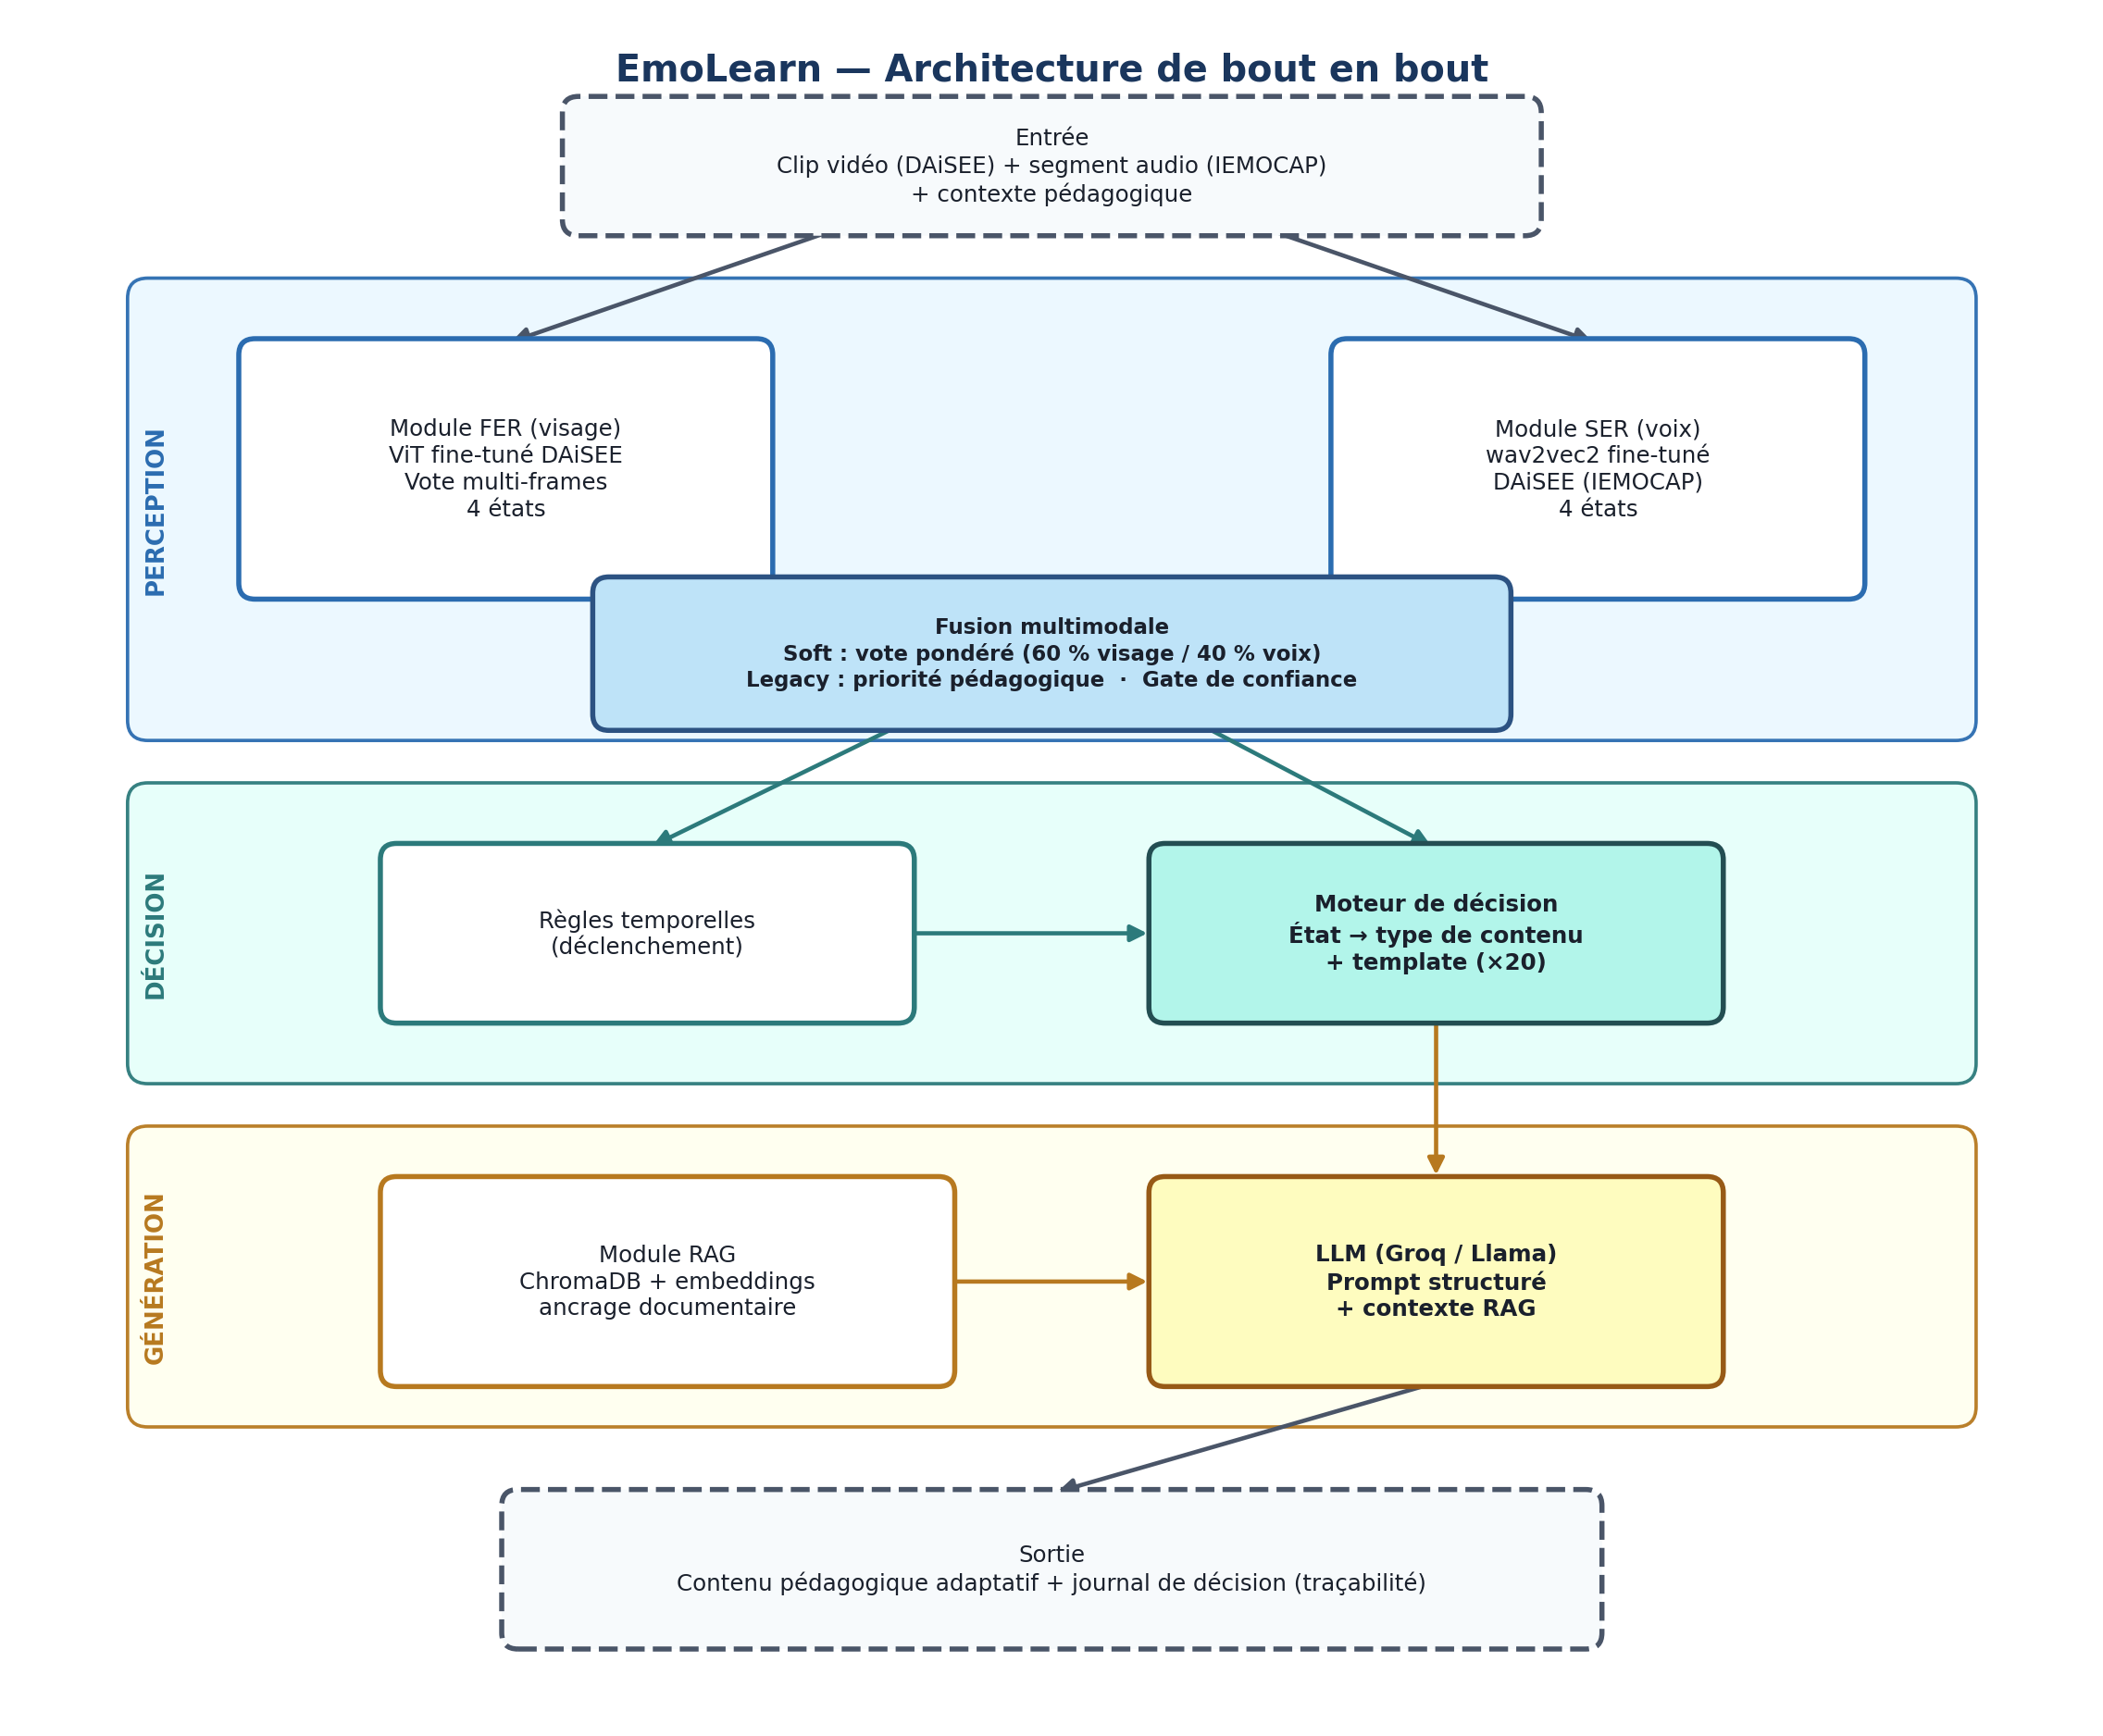
\includegraphics[width=1\textwidth]{figures/emolearn_architecture.png}
\caption{Architecture en couches d'\emolearn{}.}
\label{fig:architecture}
\end{figure}

\subsection{Workflow de génération adaptative}
\label{subsec:workflow}

Le traitement d'un clip suit un enchaînement déterministe de sept étapes.

\begin{enumerate}[label=\textbf{\arabic*.}]
  \item \textbf{Acquisition.} Le fichier vidéo du clip \textsc{DAiSEE} est
  résolu sur disque, puis associé au segment audio apparié et à un contexte
  pédagogique (concept, module, niveau, moment du cours).
  \item \textbf{Perception par modalité.} Le module FER traite \emph{uniquement}
  le visage : il détecte le visage sur plusieurs images du clip, agrège les
  distributions par vote multi-frames, et estime l'état facial. En parallèle,
  le module SER traite \emph{uniquement} la voix et estime l'état vocal. Chaque
  module reste donc séparé (une modalité = un estimateur) ; ce n'est qu'à
  l'étape suivante que les deux sorties sont combinées.
  \item \textbf{Fusion.} Les deux estimations sont combinées
  (pondération $w_v = 0{,}6$ / $w_a = 0{,}4$) et les conflits sont résolus
  (section~\ref{sec:perception}).
  \item \textbf{Analyse temporelle.} L'historique récent des clips décide de
  l'urgence et du déclenchement.
  \item \textbf{Décision.} Si une intervention est requise, le moteur
  détermine la stratégie, le type de contenu et le patron (A1--D5).
  \item \textbf{Génération.} Un prompt structuré est construit, éventuellement
  enrichi par le RAG, puis soumis au LLM.
  \item \textbf{Restitution et traçabilité.} Le contenu est renvoyé à
  l'interface ; chaque décision est journalisée (état, stratégie, patron,
  paramètres de fusion).
\end{enumerate}

Lorsque l'analyse temporelle conclut à un engagement stable, aucune génération
n'est déclenchée : le système signale une \emph{non-intervention}. Ce choix
évite de sur-solliciter l'apprenant et documente le choix de ne rien faire.

\paragraph{Perception sur le signal, annotations réservées à la vérité terrain.}
La couche de perception opère sur le \textbf{signal brut} et non sur les
annotations du corpus. Le module FER ouvre le fichier vidéo, y détecte le
visage et produit ses propres distributions ; le module SER analyse la forme
d'onde. Les niveaux annotés dans \textsc{DAiSEE} tiennent exclusivement le
rôle d'\textbf{étiquettes de référence}, pour l'entraînement des mappings
appris (section~\ref{sec:perception}) et pour la validation. Un système qui
lirait les annotations pour \emph{estimer} l'état n'évaluerait que lui-même.

%==============================================================================
\section{Analyse du dataset DAiSEE}
\label{sec:daisee}

\subsection{Description et caractéristiques}

Le corpus \textsc{DAiSEE} (\emph{Dataset for Affective States in
E-Environments}) \cite{gupta2016daisee} est un jeu de données vidéo de
référence pour la reconnaissance de l'engagement \og dans la nature \fg{}
(\emph{in the wild}). Il rassemble environ 9\,000 clips d'une dizaine de
secondes, capturés auprès d'étudiants en situation réelle d'apprentissage en
ligne, dans des conditions variées d'éclairage et d'arrière-plan. Chaque clip
est annoté selon \textbf{quatre états affectifs} (l'ennui
(\emph{boredom}), la confusion, l'engagement et la frustration), chacun
exprimé sur une échelle ordinale à \textbf{quatre niveaux d'intensité}
(0~: très faible, 1~: faible, 2~: élevé, 3~: très élevé). Le
tableau~\ref{tab:daisee-etats} synthétise cette taxonomie, qui constitue le
référentiel de tout le projet. Elle est plus opératoire, pour un apprenant
silencieux devant une vidéo, que les cadres CoI ou ICAP discutés au
chapitre~\ref{chap:etat_art}, conçus pour le codage de forums.

\begin{table}[H]
\centering
\renewcommand{\arraystretch}{1.2}
\begin{tabular}{|>{\bfseries}l|p{9.5cm}|}
\hline
\rowcolor{gray!20}
État & Signification dans le contexte d'apprentissage \\
\hline
Engagement  & Attention active et implication dans la tâche d'apprentissage. \\
\hline
Boredom     & Ennui, désengagement passif, baisse de la stimulation. \\
\hline
Confusion   & Incompréhension d'un concept, difficulté de traitement. \\
\hline
Frustration & Blocage émotionnel, tension liée à une difficulté persistante. \\
\hline
\end{tabular}
\caption{Les quatre états affectifs annotés dans \textsc{DAiSEE}
(niveaux d'intensité 0 à 3).}
\label{tab:daisee-etats}
\end{table}

Chaque enregistrement est identifié par un \texttt{ClipID} et associé à un
quadruplet de scores
$s = (s_{\mathrm{B}}, s_{\mathrm{C}}, s_{\mathrm{E}}, s_{\mathrm{F}})
\in \{0,1,2,3\}^4$.
L'\textbf{état dominant} d'un clip est
\begin{equation}
  e^{\star} \;=\; \arg\max_{e \in E} s_e,
  \label{eq:etat-dominant}
\end{equation}
où $E = \{\text{Boredom}, \text{Confusion}, \text{Engagement},
\text{Frustration}\}$. En cas d'égalité, un départage pédagogique s'applique :
Frustration $>$ Confusion $>$ Boredom $>$ Engagement. Cette règle
garantit qu'un apprenant en difficulté n'est jamais classé \og engagé \fg{}
par simple ex-\ae{}quo : mieux vaut signaler une frustration que la masquer
derrière un engagement concurrent.

\subsection{Distribution des états d'engagement}

L'analyse des annotations révèle un \textbf{déséquilibre de classes marqué},
caractéristique documentée de \textsc{DAiSEE}. L'engagement est largement
dominant (niveaux 2 ou 3), tandis que la confusion et surtout la frustration
intenses sont rares. Deux conséquences en découlent pour la conception :

\begin{itemize}[leftmargin=1.4em]
  \item les états \emph{critiques} (confusion et frustration élevées),
  pourtant les plus importants pédagogiquement, sont \textbf{sous-représentés} ;
  \item maximiser l'exactitude globale tendrait à privilégier la classe
  majoritaire au détriment des états à risque.
\end{itemize}

Ce constat justifie d'accorder une \textbf{priorité pédagogique} aux états
négatifs dans la fusion et la décision (section~\ref{sec:modele}). La
figure~\ref{fig:distribution} restitue la distribution observée.

\begin{figure}[H]
\centering
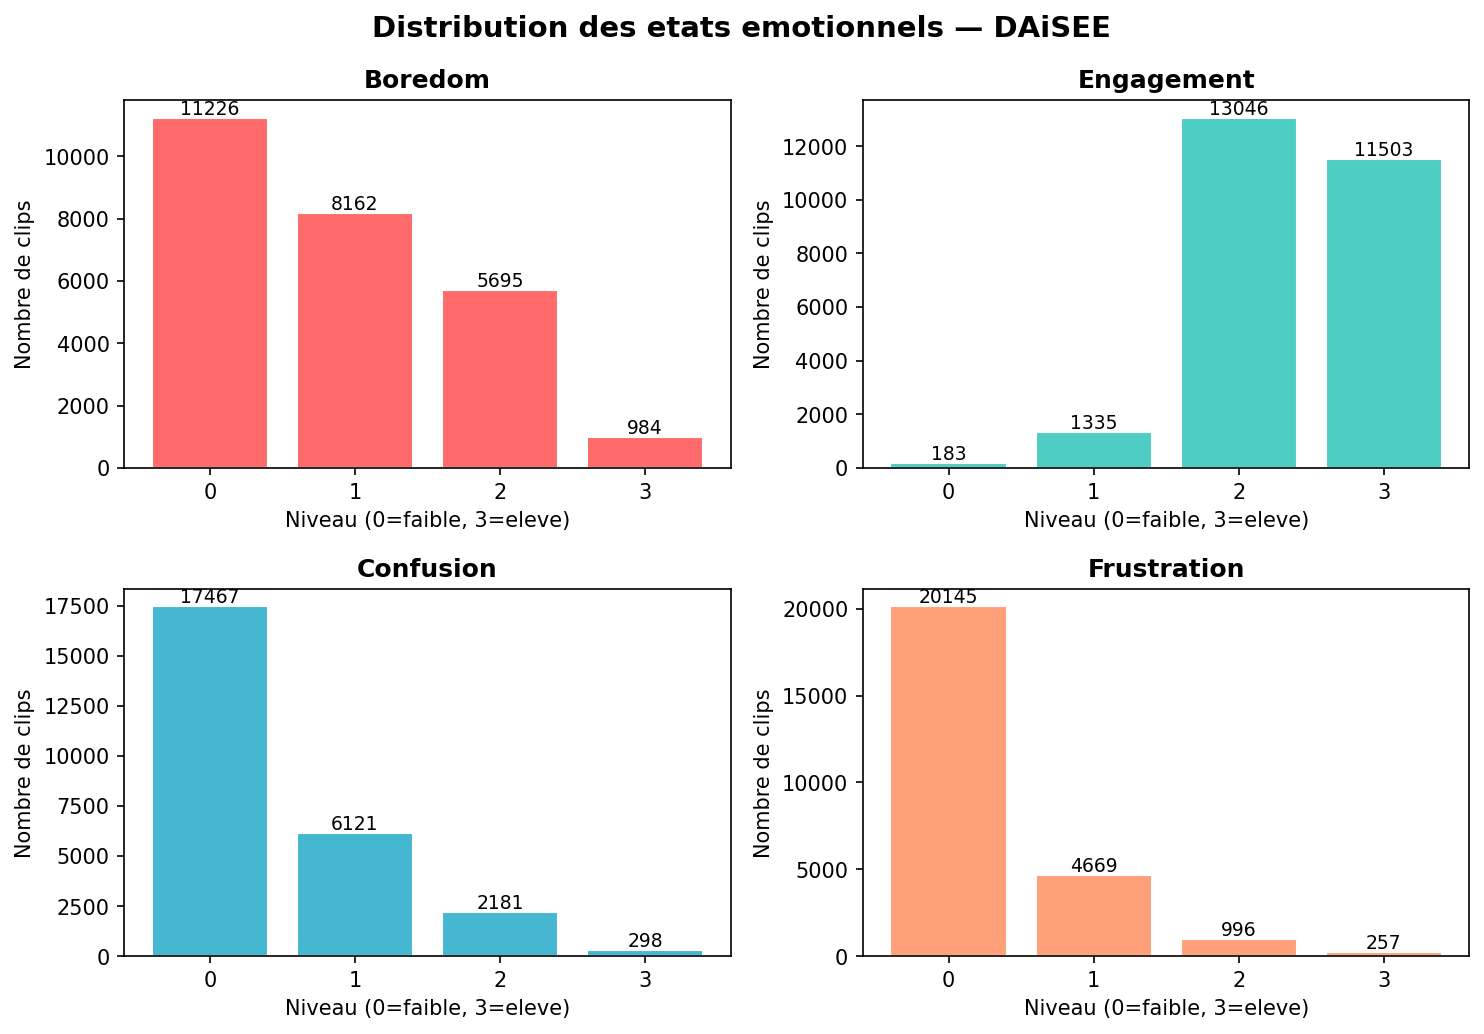
\includegraphics[width=0.9\textwidth]{figures/daisee_distribution.png}
\caption{Distribution des états d'engagement dans \textsc{DAiSEE}
(ensemble des partitions annotées du corpus).}
\label{fig:distribution}
\end{figure}

\subsection{Analyse exploratoire des données}

L'analyse exploratoire poursuit trois objectifs. Premièrement,
\textbf{caractériser les co-occurrences} : l'engagement varie en sens inverse
de l'ennui, tandis que confusion et frustration tendent à coexister. Deuxièmement,
\textbf{déterminer l'état dominant} de chaque clip via
l'équation~\eqref{eq:etat-dominant}. Troisièmement, \textbf{constituer un
sous-ensemble représentatif} : une sélection de scénarios (clips isolés) et
de parcours (séquences) alimente la simulation.

\subsection{Identification de patterns critiques}

Au-delà de l'état instantané, la conception introduit un \textbf{pattern
pédagogique} qui qualifie la situation globale d'un clip ou d'une séquence
et oriente le choix du patron de génération
(tableau~\ref{tab:patterns}).

\begin{table}[H]
\centering
\renewcommand{\arraystretch}{1.2}
\begin{tabular}{|>{\bfseries}l|p{9.2cm}|}
\hline
\rowcolor{gray!20}
Pattern & Condition (scores DAiSEE) \\
\hline
critique          & Au moins trois états simultanément $\geq 2$ (situation cumulée). \\
\hline
engagement\_faible & Engagement $\leq 1$, sans confusion ni frustration marquées. \\
\hline
confusion         & État dominant = Confusion. \\
\hline
ennui\_eleve       & État dominant = Boredom. \\
\hline
frustration       & État dominant = Frustration. \\
\hline
stable            & Engagement dominant, situation acceptable. \\
\hline
\end{tabular}
\caption{Patterns pédagogiques dérivés des scores DAiSEE.}
\label{tab:patterns}
\end{table}

%==============================================================================
\section{Positionnement et usage du corpus IEMOCAP}
\label{sec:iemocap}

\textsc{IEMOCAP} (\emph{Interactive Emotional Dyadic Motion Capture})
\cite{busso2008iemocap} constitue le \textbf{second jeu de données} mobilisé.
Contrairement à \textsc{DAiSEE}, il ne fonde pas la taxonomie pédagogique :
il apporte la \textbf{modalité vocale} et, dans un cadre distinct, un
\textbf{sous-corpus audiovisuel aligné} pour valider la fusion.

\subsection{Complémentarité avec \textsc{DAiSEE}}

Les deux corpus couvrent des contextes distincts, mais convergent vers la
même taxonomie à quatre états (tableau~\ref{tab:complementarite-corpus}).
Cette complémentarité répond à la lacune \og signal \fg{} du
chapitre~\ref{chap:etat_art} : fusionner visage \emph{et} voix, plutôt que
le seul canal visuel.

\begin{table}[H]
\centering
\renewcommand{\arraystretch}{1.2}
\begin{tabular}{|>{\bfseries}l|p{4.95cm}|p{4.95cm}|}
\hline
\rowcolor{gray!20}
Aspect & \textsc{DAiSEE} & \textsc{IEMOCAP} \\
\hline
Contexte & Apprenants en e-learning (\emph{in the wild}) &
Dialogues actés, dyades (sessions 1--5) \\
\hline
Modalité principale & Visage / engagement annoté &
Voix (+ vidéo pour le banc d'essai) \\
\hline
Étiquettes natives & 4 états $\times$ niveaux 0--3 &
Émotions discrètes + dimensions VAD \\
\hline
Rôle dans \emolearn{} &
Socle : scénarios, patterns, décision &
Voix en production ; validation AV alignée \\
\hline
\end{tabular}
\caption{Complémentarité des corpus \textsc{DAiSEE} et \textsc{IEMOCAP} dans
\emolearn{}.}
\label{tab:complementarite-corpus}
\end{table}

\subsection{Description et caractéristiques}

\textsc{IEMOCAP} rassemble des enregistrements audiovisuels de dialogues
entre deux acteurs, annotés au niveau de l'\emph{utterance} par des émotions
discrètes et par des scores valence--activation--dominance (VAD). Le corpus
parsé du projet compte 10\,039 utterances, chacune associée à un fichier
audio réel. Les annotations sont consommées par le module SER
(section~\ref{subsec:ser-appris}).

\subsection{Projection des émotions vers la taxonomie \textsc{DAiSEE}}
\label{subsec:mapping-iemocap}

Les émotions conversationnelles d'\textsc{IEMOCAP} ne coïncident pas
naturellement avec les états d'engagement de \textsc{DAiSEE}. La conception
retient donc une \textbf{table de projection}
(tableau~\ref{tab:mapping-iemocap}). Cette correspondance est une
\textbf{hypothèse de construit}, et non une équivalence psychologique
démontrée : elle rend le pipeline cohérent en ramenant visage et voix dans
un espace commun, mais elle doit être mesurée
(section~\ref{subsec:sensibilite-mapping}).

\begin{table}[H]
\centering
\renewcommand{\arraystretch}{1.15}
\begin{tabular}{|>{\bfseries}l|l|c|p{4.8cm}|}
\hline
\rowcolor{gray!20}
Code IEMOCAP & État DAiSEE & Niv. & Justification pédagogique \\
\hline
hap, exc & Engagement  & 3 & Valence positive, activation forte \\
\hline
neu      & Boredom     & 1 & Neutre prolongé $\approx$ faible stimulation \\
\hline
sad      & Boredom     & 2 & Faible engagement \\
\hline
ang, fru & Frustration & 3 & Blocage, tension \\
\hline
dis      & Frustration & 2 & Rejet, gêne modérée \\
\hline
sur, fea & Confusion   & 2--3 & Incertitude, surprise cognitive \\
\hline
xxx      & Boredom     & 1 & Non classifié $\rightarrow$ défaut prudent \\
\hline
\end{tabular}
\caption{Projection de référence des émotions \textsc{IEMOCAP} vers la taxonomie
\textsc{DAiSEE} (hypothèse de travail).}
\label{tab:mapping-iemocap}
\end{table}

\subsection{Appariement voix--scénarios dans le pipeline produit}
\label{subsec:appariement}

Dans la chaîne de \textbf{production} (simulation sur clips \textsc{DAiSEE}),
le visage et la voix ne proviennent pas du même individu : le FER analyse un
clip \textsc{DAiSEE}, le SER sélectionne une utterance \textsc{IEMOCAP}
\emph{émotionnellement cohérente} avec l'état dominant du scénario. La règle
est la suivante :
\begin{enumerate}[label=\textbf{\arabic*.}, leftmargin=1.6em]
  \item calcul de l'état dominant du scénario \textsc{DAiSEE}
        (équation~\eqref{eq:etat-dominant}) ;
  \item filtrage des utterances projetées sur le \emph{même} état ;
  \item sélection reproductible via l'identifiant du scénario
        (\texttt{scenario\_id} modulo la taille du pool) ;
  \item analyse du segment audio réel sur l'intervalle annoté.
\end{enumerate}

Cet appariement améliore la cohérence émotionnelle par rapport à un tirage
aléatoire, mais conserve une limite assumée : \textbf{absence de
synchronisation temporelle} entre l'apprenant filmé et le locuteur
enregistré. Cette tension n'est levée que dans le banc d'essai ci-dessous.

\subsection{Sous-corpus audiovisuel aligné (Option~A)}
\label{subsec:option-a}

Pour \textbf{valider la fusion} sans l'appariement hétérogène, un sous-corpus
\textsc{IEMOCAP} \textbf{audiovisuel aligné} est construit hors ligne : pour
chaque utterance, le visage et la voix proviennent du \textbf{même locuteur},
synchronisés sur le segment annoté. Les vidéos dyadiques imposent un crop
(moitié gauche ou droite selon les marqueurs mocap). Ce banc d'essai
partage le \textbf{même moteur de fusion} que la production ; seules les
entrées changent. Les métriques comparatives sont présentées au
chapitre~\ref{chap:validation}.

\subsection{Analyse de sensibilité du mapping}
\label{subsec:sensibilite-mapping}

La robustesse de la projection émotion\,$\rightarrow$\,engagement est évaluée
par une \textbf{analyse de sensibilité} sur les 10\,039 utterances
(tableau~\ref{tab:sensibilite-mapping}). Les variantes affectant
\texttt{neu} (neutre $\rightarrow$ Engagement) ou \texttt{sad} (tristesse
$\rightarrow$ Frustration) modifient jusqu'à 17\,\% et 10,8\,\% des
étiquettes projetées, confirmant que l'hypothèse n'est pas anodine. Le
protocole et la discussion sont détaillés au
chapitre~\ref{chap:validation}.

\begin{table}[H]
\centering
\small
\renewcommand{\arraystretch}{1.2}
\begin{tabular}{|>{\bfseries}l|p{6.4cm}|r|}
\hline
\rowcolor{gray!20}
Variante testée & Modification du mapping & Utterances \\
\hline
neu\_engagement &
\texttt{neu} $\rightarrow$ Engagement (au lieu de Boredom) & 17,0\,\% \\
\hline
sad\_frustration &
\texttt{sad} $\rightarrow$ Frustration (au lieu de Boredom) & 10,8\,\% \\
\hline
surprise\_engagement &
\texttt{sur} $\rightarrow$ Engagement (au lieu de Confusion) & 1,1\,\% \\
\hline
disgust\_boredom &
\texttt{dis} $\rightarrow$ Boredom (au lieu de Frustration) & 0,0\,\% \\
\hline
\end{tabular}
\caption{Sensibilité du mapping \textsc{IEMOCAP} $\rightarrow$ \textsc{DAiSEE}
(sur 10\,039 utterances).}
\label{tab:sensibilite-mapping}
\end{table}

%==============================================================================
\section{Couche de perception}
\label{sec:perception}

La perception transforme un couple (vidéo, audio) en une distribution sur
$E$ et en un couple $(\hat{e}, \hat{n})$ (état et niveau). Chaque modalité
dispose d'une \emph{référence explicable} et d'une \emph{variante fine-tunée} ;
la fusion existe en deux familles aux objectifs distincts.

\subsection{Taxonomie des états et mapping facial de référence}

Les émotions produites par les modules FER (sept classes) et SER sont
d'abord ramenées dans l'espace \textsc{DAiSEE}. Cette mise en correspondance
est conçue à \textbf{deux niveaux} : une table fixe, justifiable
\emph{a priori} (tableau~\ref{tab:fer-mapping}) ; et un modèle
\emph{appris} qui la remplace lorsqu'il apporte un gain mesuré.

\begin{table}[H]
\centering
\renewcommand{\arraystretch}{1.15}
\begin{tabular}{|>{\bfseries}l|l|c|}
\hline
\rowcolor{gray!20}
Émotion faciale & État DAiSEE & Niveau associé \\
\hline
happy    & Engagement  & 3 \\
\hline
neutral  & Boredom     & 1 \\
\hline
sad      & Boredom     & 2 \\
\hline
angry    & Frustration & 3 \\
\hline
fear     & Confusion   & 3 \\
\hline
surprise & Confusion   & 2 \\
\hline
disgust  & Frustration & 2 \\
\hline
\end{tabular}
\caption{Mapping heuristique de référence des émotions faciales (FER) vers les
états DAiSEE.}
\label{tab:fer-mapping}
\end{table}

\subsection{Perception faciale : mapping, classifieur et fine-tuning ViT}
\label{subsec:fer-appris}

La table~\ref{tab:fer-mapping} traduit un raisonnement pédagogique (un
visage en colère signale une frustration, un visage neutre l'amorce d'un
désengagement) mais elle n'est calibrée sur aucune donnée. La conception
prévoit donc plusieurs niveaux, du plus transparent au plus performant.

Le premier niveau appris, volontairement \emph{léger}, laisse le réseau de
reconnaissance faciale pré-entraîné inchangé et n'apprend que le lien entre
ses sept scores d'émotion et la taxonomie d'engagement. Un
\textbf{Random Forest} est entraîné sur ce couple (étiquettes
\textsc{DAiSEE}), avec sélection d'hyperparamètres par validation croisée
stratifiée. Un garde-fou peut conditionner l'usage de ce mapping à un gain
simultané d'exactitude et de F-score macro, afin d'éviter un classifieur
biaisé vers Engagement.

Le mode retenu \textbf{par défaut en production} va plus loin : un
\textbf{Vision Transformer} (ViT) \cite{dosovitskiy2021vit} est \textbf{fine-tuné} de bout en bout vers
les quatre états \textsc{DAiSEE}, à partir d'un modèle pré-entraîné
d'émotions faciales. Le runtime agrège plusieurs frames du clip (moyenne des
probabilités, avec rejet des frames peu confiantes). Ce choix élimine le
détour par les sept émotions génériques et produit directement une
distribution $P_{\mathrm{visage}}(e)$ sur $E$.

Les modes demeurent interchangeables par configuration : mapping
heuristique, Random Forest, ou ViT fine-tuné (défaut). La
table~\ref{tab:fer-mapping} conserve le statut de \textbf{baseline}.

\subsection{Perception vocale : heuristique acoustique et fine-tuning wav2vec2}
\label{subsec:ser-appris}

Le module vocal suit la même logique. La \textbf{méthode heuristique} sert
de référence : elle extrait des descripteurs acoustiques classiques (énergie,
taux de passage par zéro, centroïde spectral, $F_0$) puis applique des
seuils dans l'espace valence--activation--dominance, avant projection vers
\textsc{DAiSEE}. Entièrement transparente, elle reste grossière.

La \textbf{méthode apprise}, retenue par défaut, part d'un encodeur
wav2vec2 \cite{baevski2020wav2vec2} déjà spécialisé pour la reconnaissance
d'émotions, \textbf{fine-tuné} vers les quatre états \textsc{DAiSEE}
(\emph{full fine-tuning}). Ce choix répond à une contrainte précise : le
modèle de base ne possède aucune classe \textbf{Confusion}. Le fine-tuning
sur des étiquettes projetées (surprise et peur alimentant Confusion)
fait émerger cette classe absente. Une pondération de classes compense le
déséquilibre. L'heuristique sert de repli lorsque le modèle n'est pas
disponible.

\subsection{Fusion multimodale : formalisation}
\label{subsec:fusion-math}

Soit $P_v(e)$ et $P_a(e)$ les distributions produites par le visage et la
voix, et $w_v \in [0,1]$ le poids du visage ($w_a = 1 - w_v$). Deux familles
de fusion sont conservées.

\paragraph{Famille \emph{weighted vote} (défaut produit).}
La pondération porte sur l'état lui-même :
\begin{equation}
  \hat{P}(e) \;=\; w_v \, P_v(e) \;+\; (1-w_v)\, P_a(e),
  \qquad
  \hat{e} \;=\; \arg\max_{e \in E} \hat{P}(e).
  \label{eq:vote}
\end{equation}
Un \emph{gate} de fiabilité annule le poids d'une modalité dont le score de
confiance est inférieur à un seuil $\theta$ (défaut $0{,}40$). Si les deux
modalités sont sous le seuil, un repli de priorité pédagogique s'applique.
Si la voix est absente, \eqref{eq:vote} se réduit à $P_v$.

\paragraph{Famille \emph{pedagogical priority} (legacy).}
Chaque modalité décide d'abord un état $(e_v, n_v)$ et $(e_a, n_a)$. Si
$e_v = e_a$, le niveau fusionné est la moyenne pondérée
\begin{equation}
  \hat{n} \;=\; \mathrm{round}\bigl( w_v \, n_v + (1-w_v)\, n_a \bigr).
  \label{eq:niveau}
\end{equation}
Si $e_v \neq e_a$, l'état retenu est celui de priorité maximale
\begin{equation}
  \pi(\text{Frustration}) > \pi(\text{Confusion})
  > \pi(\text{Boredom}) > \pi(\text{Engagement}),
  \label{eq:priorite}
\end{equation}
indépendamment de $w_v$. Dans cette formulation, \textbf{le poids des
modalités n'influence pas l'état} : il ne pondère que le niveau. C'est
précisément ce que la famille par vote corrige.

Le tableau~\ref{tab:conflits} résume la gestion des conflits dans la famille
legacy ; le tableau~\ref{tab:familles-fusion} compare les deux objectifs.

\begin{table}[H]
\centering
\renewcommand{\arraystretch}{1.2}
\begin{tabular}{|>{\bfseries}l|p{8.8cm}|}
\hline
\rowcolor{gray!20}
Type de conflit & Résolution \\
\hline
Accord parfait / partiel & Fusion pondérée normale ($w_v = 0{,}6$). \\
\hline
Conflit de niveau        & Moyenne pondérée des niveaux (même état). \\
\hline
Conflit mineur           & Modalité au score de confiance le plus élevé. \\
\hline
Conflit modéré / majeur  & \emph{Pedagogical priority} (défaut) ou \emph{confidence}. \\
\hline
\end{tabular}
\caption{Gestion des conflits dans la fusion multimodale (famille legacy).}
\label{tab:conflits}
\end{table}

\subsection{Les deux familles de fusion}
\label{subsec:vote}

Les deux familles ne poursuivent pas le même objectif et sont donc
conservées, sélectionnables par configuration. La fusion par priorité
pédagogique est volontairement asymétrique : elle accepte de se tromper au
profit de l'état le plus grave. La fusion par vote est symétrique et vise
l'exactitude. Le chapitre~\ref{chap:validation} mesure l'arbitrage.

\begin{table}[H]
\centering
\renewcommand{\arraystretch}{1.2}
\begin{tabular}{|>{\bfseries}l|>{\raggedright\arraybackslash}p{4.4cm}|>{\raggedright\arraybackslash}p{4.4cm}|}
\hline
\rowcolor{gray!20}
Famille & Ce que pondère $w_v$ & Objectif optimisé \\
\hline
\emph{Pedagogical priority} & Le niveau d'intensité ; l'état suit~\eqref{eq:priorite} &
Rappel des états critiques (sécurité pédagogique) \\
\hline
\emph{Weighted vote} & L'état lui-même, via~\eqref{eq:vote} &
Exactitude de la décision \\
\hline
\end{tabular}
\caption{Les deux familles de fusion et leurs objectifs respectifs.}
\label{tab:familles-fusion}
\end{table}

\paragraph{Choix des poids.}
La valeur $w_v = 0{,}6$ traduit d'abord une hypothèse (le visage est la
modalité native de \textsc{DAiSEE}), puis fait l'objet d'un balayage
empirique de $0{,}5$ à $0{,}9$ (chapitre~\ref{chap:validation}). Le poids
n'a d'effet sur l'état que dans la variante par vote ; $0{,}6/0{,}4$
maximise le rappel des états urgents, conformément à la priorité posée en
section~\ref{sec:daisee}.

%==============================================================================
\section{Modèle engagement-adaptation}
\label{sec:modele}

Le modèle engagement\,$\rightarrow$\,adaptation constitue le c\oe ur
scientifique du framework. Il transforme l'état perçu $(\hat{e}, \hat{n})$
et l'historique $H$ en une décision pédagogique traçable : un type de
contenu, un patron et un déclenchement. C'est la réponse à la lacune
\og décision \fg{} du chapitre~\ref{chap:etat_art} : des règles
\emph{explicites}, journalisées, plutôt qu'un réglage opaque de style.

\subsection{Formulation}

Soit $H = (s^{(t-k)}, \ldots, s^{(t)})$ l'historique des $k$ derniers
quadruplet de scores dérivés de la fusion. Le moteur calcule
\begin{equation}
  \bigl(\tau,\, \gamma,\, u\bigr)
  \;=\;
  \Delta\bigl(\hat{e},\, \hat{n},\, s^{(t)},\, H\bigr),
  \label{eq:decision}
\end{equation}
où $\tau \in \{A,B,C,D,A{+}D,D{+}A,\varnothing\}$ est le type de contenu,
$\gamma \in \{A1,\ldots,D5\}$ le patron, et
$u \in \{\text{immédiate}, \text{rapide}, \text{différée}, \text{aucune}\}$
l'urgence. La fonction $\Delta$ est une cascade de règles, non un réseau :
chaque sortie est inspectable.

Les scores $s^{(t)}$ utilisés par $\Delta$ sont \textbf{dérivés de la
fusion}, et non lus dans les annotations \textsc{DAiSEE}. Si la fusion
expose $\hat{P}$, chaque dimension est projetée sur $\{0,1,2,3\}$ par
$s_e = \mathrm{round}(3\,\hat{P}(e))$ ; sinon, l'état retenu reçoit le
niveau fusionné et les autres dimensions valent 0.

\subsection{Mapping états vers besoins pédagogiques}

Quatre types fondamentaux sont définis, plus deux composites :

\begin{description}[leftmargin=2.2em]
  \item[Type A : Explication.] Reformuler un concept mal compris.
  \item[Type B : Exemple.] Ancrer le concept dans une application concrète.
  \item[Type C : Exercice.] Approfondir par un défi adapté au niveau.
  \item[Type D : Encouragement.] Apporter un soutien émotionnel.
  \item[Type A+D / D+A : Composites.] Combiner explication et soutien
  lorsque confusion et frustration coexistent.
\end{description}

Le mapping est un ensemble de règles ordonnées, appliquées par priorité
décroissante d'urgence (tableau~\ref{tab:mapping}). La première règle
satisfaite l'emporte.

\begin{table}[H]
\centering
\small
\renewcommand{\arraystretch}{1.25}
\begin{tabular}{|c|p{5.1cm}|>{\bfseries}c|>{\raggedright\arraybackslash}p{4.3cm}|}
\hline
\rowcolor{gray!20}
Ordre & Condition (scores DAiSEE) & Type & Stratégie \\
\hline
1 & Confusion $\geq 3$ \textbf{et} Frustration $\geq 2$ & A+D & Aide de déblocage immédiate \\
\hline
2 & Engagement $= 0$                                    & B   & Réengagement urgent \\
\hline
3 & Frustration $\geq 2$                                & D+A & Encouragement + simplification \\
\hline
4 & Confusion $\geq 2$                                  & A   & Explication alternative \\
\hline
5 & Boredom $\geq 2$                                    & C   & Exercice avancé \\
\hline
6 & Engagement $\leq 1$                                 & B   & Exemple concret stimulant \\
\hline
7 & Boredom $= 1$                                       & B   & Application pratique \\
\hline
8 & Engagement $\geq 2$                                 & D   & Renforcement positif \\
\hline
9 & Sinon                                               & -- & Continuation normale (pas d'adaptation) \\
\hline
\end{tabular}
\caption{Règles de mapping engagement $\rightarrow$ type de contenu et stratégie.}
\label{tab:mapping}
\end{table}

Cette ordonnance suit une logique pédagogique simple : un contenu trop dense
(confusion) appelle une simplification ; un contenu sous-stimulant (ennui)
appelle un défi ; un blocage (frustration) appelle d'abord un soutien, non
un exercice supplémentaire. Les fondements théoriques correspondants
(charge cognitive, dynamique affect--apprentissage) sont exposés aux
chapitres~\ref{chap:fondements} et~\ref{chap:etat_art}.

\subsection{Règles de déclenchement d'adaptation}

La décision d'intervenir ne repose pas uniquement sur le clip courant mais
sur sa \textbf{dynamique temporelle}. Un module dédié classe la situation
selon quatre niveaux d'urgence (tableau~\ref{tab:temporel}). Cette
temporalisation évite deux écueils : réagir à un signal isolé, et laisser
s'installer un état négatif durable.

\begin{table}[H]
\centering
\renewcommand{\arraystretch}{1.2}
\begin{tabular}{|>{\bfseries}l|p{8.6cm}|}
\hline
\rowcolor{gray!20}
Urgence & Règle de déclenchement \\
\hline
Immédiate & Confusion $\geq 3$ et Frustration $\geq 2$ sur le clip courant ; ou Engagement $= 0$. \\
\hline
Rapide    & Boredom, Confusion ou Frustration $\geq 2$ sur 2 clips consécutifs. \\
\hline
Différée  & Engagement $\leq 1$ (ou Boredom $= 1$) stable sur 4 clips. \\
\hline
Aucune    & Engagement $\geq 2$ stable sur 2 clips $\rightarrow$ pas d'intervention. \\
\hline
\end{tabular}
\caption{Règles temporelles de déclenchement de l'adaptation.}
\label{tab:temporel}
\end{table}

Si $u = \text{aucune}$, alors $\tau = \varnothing$ : le système n'appelle
pas le LLM.

\subsection{Stratégies pédagogiques par état}

En synthèse, chaque état dominant est associé à une famille de stratégies :
à la \emph{confusion} répond l'explication (A) ; à l'\emph{ennui} l'exemple
(B) ou l'exercice (C) selon que l'engagement est faible ou que la maîtrise
est déjà installée ; à la \emph{frustration} le soutien (D), combiné à une
simplification en cas de confusion associée ; un \emph{bon engagement}
appelle un renforcement positif (D) destiné à entretenir la dynamique.

%==============================================================================
\section{Système de génération}
\label{sec:generation}

\subsection{Architecture de prompting contextuel}

Une fois le patron $\gamma$ sélectionné, la génération repose sur une
\textbf{ingénierie de prompt} structurée. Le prompt est organisé en blocs
explicites : un contexte de référence issu du RAG (optionnel), un bloc
\textbf{[Contexte pédagogique]} (sujet, module, concept, niveau, objectif),
un bloc \textbf{[État d'engagement]} (état, intensité, durée, pattern,
moment du cours), un bloc \textbf{[Tâche]} (patron et objectif), un bloc
\textbf{[Contraintes]} (longueur, format, ton) et un bloc
\textbf{[Instructions spécifiques]} propre au patron. Un \emph{message
système} fixe le rôle (expert en pédagogie) et impose de s'appuyer
uniquement sur le contexte fourni, afin de limiter les hallucinations.
La génération est assurée par un LLM de la famille \textsc{LLaMA}~3.1
\cite{dubey2024llama3} servi via API, avec une température basse ($0{,}3$)
privilégiant la stabilité.

\subsection{Typologie du contenu adaptatif}

Les patrons se répartissent selon les quatre types, chaque type portant un
objectif et un registre de ton distincts (tableau~\ref{tab:typologie}).

\begin{table}[H]
\centering
\renewcommand{\arraystretch}{1.2}
\begin{tabular}{|>{\bfseries}c|l|l|}
\hline
\rowcolor{gray!20}
Type & Objectif dominant & Registre / ton \\
\hline
A   & Clarifier, débloquer   & Rassurant, patient, pédagogue \\
\hline
B   & Stimuler, contextualiser & Dynamique, concret, motivant \\
\hline
C   & Approfondir, consolider & Challengeant, structurant \\
\hline
D   & Encourager, renforcer  & Empathique, valorisant \\
\hline
\end{tabular}
\caption{Typologie des contenus adaptatifs par famille de patrons.}
\label{tab:typologie}
\end{table}

\subsection{Templates de prompts structurés}

Le système propose une bibliothèque de \textbf{vingt patrons}
(A1--A5, B1--B5, C1--C5, D1--D5). Chaque patron définit un format, un ton,
une longueur cible et un jeu d'instructions. Cette bibliothèque constitue
une contribution centrale de la conception : elle conditionne la génération
par l'état, plutôt que par un simple réglage de style ou de difficulté.

{\small
\begin{longtable}{|>{\bfseries}c|l|l|c|}
\caption{Bibliothèque des 20 patrons de prompts structurés (A1--D5).}
\label{tab:templates}\\
\hline
\rowcolor{gray!20}
ID & Description & Format / ton & Long. \\
\hline
\endfirsthead
\multicolumn{4}{l}{\footnotesize\itshape Suite du tableau~\ref{tab:templates}}\\
\hline
\rowcolor{gray!20}
ID & Description & Format / ton & Long. \\
\hline
\endhead
\hline
\endfoot
\hline
\endlastfoot
A1 & Explication alternative : confusion modérée & Étapes / rassurant & 200 \\
\hline
A2 & Micro-explication : confusion intense & Décomposé / patient & 150 \\
\hline
A3 & Aide de déblocage : confusion + frustration & Déblocage / empathique & 200 \\
\hline
A4 & Explication de fond : confusion récurrente & Fond / stratégique & 250 \\
\hline
A5 & Explication narrative : concept abstrait & Narratif / créatif & 200 \\
\hline
B1 & Exemple concret : ennui modéré & Engageant / dynamique & 200 \\
\hline
B2 & Cas pratique : engagement faible & Cas / curiosité & 250 \\
\hline
B3 & Mise en pratique : ennui après théorie & Action / pratique & 200 \\
\hline
B4 & Application réelle : contextualisation & Pro / carrière & 250 \\
\hline
B5 & Exemple interdisciplinaire & Transversal / créatif & 200 \\
\hline
C1 & Exercice avancé : ennui élevé (maîtrise) & Structuré / challengeant & 250 \\
\hline
C2 & Exercice de consolidation & Progressif / encourageant & 200 \\
\hline
C3 & Exercice créatif & Ouvert / valorisant & 200 \\
\hline
C4 & Mini-projet & Projet / ambitieux & 250 \\
\hline
C5 & Exercice comparatif & Analytique / critique & 200 \\
\hline
D1 & Encouragement : frustration modérée & Motivant / empathique & 150 \\
\hline
D2 & Soutien : frustration élevée & Soutien / déstressant & 180 \\
\hline
D3 & Remotivation : découragement & Remotivant / recentrant & 200 \\
\hline
D4 & Renforcement positif : bon engagement & Positif / valorisant & 150 \\
\hline
D5 & Félicitation : après déblocage & Félicitation / confiant & 150 \\
\end{longtable}
}

\subsection{Mécanismes de contrôle qualité}

La qualité du contenu est encadrée par plusieurs mécanismes
complémentaires, qui répondent à la lacune \og génération \fg{}
(RAG couplé à l'état d'engagement) :

\begin{itemize}[leftmargin=1.4em]
  \item \textbf{Ancrage documentaire (RAG).} Le RAG \cite{lewis2020retrieval}
  fournit un contexte de référence indexé, réduisant les inventions
  factuelles.
  \item \textbf{Consigne anti-hallucination.} Le message système interdit
  d'inventer des faits absents du contexte.
  \item \textbf{Contraintes de forme.} Chaque patron impose longueur, format
  et ton.
  \item \textbf{Robustesse d'exécution.} Une politique de nouvelle tentative
  gère les limites de débit de l'API.
  \item \textbf{Traçabilité.} Chaque génération est journalisée ; des
  métriques de forme (longueur, lisibilité, répétition) sont calculées
  \emph{a posteriori}.
\end{itemize}

%==============================================================================
\section{Conception du prototype de simulation}
\label{sec:prototype}

\subsection{Architecture technique}

Le prototype est conçu selon une architecture \textbf{client--serveur}. Le
serveur expose une API qui orchestre la chaîne
perception--décision--génération. Le client est une interface web qui
permet de sélectionner un parcours, de le dérouler clip par clip et de
visualiser les adaptations. Un magasin de sessions assure la persistance ;
la génération s'appuie sur le service LLM distant et, optionnellement, sur
une base vectorielle. Le tableau~\ref{tab:stack} résume le rôle de chaque
composant. Les choix d'outils (langages, bibliothèques, contraintes
matérielles) relèvent du chapitre~\ref{chap:implementation}.

\begin{table}[H]
\centering
\renewcommand{\arraystretch}{1.2}
\begin{tabular}{|>{\bfseries}l|p{8.8cm}|}
\hline
\rowcolor{gray!20}
Composant & Rôle \\
\hline
API applicative      & Orchestration de la chaîne et exposition des endpoints. \\
\hline
Interface web        & Sélection des parcours, déroulé, visualisation des adaptations. \\
\hline
Magasin de sessions  & Persistance des parcours et de l'historique des décisions. \\
\hline
Service LLM          & Génération du contenu adaptatif. \\
\hline
Base vectorielle     & Récupération documentaire (RAG) optionnelle. \\
\hline
Tuteur conversationnel & Dialogue libre, paramétré par l'état détecté. \\
\hline
\end{tabular}
\caption{Principaux composants techniques du prototype.}
\label{tab:stack}
\end{table}

\subsection{Workflow de simulation}

La simulation reproduit un parcours d'apprentissage : l'utilisateur choisit
un scénario (clip isolé) ou une séquence (plusieurs clips), puis avance pas
à pas. Pour chaque clip, le prototype exécute la chaîne de la
section~\ref{subsec:workflow} et met à jour l'état de session. Les règles
temporelles s'appuient sur cet historique, ce qui permet d'observer la
réaction du système à l'évolution de l'engagement.

\subsection{Tuteur conversationnel sensible à l'état affectif}

Le contenu adaptatif est produit à l'initiative du système ; il ne couvre
pas le cas où l'apprenant pose une question. La conception prévoit un
\textbf{tuteur conversationnel} qui prolonge le même principe : l'état
détecté n'y sélectionne pas un patron, mais paramètre la \emph{manière} de
répondre : décomposition en micro-étapes pour la confusion, action unique
de déblocage pour la frustration, mise en situation pour l'ennui,
approfondissement pour un engagement soutenu. Le module réutilise la même
base documentaire que la génération de contenu.

\subsection{Interface utilisateur}

L'interface a été pensée pour rendre la décision \textbf{lisible}. Elle
affiche, pour chaque clip : les scores et l'état fusionné (avec l'indication
d'un conflit éventuel), la décision (type, patron, ou non-intervention), et
le contenu généré. Un journal consultable et une fonction d'export
complètent le dispositif. Cette exigence de transparence prolonge, au
niveau de l'outil, le principe de traçabilité qui guide la conception.

%==============================================================================
\section{Pseudo-code de l'algorithme EmoLearn}
\label{sec:algo-emolearn}

L'algorithme~\ref{alg:emolearn} rassemble la chaîne complète. Il ne
présente pas l'implémentation (fichiers, API, entraînement) mais la
logique de conception : percevoir, fusionner, décider, éventuellement
générer.

\begin{algorithm}[H]
\caption{Chaîne perception -- décision -- génération d'\emolearn{}.}
\label{alg:emolearn}
\begin{algorithmic}[1]
\Require clip vidéo $x_v$, segment audio $x_a$, historique $H$, contexte pédagogique $C$
\Ensure contenu $y$ (éventuellement vide) et journal de décision $J$
\State $P_v \gets \mathrm{FER}(x_v)$ \Comment{ViT fine-tuné, vote multi-frames}
\State $P_a \gets \mathrm{SER}(x_a)$ \Comment{wav2vec2 fine-tuné, ou abstention}
\State $(\hat{e}, \hat{n}, \hat{P}) \gets \mathrm{Fusion}(P_v, P_a, w_v)$ \Comment{éq.~\eqref{eq:vote} ou~\eqref{eq:priorite}}
\State $s^{(t)} \gets$ scores dérivés de $\hat{P}$ (ou de $(\hat{e},\hat{n})$)
\State $H \gets H \cup \{s^{(t)}\}$
\State $u \gets \mathrm{Urgence}(H)$ \Comment{tableau~\ref{tab:temporel}}
\If{$u = \text{aucune}$}
  \State $J \gets (\hat{e}, \hat{n}, \varnothing, \text{non-intervention})$
  \State \Return $\emptyset,\, J$
\EndIf
\State $(\tau, \text{stratégie}) \gets \mathrm{Mapping}(s^{(t)})$ \Comment{tableau~\ref{tab:mapping}}
\State $\gamma \gets \mathrm{Patron}(\tau, \hat{e}, \hat{n}, s^{(t)})$ \Comment{A1--D5}
\State $d \gets \mathrm{RAG}(C)$ \Comment{optionnel}
\State $y \gets \mathrm{LLM}(\gamma, C, \hat{e}, d)$
\State $J \gets (\hat{e}, \hat{n}, \tau, \gamma, u)$
\State \Return $y,\, J$
\end{algorithmic}
\end{algorithm}

Trois propriétés méritent d'être soulignées. Premièrement, les annotations
\textsc{DAiSEE} n'apparaissent pas en entrée : seules $x_v$ et $x_a$
alimentent la perception. Deuxièmement, la non-intervention est une sortie
légitime, pas un échec. Troisièmement, le journal $J$ rend chaque étape
rejouable, ce qui conditionne l'évaluation multi-niveaux du
chapitre~\ref{chap:validation}.

%==============================================================================
\section{Conclusion}
\label{sec:ch3-concl}

Ce chapitre a proposé la méthodologie et l'architecture d'\emolearn{}, en
réponse aux quatre lacunes de l'état de l'art. L'artefact relie, au sein
d'une même chaîne, une perception multimodale (FER + SER + fusion), une
décision explicite (cascade A/B/C/D, vingt patrons, règles temporelles) et
une génération guidée et ancrée (LLM + RAG). Deux principes structurent la
perception : chaque modalité dispose d'une référence explicable et d'une
variante fine-tunée ; la fusion existe en deux familles, l'une orientée vers
la sécurité pédagogique, l'autre vers l'exactitude. Les limites assumées
(appariement visage--voix hétérogène en production, mapping
émotion\,$\rightarrow$\,engagement comme hypothèse, simulation sur corpus
annotés) sont posées ici plutôt que dissimulées ; elles seront mesurées
au chapitre~\ref{chap:validation}.

Le chapitre suivant traduit ces choix en un prototype exécutable :
infrastructure, traitement des données, implémentation des modules et
génération du corpus de contenu adaptatif.

%==============================================================================
%  CHAPITRE 4 — IMPLÉMENTATION DU PROTOTYPE
%  Contenu SEUL (à inclure via \input / \include dans le document principal).
%------------------------------------------------------------------------------
%  Paquets à avoir dans le préambule du document principal :
%    \usepackage{tikz}
%    \usetikzlibrary{arrows.meta,positioning,shapes.geometric,calc,fit,backgrounds}
%    \usepackage{float}
%    \usepackage{booktabs}
%    \usepackage{longtable}   % ou ltablex
%    \usepackage{enumitem}
%    \usepackage[backend=biber,style=numeric-comp,sorting=nyt,maxbibnames=99]{biblatex}
%  Références citées dans ce chapitre (présentes dans references.bib) :
%    hevner2004design, gupta2016daisee, busso2008iemocap, touvron2023llama,
%    lewis2020retrieval, baevski2020wav2vec2, pedregosa2011scikit.
%==============================================================================
\titreduchapitre{Implémentation du prototype}{chap:implementation}

\par Le chapitre précédent a défini \emph{ce que} le système doit faire : percevoir
un état d'engagement à partir du visage et de la voix, décider s'il faut
intervenir, puis générer un contenu pédagogique adapté. Ce chapitre expose
\emph{comment} ces choix de conception ont été réalisés, sous les contraintes
concrètes d'un travail de master. Nous présentons d'abord l'infrastructure
technique et les principes d'architecture qui structurent le code
(section~\ref{sec:infrastructure}), puis le traitement des données
(section~\ref{sec:impl-donnees}), l'implémentation du modèle d'adaptation
(section~\ref{sec:impl-modele}) et celle du module de génération
(section~\ref{sec:impl-generation}). Nous décrivons enfin le prototype de
simulation qui rend le dispositif observable (section~\ref{sec:impl-prototype}) et
la génération du corpus de contenu adaptatif qui en constitue le livrable
(section~\ref{sec:impl-corpus}). Conformément à la démarche de recherche orientée
conception \cite{hevner2004design}, l'artefact logiciel n'est pas ici un simple
support de démonstration : il est l'objet même dont les propriétés seront évaluées
au chapitre~\ref{chap:validation}.

%==============================================================================
\section{Infrastructure technique}
\label{sec:infrastructure}

Quatre contraintes ont orienté les choix techniques exposés dans cette section. Le
système a été développé et exécuté sur une machine de travail ordinaire,
\textbf{sans accélérateur graphique dédié} : toute inférence s'effectue sur
processeur, ce qui exclut l'entraînement de réseaux profonds de bout en bout. Le
prototype devait fonctionner \textbf{sans budget d'infrastructure}, d'où le recours
à des bibliothèques libres exécutées localement et à l'offre gratuite d'un service
de génération distant. Les résultats du chapitre~\ref{chap:validation} devant être
\textbf{reproductibles}, les modèles entraînés, corpus dérivés et métriques sont
des fichiers déposés à des emplacements fixes et tout tirage aléatoire est
initialisé par une graine explicite. Enfin, l'exigence de \textbf{transparence}
posée au chapitre~\ref{chap:conception} impose que chaque étape laisse une trace
lisible plutôt qu'un simple résultat final.

\subsection{Stack technologique}
\label{subsec:stack}

Le prototype n'emploie que deux langages. \textsc{Python}~3.11 couvre
l'intégralité du serveur applicatif \emph{et} des scripts hors ligne (entraînement,
évaluation, construction de corpus) : ce choix garantit que les modules de
perception, de fusion et de décision utilisés par l'interface sont littéralement
les mêmes objets que ceux exécutés par les scripts de validation, et non des
réimplémentations. \textsc{JavaScript} (\textsc{React}) couvre l'interface cliente.
Le tableau~\ref{tab:stack-outils} récapitule la pile retenue, couche par couche.

\begin{table}[H]
\centering
\small
\renewcommand{\arraystretch}{1.15}
\begin{tabular}{|>{\bfseries}l|>{\raggedright\arraybackslash}p{4.3cm}|>{\raggedright\arraybackslash}p{6.1cm}|}
\hline
\rowcolor{gray!20}
Couche & Technologies & Rôle dans le prototype \\
\hline
Exécution & Python 3.11 &
Langage unique du serveur et des scripts hors ligne. \\
\hline
Service web & FastAPI, Uvicorn, Pydantic &
Exposition de l'API REST/JSON et validation des requêtes. \\
\hline
Vision & OpenCV, Transformers, PyTorch &
Décodage des clips, détection du visage, classification des expressions. \\
\hline
Audio & librosa, soundfile, Transformers &
Lecture du signal, extraction du segment annoté, reconnaissance vocale. \\
\hline
Apprentissage & scikit-learn \cite{pedregosa2011scikit}, joblib &
Mapping appris visage $\rightarrow$ engagement et sérialisation des modèles. \\
\hline
Génération & SDK Groq, \textsc{LLaMA}~3.1 \cite{touvron2023llama,dubey2024llama3} &
Production du contenu pédagogique adaptatif. \\
\hline
Récupération & ChromaDB, sentence-transformers (\textsc{MiniLM}) \cite{wang2020minilm} &
Base vectorielle et encodage des documents pour le RAG
\cite{lewis2020retrieval,gao2023retrieval}. \\
\hline
Persistance & SQLite, fichiers JSONL et CSV &
Sessions, journal des décisions, référentiels de scénarios. \\
\hline
Client et tests & React~19, jsPDF, pytest, React Testing Library &
Interface de simulation, export du contenu, tests unitaires et d'API. \\
\hline
\end{tabular}
\caption{Pile technologique du prototype \emolearn{}, par couche fonctionnelle.}
\label{tab:stack-outils}
\end{table}

\paragraph{Réutilisation de modèles pré-entraînés.} La contrainte matérielle a une
conséquence directe sur la perception : aucun réseau profond n'est entraîné depuis
l'initialisation. Des modèles publics sont mobilisés tels quels et seule la
\emph{dernière articulation} est apprise localement — celle qui relie leurs sorties
à la taxonomie d'engagement de \textsc{DAiSEE} \cite{gupta2016daisee}. Le visage
est traité par une cascade de détection OpenCV puis par un classifieur
d'expressions \textsc{Hugging Face} \cite{wolf2020transformers} à sept émotions, tous deux \textbf{gelés}, dont
le vecteur de scores alimente le mapping appris (section~\ref{sec:impl-modele}) ;
la voix repose sur un modèle \emph{wav2vec2} spécialisé en émotions
\cite{baevski2020wav2vec2} dont l'encodeur est gelé et la seule tête de
classification \textbf{ré-entraînée} vers les quatre états \textsc{DAiSEE} à partir
d'\textsc{IEMOCAP} \cite{busso2008iemocap} ; le RAG vectorise ses documents avec un
encodeur multilingue de phrases ; la génération est confiée à un modèle de langue
distant, sans réglage fin, avec une température basse et un budget de sortie borné.

\paragraph{Conséquences de l'exécution sur processeur.} Travailler sans
accélérateur impose des arbitrages explicites. L'analyse faciale d'un clip
n'examine pas toutes ses images mais un \textbf{échantillon de cinq images}
réparties sur sa durée : en deçà, l'estimation devient sensible à une image mal
cadrée ; au-delà, le coût croît linéairement sans gain observé. La génération de
texte est déportée vers un service distant, ce qui évite d'héberger localement un
modèle de plusieurs milliards de paramètres, et les modèles lourds ne sont chargés
qu'à leur première sollicitation effective. Les dépendances sont figées dans un
fichier de spécification unique, l'unique secret — la clé d'accès au service de
génération — est lu depuis un fichier d'environnement non versionné, et les
emplacements sont normalisés : \texttt{data/} (corpus et référentiels),
\texttt{models/} (modèles entraînés), \texttt{results/} (métriques),
\texttt{logs/} (journaux).

\subsection{Choix d'architecture}
\label{subsec:choix-archi}

L'architecture fonctionnelle en trois couches a été posée au
chapitre~\ref{chap:conception}. Il s'agit ici de la traduire en une organisation
logicielle, c'est-à-dire de répondre à des questions d'un autre ordre : quels
processus s'exécutent, comment le code est découpé, où sont stockés les artefacts,
et que se passe-t-il lorsqu'un composant est indisponible
(figure~\ref{fig:archi-technique}).

\begin{figure}[H]
\centering
\begin{tikzpicture}[
  font=\footnotesize,
  box/.style={rectangle, rounded corners, draw=black, thick, align=center,
              text width=3.9cm, minimum height=1.0cm, fill=white},
  ext/.style={rectangle, rounded corners, draw=black, thick, align=center,
              text width=3.0cm, minimum height=1.0cm, fill=black!8},
  store/.style={rectangle, draw=black!60, dashed, align=center,
                text width=10.6cm, minimum height=0.9cm},
  arr/.style={-{Stealth[length=2.6mm]}, thick},
  barr/.style={{Stealth[length=2.6mm]}-{Stealth[length=2.6mm]}, thick}
]
\node[box] (ui) {Navigateur\\interface React};
\node[box, below=1.0cm of ui] (api)
  {Serveur Uvicorn\\API FastAPI (JSON)};
\node[box, below=0.9cm of api] (pipe)
  {Orchestrateur \texttt{pipeline}\\(analyse d'un clip)};
\node[box, below=0.95cm of pipe, xshift=-5.0cm] (perc)
  {Perception\\FER · SER · fusion};
\node[box, right=0.5cm of perc] (gen)
  {Décision\\et génération};
\node[ext, right=1.2cm of gen] (groq) {Service LLM\\distant (Groq)};
\node[store, below=3.0cm of pipe] (art)
  {Artefacts locaux : \texttt{data/} (corpus, scénarios) ·
   \texttt{models/} (FER, SER) · \texttt{data/rag\_db/} (base vectorielle) ·
   \texttt{emolearn.db} (sessions) · \texttt{logs/decisions.jsonl} (journal)};

\draw[barr] (ui) -- node[right, xshift=1mm] {HTTP / JSON} (api);
\draw[arr] (api) -- (pipe);
\draw[arr] (pipe) -- (perc);
\draw[arr] (pipe) -- (gen);
\draw[barr] (gen) -- (groq);
\draw[barr] (perc) -- (art);
\draw[barr] (gen) -- (art);
\end{tikzpicture}
\caption{Vue technique du prototype : un client web, un processus serveur unique,
un service de génération distant et des artefacts persistants locaux (en
pointillés).}
\label{fig:archi-technique}
\end{figure}

\paragraph{Client--serveur et découpage par responsabilité.} Le client et le
serveur sont deux applications distinctes communiquant par des échanges JSON sur
HTTP, et l'API ne conserve \textbf{aucune session en mémoire} : chaque requête
porte son contexte complet (scénario, concept, module, niveau de l'apprenant,
moment du cours) et l'historique nécessaire aux règles temporelles est relu depuis
la couche de persistance. Le serveur peut ainsi être redémarré sans perdre les
parcours simulés, et une analyse peut être rejouée depuis un script sans passer par
l'interface. Le code lui-même n'est pas organisé par couche technique mais par
\emph{responsabilité scientifique}, chaque module étant autonome, testable
isolément et substituable : la perception réunit la résolution et le décodage des
clips (\texttt{daisee\_video}), la chaîne faciale (\texttt{fer\_offline},
\texttt{fer\_classifier}, \texttt{fer\_module}), la chaîne vocale
(\texttt{iemocap\_parser}, \texttt{iemocap\_audio}, \texttt{ser\_module}) et la
combinaison des modalités (\texttt{fusion\_module}) ; la décision repose sur
\texttt{temporal\_rules} et \texttt{decision\_engine} ; la génération sur
\texttt{prompts/templates}, \texttt{rag\_module}, \texttt{llm\_module} et
\texttt{chat\_module} ; l'infrastructure sur \texttt{pipeline} (orchestration et
journalisation), \texttt{database} (sessions) et \texttt{main} (points d'entrée de
l'API).

\paragraph{Un orchestrateur unique, partagé avec le banc d'essai.} La séquence
complète d'analyse d'un clip est écrite \emph{une seule fois}, dans le module
d'orchestration : l'API n'y ajoute que la validation de la requête et la mise en
forme de la réponse. Les scripts hors ligne — évaluation de la perception faciale,
construction du sous-corpus audiovisuel aligné, analyse de sensibilité — importent
les \emph{mêmes} modules de perception et de fusion. Ce point conditionne la
validité du chapitre~\ref{chap:validation} : aucun écart de code ne peut
s'installer entre le système mesuré et le système utilisé.

\paragraph{Commutation des variantes par configuration.} Le
chapitre~\ref{chap:conception} a conservé, pour chaque modalité, une référence
explicable et une variante apprise, ainsi que deux stratégies de résolution de
conflit. Pour que ces alternatives restent comparables, elles sont sélectionnables
par variables d'environnement, sans modification du code :
\texttt{EMOLEARN\_\allowbreak FER\_\allowbreak MAPPING} (\emph{auto} par défaut,
\emph{learned} ou \emph{heuristique}, le mode \emph{auto} ne retenant le modèle
appris que s'il dépasse la référence sur les deux métriques de contrôle),
\texttt{EMOLEARN\_\allowbreak SER\_\allowbreak METHODE} (\emph{learned} ou
\emph{heuristique}) et \texttt{EMOLEARN\_\allowbreak FUSION\_\allowbreak
STRATEGIE} (\emph{priorité pédagogique} ou \emph{confiance}). Les conditions expérimentales du
chapitre~\ref{chap:validation} sont donc des combinaisons de ces variables, et
chaque mesure est rejouable par une commande explicite.

\paragraph{Robustesse d'exécution.} Plusieurs ressources de la chaîne peuvent faire
défaut au moment de l'exécution. Plutôt que d'interrompre le traitement,
l'implémentation
prévoit un repli à chaque point de fragilité : un modèle appris absent ramène au
mapping heuristique de référence, un échec de la récupération documentaire laisse
la génération se poursuivre sans ancrage, une limite de débit du service distant
déclenche des tentatives espacées et l'absence de modalité vocale conduit à une
décision unimodale. Le principe commun est qu'une dégradation
n'est jamais silencieuse : elle est déclarée dans la réponse et dans le journal,
faute de quoi une performance mesurée pourrait être attribuée à une configuration
qui n'était pas celle réellement exécutée.

\paragraph{Traçabilité, apprentissage hors ligne et périmètre assumé.} La
persistance distingue deux besoins : un \textbf{journal de décision}, en ajout
seul, enregistre pour chaque clip l'état fusionné, le type de conflit, le patron
retenu et les indicateurs de génération — c'est la matière première des analyses du
chapitre~\ref{chap:validation} — tandis qu'une \textbf{base de sessions} conserve le
déroulé pédagogique consultable dans l'interface. L'entraînement, lui, reste
\textbf{hors du serveur} : les scripts d'apprentissage produisent des artefacts sur
disque que les modules de perception se contentent de charger, si bien qu'un modèle
ne peut pas changer silencieusement entre deux exécutions. Cette infrastructure
demeure toutefois celle d'un \textbf{prototype de simulation} : base mono-fichier
adaptée à un utilisateur unique, absence d'authentification et de cloisonnement des
accès, aucune conteneurisation. Ces limites correspondent au périmètre de recherche
défini au chapitre~\ref{chap:introduction} et sont discutées au
chapitre~\ref{chap:conclusion} ; ce qui devait être solide ici n'est pas
l'exploitabilité industrielle, mais la reproductibilité et la traçabilité de la
chaîne scientifique.

%==============================================================================
\section{Traitement et préparation des données}
\label{sec:impl-donnees}

Le chapitre~\ref{chap:conception} a justifié le recours à deux corpus
complémentaires : \textsc{DAiSEE} \cite{gupta2016daisee} fournit le signal facial
annoté en états d'engagement, \textsc{IEMOCAP} \cite{busso2008iemocap} fournit le
signal vocal annoté en émotions. Aucun des deux n'est utilisable en l'état par le
système : le premier est distribué comme une arborescence de clips vidéo
accompagnée de fichiers d'annotation, le second comme une collection de dialogues
continus dont les segments pertinents doivent être localisés. Cette section décrit
les traitements qui transforment ces deux ressources brutes en artefacts
exploitables — un référentiel de scénarios, un index d'énoncés vocaux et des jeux de
données d'entraînement — ainsi que le découpage temporel retenu pour la simulation
(figure~\ref{fig:pipeline-donnees}).

\begin{figure}[H]
\centering
\begin{tikzpicture}[
  font=\footnotesize,
  src/.style={rectangle, rounded corners, draw=black, thick, align=center,
              text width=2.9cm, minimum height=0.9cm, fill=black!8},
  op/.style={rectangle, draw=black, thick, align=center,
             text width=3.4cm, minimum height=0.9cm, fill=white},
  res/.style={rectangle, rounded corners, draw=black, thick, align=center,
              text width=3.6cm, minimum height=0.9cm, fill=white},
  arr/.style={-{Stealth[length=2.4mm]}, thick}
]
\node[src] (dlab) {\textsc{DAiSEE}\\annotations};
\node[src, below=0.6cm of dlab] (dvid) {\textsc{DAiSEE}\\clips vidéo};
\node[src, below=0.95cm of dvid] (iemo) {\textsc{IEMOCAP}\\dialogues};

\node[op, right=1.0cm of dlab] (split) {Rééchantillonnage\\70 / 15 / 15};
\node[op, right=1.0cm of dvid] (faces) {Détection du visage\\5 images par clip};
\node[op, right=1.0cm of iemo] (parse) {Analyse des fichiers\\d'annotation};

\node[res, right=1.0cm of split] (scen) {\texttt{scenarios\_50.csv}\\50 séquences};
\node[res, right=1.0cm of faces] (feat) {Cache de traits FER\\(entraînement)};
\node[res, right=1.0cm of parse] (utt) {\texttt{iemocap\_parsed.csv}\\10\,039 énoncés};

\draw[arr] (dlab) -- (split);
\draw[arr] (dvid) -- (faces);
\draw[arr] (iemo) -- (parse);
\draw[arr] (split) -- (scen);
\draw[arr] (faces) -- (feat);
\draw[arr] (parse) -- (utt);
\end{tikzpicture}
\caption{Chaîne de préparation des données : les deux corpus sources (à gauche)
sont transformés hors ligne en trois artefacts versionnés (à droite), qui
alimentent ensuite l'entraînement et la simulation.}
\label{fig:pipeline-donnees}
\end{figure}

\subsection{Extraction et nettoyage du dataset DAiSEE}
\label{subsec:impl-daisee}

\paragraph{Reconstitution d'un référentiel unique.} Les annotations de
\textsc{DAiSEE} sont fournies en trois fichiers correspondant au découpage
d'origine des auteurs (5\,358 clips d'apprentissage, 1\,429 de validation et
1\,784 de test, soit 8\,571 clips annotés). Chaque ligne associe un identifiant de
clip à quatre entiers compris entre 0 et 3 pour l'ennui, l'engagement, la confusion
et la frustration. Les trois fichiers ont été concaténés puis redécoupés en un
partage \textbf{70 / 15 / 15} — 5\,999 clips de conception, 1\,285 de validation et
1\,287 de test — après un mélange initialisé par la graine 42. Ce redécoupage
répond à une exigence méthodologique : le sous-ensemble servant à concevoir les
règles et à choisir les scénarios doit être disjoint de celui qui servira à mesurer
les performances au chapitre~\ref{chap:validation}. Les noms de colonnes sont
normalisés à la lecture, car les fichiers d'origine contiennent des espaces
parasites qui font échouer un accès direct par nom.

\paragraph{Résolution des clips vers les fichiers vidéo.} L'arborescence des vidéos
suit une structure à trois niveaux (partition, sujet, clip) et mélange deux
formats de conteneur. Plutôt que de reconstruire un chemin à chaque appel, le
module de résolution construit \emph{une seule fois} un index en mémoire associant
chaque nom de fichier à son chemin absolu, puis tolère l'absence d'extension dans
l'identifiant en essayant successivement les deux formats connus. Cette
indexation initiale rend le coût de résolution négligeable et, surtout, rend
explicite le cas d'un clip annoté dont la vidéo est absente du disque : la
situation est retournée comme un état d'erreur nommé plutôt que comme une
exception.

\paragraph{Extraction des régions de visage.} La perception faciale ne travaille
pas sur l'image entière mais sur la région du visage, isolée par
MediaPipe Face Detector (BlazeFace). L'implémentation enchaîne trois
tentatives --- courte portée, puis longue portée, puis image miroir --- et
retient la boîte de plus grande aire, la méthode effectivement employée
étant conservée dans la trace. Ce dispositif répond à une caractéristique
du corpus : les apprenants filmés en situation d'ennui ou de distraction
détournent fréquemment la tête, et une détection frontale seule échouerait
précisément sur les cas pédagogiquement les plus intéressants. Le
tableau~\ref{tab:params-extraction} rassemble les paramètres retenus.

\begin{table}[H]
\centering
\small
\renewcommand{\arraystretch}{1.2}
\begin{tabular}{|>{\raggedright\arraybackslash}p{4.6cm}|>{\raggedright\arraybackslash}p{2.5cm}|>{\raggedright\arraybackslash}p{5.8cm}|}
\hline
\rowcolor{gray!20}
\textbf{Opération} & \textbf{Valeur} & \textbf{Motif du réglage} \\
\hline
Images analysées par clip & 5 &
Compromis entre robustesse et coût sur processeur
(section~\ref{subsec:stack}). \\
\hline
Position des images & régulière, hors bords &
Évite les premières et dernières images, souvent floues ou en transition. \\
\hline
Égalisation d'histogramme & non (MediaPipe) &
BlazeFace opère sur l'image RGB ; l'égalisation Haar n'est plus requise. \\
\hline
Modèle court / long & BlazeFace &
Court : webcam proche (DAiSEE) ; long : plan plus large (IEMOCAP). \\
\hline
Confiance minimale & 0{,}5 &
Filtre les détections trop incertaines. \\
\hline
Taille minimale de visage & 40 $\times$ 40 pixels &
Écarte les régions trop petites pour porter une expression exploitable. \\
\hline
Marge autour de la boîte & 30 \% &
Conserve le front et le menton, informatifs pour l'ennui et la confusion. \\
\hline
\end{tabular}
\caption{Paramètres de la chaîne d'extraction visuelle appliquée aux clips
\textsc{DAiSEE}.}
\label{tab:params-extraction}
\end{table}

\paragraph{Nettoyage et politique d'exclusion.} Le nettoyage retenu est
\emph{déclaratif} plutôt que silencieux. Un clip est écarté du jeu d'entraînement
dans quatre cas seulement : vidéo introuvable, vidéo illisible, vidéo sans image
décodable, ou échec du classifieur d'expressions ; chacun de ces cas porte un code
distinct. Aucune suppression de doublons ni filtrage sur la durée n'a été appliqué,
les clips de \textsc{DAiSEE} étant tous calibrés à dix secondes. Aucun
rééquilibrage artificiel des classes n'a été effectué non plus : le déséquilibre
massif du corpus, déjà documenté au chapitre~\ref{chap:conception}
(figure~\ref{fig:distribution}), est traité en aval par une pondération inverse des
classes lors de l'apprentissage et par le choix d'une métrique moyennée par classe,
ce qui préserve la distribution réelle du phénomène observé.

\paragraph{Mise en cache des traits.} L'extraction des traits faciaux est
l'opération la plus coûteuse de la chaîne : elle suppose de décoder la vidéo, de
détecter le visage sur cinq images et d'appeler le réseau de classification. Pour
que l'apprentissage du mapping puis les analyses de sensibilité puissent être
relancés sans repayer ce coût, les vecteurs de sept probabilités sont écrits une
fois pour toutes dans un fichier de cache accompagnant chaque clip de son état
annoté. Le cache constitué compte 1\,200 clips ; il reproduit la distribution
déséquilibrée du corpus (885 clips d'engagement contre 42 de frustration), ce qui
en fait aussi un artefact de documentation du problème d'apprentissage traité.

\subsection{Extraction et alignement du corpus IEMOCAP}
\label{subsec:impl-iemocap}

\paragraph{Analyse des fichiers d'annotation.} \textsc{IEMOCAP} distribue ses
annotations sous forme de fichiers textuels par dialogue, où chaque énoncé occupe
une ligne mêlant bornes temporelles, identifiant, étiquette émotionnelle et
coordonnées d'activation, de valence et de dominance. Une expression régulière
unique extrait ces sept champs et alimente une table homogène. Le résultat,
matérialisé dans un fichier unique de \textbf{10\,039 énoncés} couvrant les cinq
sessions, remplace définitivement la lecture des fichiers d'origine : tous les
traitements ultérieurs — projection vers la taxonomie d'engagement, analyse de
sensibilité, entraînement de la tête vocale — partent de cette table. La
projection des étiquettes vers les quatre états \textsc{DAiSEE} suit la
correspondance de référence définie au chapitre~\ref{chap:conception}
(tableau~\ref{tab:mapping-iemocap}) ; elle est implémentée comme un dictionnaire
isolé, ce qui a permis l'analyse de sensibilité présentée en
section~\ref{subsec:sensibilite-mapping} par simple substitution d'une entrée.

\paragraph{Localisation du signal vocal.} Le corpus ne fournit pas un fichier
audio par énoncé mais un fichier par dialogue. Le chemin du dialogue est reconstruit
à partir de l'identifiant de l'énoncé, dont le suffixe de locuteur est retiré par
expression régulière, puis le segment annoté est chargé à la position et pour la
durée indiquées, en monophonie et à 16~kHz — la fréquence attendue par l'encodeur
vocal pré-entraîné. Une étape d'enrichissement a ajouté à la table le chemin
résolu et un indicateur d'existence pour chaque énoncé, ce qui permet de vérifier
en une lecture que la couverture audio est complète avant tout entraînement.

\paragraph{Appariement voix--scénario.} \textsc{DAiSEE} et \textsc{IEMOCAP} ne
partageant aucun sujet, l'appariement ne peut être qu'une simulation, dont le
principe a été posé au chapitre~\ref{chap:conception}
(section~\ref{subsec:appariement}). Son implémentation est volontairement
minimale et déterministe : les énoncés dont l'état projeté correspond à l'état
dominant du scénario sont regroupés, puis l'énoncé retenu est désigné par le reste
de la division de l'identifiant du scénario par la taille du groupe. Le même
scénario reçoit donc toujours le même énoncé, propriété indispensable pour que
deux exécutions du banc d'essai soient comparables, et l'appariement est signalé
comme tel dans la réponse de l'API afin qu'il ne puisse jamais être confondu avec
une captation réellement synchrone.

\paragraph{Sous-corpus audiovisuel réellement aligné.} Pour disposer malgré tout
d'une mesure où visage et voix proviennent de la même personne au même instant,
un second artefact a été construit à l'intérieur d'\textsc{IEMOCAP} lui-même
(section~\ref{subsec:option-a}). Seule la première session dispose des
enregistrements vidéo ; ceux-ci filment deux locuteurs côte à côte dans une image
de 720 $\times$ 480 pixels, ce qui impose de déterminer quel côté correspond au
locuteur de l'énoncé. Le genre du locuteur, lisible dans l'identifiant, est
comparé au genre annoncé dans le nom du dialogue, et la moitié d'image
correspondante est découpée avant application de la même chaîne de détection de
visage que pour \textsc{DAiSEE}. Après filtrage des énoncés trop courts et des
étiquettes indéterminées, un échantillon équilibré de vingt énoncés par état
constitue un sous-corpus de \textbf{80 paires audiovisuelles} sur lequel les deux
modalités et leurs fusions seront comparées au chapitre~\ref{chap:validation}.

\paragraph{Constitution du jeu d'entraînement vocal.} La tête de classification
vocale est apprise sur ce même référentiel, filtré selon trois critères explicites :
exclusion des étiquettes indéterminées, durée minimale d'une seconde et présence
effective du fichier audio. Un tirage par classe ramène ensuite les quatre états à
des effectifs voisins, ce qui compense la rareté de la confusion dans le corpus.
Les segments sont recadrés ou complétés à une longueur fixe de quatre secondes,
l'encodeur est gelé et seul le classifieur final est optimisé, sur deux époques et
avec un partage stratifié à 80 / 20. Tous les tirages dépendent d'une graine unique,
consignée dans le fichier de métriques produit à côté du modèle.

\subsection{Création de scénarios d'apprentissage}
\label{subsec:impl-scenarios}

\paragraph{Du clip annoté au scénario pédagogique.} Un clip de \textsc{DAiSEE} est
un objet perceptif : dix secondes de vidéo et quatre scores. Un \emph{scénario
d'apprentissage} est un objet pédagogique : un état d'engagement situé dans un
contexte de cours, auquel le système doit répondre. Le passage de l'un à l'autre
est opéré par deux fonctions volontairement séparées. La première détermine l'état
dominant du clip, en levant les égalités par un ordre de priorité pédagogique qui
place la frustration avant la confusion, puis l'ennui, puis l'engagement : à scores
égaux, c'est le besoin le plus urgent qui est retenu, jamais l'état le plus
favorable. La seconde attribue au clip un \emph{patron}, c'est-à-dire une des six
configurations pédagogiques définies au chapitre~\ref{chap:conception}
(tableau~\ref{tab:patterns}), en traitant d'abord les deux cas composites — la
situation critique où au moins trois dimensions dépassent le seuil, et
l'engagement faible — avant de retomber sur le patron associé à l'état dominant.

\paragraph{Sélection des cinquante scénarios.} Un échantillon de cinquante clips a
été constitué à partir du seul sous-ensemble de conception, par tirages
indépendants et reproductibles pour chaque patron
(tableau~\ref{tab:composition-scenarios}). Les effectifs ne sont pas
proportionnels à la fréquence des patrons dans le corpus : ils sont
\emph{délibérément déséquilibrés en faveur des états problématiques}. Un tirage
proportionnel aurait produit un échantillon composé presque exclusivement de clips
engagés, sur lesquels le système n'a par construction rien à décider ; le
sur-échantillonnage des situations de frustration, de confusion et d'état critique
est ce qui rend l'échantillon informatif pour évaluer la chaîne de décision. Ce
choix est aussi une limite d'interprétation, rappelée au
chapitre~\ref{chap:validation} : les taux mesurés sur ces cinquante scénarios ne
sont pas des taux attendus en population.

\begin{table}[H]
\centering
\small
\renewcommand{\arraystretch}{1.2}
\begin{tabular}{|>{\raggedright\arraybackslash}p{3.4cm}|>{\raggedright\arraybackslash}p{5.4cm}|c|}
\hline
\rowcolor{gray!20}
\textbf{Patron} & \textbf{Critère de tirage} & \textbf{Effectif} \\
\hline
Stable & engagement $\geq 2$ & 15 \\
\hline
Ennui élevé & ennui $\geq 2$ & 10 \\
\hline
Frustration & frustration $\geq 2$ & 8 \\
\hline
Confusion & confusion $\geq 2$ & 7 \\
\hline
Engagement faible & engagement $\leq 1$ & 6 \\
\hline
État critique & confusion $\geq 2$ \emph{et} frustration $\geq 2$ & 4 \\
\hline
\textbf{Total} & & \textbf{50} \\
\hline
\end{tabular}
\caption{Composition du référentiel de scénarios : critère de tirage et effectif
par patron pédagogique.}
\label{tab:composition-scenarios}
\end{table}

\paragraph{Un référentiel recalculé plutôt que figé.} Le fichier de scénarios
conserve, outre l'identifiant du clip et ses quatre scores, le patron obtenu au
moment du tirage. Ce patron est néanmoins \textbf{recalculé au chargement} par le
serveur à partir des scores. Cette redondance apparente est un garde-fou : elle
garantit qu'une modification ultérieure des règles de catégorisation se propage
immédiatement au référentiel, au lieu de laisser cohabiter des étiquettes
héritées d'une version antérieure du code. Un jeu de tests dédié vérifie d'ailleurs
que, pour chacune des cinquante lignes, le patron stocké reste cohérent avec l'état
dominant. Un second fichier dérivé associe à chaque scénario la stratégie et le
type de contenu retenus, servant de table de référence lisible pour la discussion
des résultats.

\subsection{Segmentation des sessions}
\label{subsec:impl-segmentation}

\paragraph{Trois granularités emboîtées.} La simulation manipule trois niveaux de
découpage temporel. Le \textbf{clip} de dix secondes est l'unité de perception et
de décision : c'est le grain auquel l'API répond et auquel une adaptation est
éventuellement produite. La \textbf{fenêtre glissante} est l'unité d'analyse
dynamique : les règles de déclenchement examinent les deux ou quatre derniers clips
selon la règle considérée (section~\ref{subsec:impl-transitions}). La
\textbf{séquence} est l'unité de parcours : dix séquences de quatre à sept clips
ont été assemblées hors ligne à partir du référentiel, chacune portant un titre et
un patron dominant — engagement stable, ennui progressif, frustration montante,
confusion avec blocage, état critique multi-états. Ces séquences ne sont pas
tirées au hasard : elles sont construites pour exposer des \emph{trajectoires}
plutôt que des états isolés, seule manière d'observer le comportement des règles
temporelles.

\paragraph{Persistance des sessions.} Chaque adaptation effectivement produite est
enregistrée dans la base de sessions avec l'identifiant du scénario, l'état
détecté, son intensité, la stratégie, le type de contenu, le texte généré et un
horodatage. Le choix d'une table plate, sans identifiant de parcours, mérite d'être
assumé explicitement : la reconstitution d'une trajectoire s'effectue par lecture
ordonnée des enregistrements, ce qui suffit à un prototype mono-utilisateur mais ne
permettrait pas de distinguer plusieurs apprenants simultanés. Le journal de
décision, lui, conserve pour chaque clip analysé les éléments nécessaires à
l'analyse scientifique — état fusionné, type de conflit entre modalités, patron
retenu, indicateurs de génération — sous une forme en ajout seul qui interdit la
réécriture rétrospective d'une décision.

%==============================================================================
\section{Implémentation du modèle d'adaptation}
\label{sec:impl-modele}

Le modèle d'adaptation transforme un état perçu en une intention pédagogique. Sa
formulation conceptuelle occupe les sections~\ref{sec:perception}
et~\ref{sec:modele} du chapitre~\ref{chap:conception} ; il s'agit ici d'exposer
sa traduction en code,
c'est-à-dire l'ordre exact d'évaluation des règles, les seuils effectivement
programmés et le traitement des cas où deux règles pourraient s'appliquer. Trois
composants sont concernés : la fusion des modalités, la sélection de la stratégie
et le patron de prompt, et la prise en compte de la dynamique temporelle.

\subsection{Règles de décision}
\label{subsec:impl-regles}

\paragraph{Fusion des deux modalités.} La fusion est implémentée en deux temps
séparés : \emph{qualifier} la relation entre les deux perceptions, puis
\emph{résoudre} le désaccord éventuel. La qualification distingue six situations,
selon que les deux modalités désignent le même état ou non. Lorsqu'elles
s'accordent, l'écart d'intensité est comparé à un seuil de tolérance d'un niveau :
en deçà, l'accord est jugé suffisant et l'intensité finale est la moyenne pondérée
des deux, avec un poids de 0{,}60 pour le visage et de 0{,}40 pour la voix ; au-delà,
un conflit d'intensité est déclaré. Lorsqu'elles désignent des états différents, la
sévérité du conflit est mesurée par l'écart entre les priorités pédagogiques des
deux états, ce qui distingue un désaccord mineur — par exemple entre ennui et
confusion — d'un désaccord majeur entre frustration et engagement. La résolution
applique alors la stratégie sélectionnée par configuration
(section~\ref{subsec:choix-archi}) : la priorité pédagogique retient l'état le plus
urgent, la stratégie de confiance retient celui dont le score est le plus élevé.
Un point important pour l'interprétation des résultats : quelle que soit la
stratégie, la sortie conserve le type de conflit et la règle appliquée, si bien
qu'une décision peut toujours être rejouée et expliquée.

\paragraph{Deux familles de fusion, deux usages.} La distinction établie au
chapitre~\ref{chap:conception} entre fusion par résolution de conflit et fusion par
vote pondéré (section~\ref{subsec:vote}) se traduit par deux fonctions
coexistantes. La première, employée par le serveur, décide d'abord de l'état puis
pondère l'intensité : le poids n'influence donc pas le choix de l'état. La seconde
combine les distributions de probabilité des quatre états avant d'en prendre
l'argument maximal, de sorte que le poids agit cette fois sur l'état retenu ; elle
est mobilisée par le banc d'essai sur le sous-corpus audiovisuel aligné, où elle
permet le balayage des poids de modalité rapporté au chapitre~\ref{chap:validation}.
Faire cohabiter les deux implémentations, plutôt que d'en généraliser une, était la
seule manière de comparer les deux familles sur les mêmes données sans modifier le
comportement du prototype.

\paragraph{Cascade de sélection de la stratégie.} La décision proprement
pédagogique est une cascade de conditions évaluées dans un ordre fixe, la première
satisfaite l'emportant (tableau~\ref{tab:cascade-decision}). Cet ordre \emph{est}
la règle : il encode une hiérarchie de besoins où le blocage combinant confusion et
frustration passe avant le désengagement total, lui-même avant la frustration
seule, la confusion, l'ennui, puis l'engagement. Écrire la même logique comme une
suite de conditions indépendantes aurait laissé indéterminé le cas — fréquent dans
le corpus — d'un clip présentant simultanément plusieurs scores élevés.

\begin{table}[H]
\centering
\small
\renewcommand{\arraystretch}{1.2}
\begin{tabular}{|c|>{\raggedright\arraybackslash}p{3.5cm}|>{\raggedright\arraybackslash}p{5.0cm}|c|}
\hline
\rowcolor{gray!20}
\textbf{Rang} & \textbf{Condition} & \textbf{Stratégie retenue} &
\textbf{Type} \\
\hline
1 & confusion $\geq 3$ et frustration $\geq 2$ & Aide de déblocage immédiate &
A+D \\
\hline
2 & engagement $= 0$ & Réengagement urgent & B \\
\hline
3 & frustration $\geq 2$ & Encouragement et simplification & D+A \\
\hline
4 & confusion $\geq 2$ & Explication alternative & A \\
\hline
5 & ennui $\geq 2$ & Exercice avancé & C \\
\hline
6 & engagement $\leq 1$ & Exemple concret stimulant & B \\
\hline
7 & ennui $= 1$ & Application pratique & B \\
\hline
8 & engagement $\geq 2$ & Renforcement positif & D \\
\hline
9 & aucun des cas précédents & Continuation normale & aucune \\
\hline
\end{tabular}
\caption{Cascade de décision telle qu'implémentée : la première condition
satisfaite détermine la stratégie et le type de contenu.}
\label{tab:cascade-decision}
\end{table}

\subsection{Algorithme de sélection de stratégies}
\label{subsec:impl-selection}

\paragraph{Une sélection en deux étages.} Le type de contenu issu de la cascade ne
suffit pas à lancer une génération : il désigne une famille d'intervention, non un
patron de prompt. Un second étage traduit le couple formé par ce type et le
contexte du clip en l'un des vingt patrons de la bibliothèque
(tableau~\ref{tab:templates}). Ce découplage a une raison précise : il permet de
faire évoluer la bibliothèque de patrons — en ajouter, en reformuler — sans
toucher aux règles pédagogiques, et réciproquement de modifier un seuil de décision
sans réécrire de prompt. L'algorithme complet se déroule ainsi :

\begin{enumerate}[itemsep=2pt, topsep=3pt]
\item les quatre scores sont lus dans l'état fusionné ;
\item la cascade du tableau~\ref{tab:cascade-decision} désigne un type de contenu
      et une stratégie ;
\item si la dynamique temporelle conclut à l'absence de besoin d'intervention, la
      décision est court-circuitée
      (section~\ref{subsec:impl-transitions}) ;
\item sinon, le type est raffiné en un patron précis à l'aide de l'intensité de
      l'état, du patron du clip et des scores individuels ;
\item les métadonnées du patron — objectif, longueur cible, format, ton — sont
      lues dans la bibliothèque et jointes à la décision ;
\item l'objet de décision, qui porte à la fois le résultat et ses déterminants,
      est transmis au module de génération.
\end{enumerate}

\paragraph{Règles de raffinement.} Le raffinement obéit à des règles courtes et
lisibles. Le type composite associant explication et soutien conduit directement au
patron d'aide au déblocage. Le soutien guidé se scinde selon l'intensité de la
frustration, un niveau maximal appelant un patron de soutien plus enveloppant
qu'un patron d'encouragement standard. L'explication alternative se décline en
trois variantes : une micro-explication décomposée lorsque la confusion est
maximale, une explication reformulée lorsque le patron du clip confirme la
confusion, une explication narrative dans les autres cas. L'exemple concret
distingue le réengagement d'un apprenant totalement décroché de la simple
stimulation d'un apprenant peu engagé. Enfin, un cas par défaut garantit qu'aucune
combinaison de scores ne peut laisser la sélection sans patron.

\paragraph{Ce que produit la cascade sur le référentiel.} Appliquée aux cinquante
scénarios, la chaîne complète ne mobilise \textbf{que onze des vingt patrons}, la
distribution étant fortement concentrée sur l'encouragement en cas de frustration
modérée et sur l'exercice avancé en cas d'ennui élevé. Ce résultat, obtenu et
consigné par le banc d'essai, n'est pas un défaut d'implémentation mais la
conséquence conjointe de la composition du référentiel et de l'ordre de la
cascade : les patrons dédiés aux situations rares ne peuvent être atteints que par
des configurations de scores que l'échantillon contient peu ou pas. Il constitue à
ce titre une observation de premier plan pour la discussion du
chapitre~\ref{chap:validation}, et une justification du corpus complémentaire
généré en section~\ref{sec:impl-corpus}, qui couvre dix-neuf patrons.

\subsection{Gestion des transitions d'état}
\label{subsec:impl-transitions}

\paragraph{Quatre degrés d'urgence.} La dynamique temporelle est implémentée dans
un module distinct, qui reçoit l'historique récent et retourne quatre éléments :
faut-il intervenir, avec quel degré d'urgence, en vertu de quelle règle nommée, et
depuis combien de clips l'état persiste. Les degrés — immédiate, rapide, différée,
aucune — sont évalués dans cet ordre, si bien qu'une situation de blocage aigu ne
peut jamais être ramenée à une intervention différée par une règle de rang
inférieur. La détection immédiate ne considère que le clip courant, dans deux cas
seulement : confusion maximale accompagnée de frustration, ou désengagement total.
L'urgence rapide exige la persistance d'un seuil sur \textbf{deux clips
consécutifs}, ce qui filtre les fluctuations d'une seule fenêtre de dix secondes.
L'urgence différée observe \textbf{quatre clips}, pour capter les états faibles mais
durables — engagement bas prolongé, ennui de faible intensité qui s'installe — que
la règle rapide laisserait passer.

\paragraph{Le cas de la non-intervention.} La règle la plus importante pour la
crédibilité pédagogique du système est celle qui conclut à \emph{ne rien faire} :
lorsque l'engagement se maintient à un niveau satisfaisant sur les deux derniers
clips, aucune adaptation n'est déclenchée. Son implémentation traverse toute la
chaîne. Le moteur de décision force alors le type de contenu à « aucune », remplace
la stratégie par une continuation normale et marque explicitement la décision comme
non déclenchée ; l'orchestrateur n'appelle pas le service de génération et
substitue au contenu un objet portant un indicateur de saut ; enfin, ni le journal
de décision ni la base de sessions ne reçoivent d'enregistrement. Une
non-intervention ne consomme donc aucun appel au modèle de langue et reste
distinguable, dans les traces, d'une intervention qui aurait échoué.

\paragraph{Ce qui est implémenté, ce qui ne l'est pas.} Deux limites doivent être
énoncées ici plutôt que découvertes au chapitre~\ref{chap:validation}. D'une part,
le module temporel est complètement implémenté et couvert par des tests unitaires
qui vérifient chacun de ses cas — déclenchement immédiat sur blocage,
déclenchement immédiat sur désengagement, non-intervention sur engagement stable,
déclenchement rapide sur ennui consécutif, court-circuitage de la décision — mais
le point d'entrée exposé par l'API analyse un clip isolé : la dynamique n'est
mobilisée que lorsqu'une trajectoire est rejouée à partir des séquences
reconstituées, et non lors d'une analyse ponctuelle depuis l'interface. D'autre
part, le moteur de décision est \textbf{sans mémoire d'une décision à la suivante} :
il n'implémente ni hystérésis, ni délai de garde entre deux interventions, ni
mécanisme évitant la répétition d'un même patron sur des clips voisins. Sur un
parcours réel, ces absences produiraient un risque d'oscillation et de saturation
de l'apprenant ; elles constituent la première piste d'amélioration formulée au
chapitre~\ref{chap:conclusion}.

%==============================================================================
\section{Implémentation du module de génération adaptative}
\label{sec:impl-generation}

La décision étant prise, il reste à produire le contenu. Cette section décrit la
configuration du service de génération, la bibliothèque de patrons qui structure
les demandes, l'assemblage du prompt effectivement envoyé, et les dispositifs de
contrôle appliqués aux textes obtenus.

\subsection{Configuration du LLM}
\label{subsec:impl-llm}

\paragraph{Choix du service et du modèle.} La génération est confiée à un modèle
\textsc{LLaMA}~3.1 de huit milliards de paramètres \cite{touvron2023llama},
interrogé à distance via l'interface de programmation de Groq. Ce choix résulte des
contraintes énoncées en section~\ref{sec:infrastructure} : un modèle propriétaire
de très grande taille aurait supposé un budget d'appels incompatible avec la
génération d'un corpus de plusieurs centaines de contenus, et un modèle hébergé
localement était exclu par l'absence d'accélérateur. Le modèle est utilisé
\textbf{sans réglage fin} : toute l'adaptation passe par le prompt, ce qui rend
chaque contenu explicable par la conjonction d'un état détecté, d'un patron et d'un
contexte documentaire, et rend le dispositif transposable à un autre fournisseur
sans réapprentissage.

\paragraph{Paramètres de décodage.} Les paramètres retenus
(tableau~\ref{tab:params-llm}) traduisent une exigence de sobriété plutôt que de
créativité. Une température basse limite la variabilité entre deux générations
comparables, ce qui est indispensable pour que le corpus produit soit
interprétable. Un budget de sortie borné empêche les productions
interminables et maintient les contenus dans l'ordre de grandeur attendu par les
patrons. Le message de rôle système, enfin, formule trois interdits : produire en
français, n'utiliser que les informations du contexte de référence fourni, et
déclarer explicitement l'absence d'information plutôt que de l'inventer — première
ligne de défense contre les hallucinations, complétée par le module RAG
(ancrage documentaire) décrit en section~\ref{subsec:impl-pipeline-gen}.

\begin{table}[H]
\centering
\small
\renewcommand{\arraystretch}{1.2}
\begin{tabular}{|>{\raggedright\arraybackslash}p{4.0cm}|>{\raggedright\arraybackslash}p{2.7cm}|>{\raggedright\arraybackslash}p{6.2cm}|}
\hline
\rowcolor{gray!20}
\textbf{Paramètre} & \textbf{Valeur} & \textbf{Effet recherché} \\
\hline
Modèle & \texttt{openai/gpt-oss-20b} &
Remplaçant Groq de \texttt{llama-3.1-8b-instant} (retiré le 16/08/2026) :
coût faible et latence faible, au prix d'une capacité inférieure aux très grands
modèles. \\
\hline
Température (contenu) & 0{,}3 &
Contenus reproductibles à contexte constant. \\
\hline
Température (tuteur) & 0{,}25 à 0{,}55 &
Modulée selon l'état : basse en confusion, plus haute en situation d'ennui. \\
\hline
Budget de sortie & 600 unités &
Borne la longueur des contenus adaptatifs. \\
\hline
Budget de sortie (tuteur) & 400 à 650 unités &
Ajusté selon la demande de l'apprenant (exemple, exercice, détail). \\
\hline
Tentatives & 4, espacées de 2, 5 puis 8~s &
Absorbe les limitations de débit du service gratuit. \\
\hline
Fenêtre de dialogue & 10 derniers messages &
Borne le contexte conversationnel et le coût par échange. \\
\hline
Clé d'accès & variable d'environnement &
Aucun secret dans le dépôt. \\
\hline
\end{tabular}
\caption{Configuration du service de génération et du tuteur conversationnel.}
\label{tab:params-llm}
\end{table}

\paragraph{Comportement en cas d'indisponibilité.} La gestion des défaillances est
partielle et il importe de le dire. Les dépassements de quota sont explicitement
rattrapés par des tentatives espacées, mécanisme qui a rendu possible la génération
du corpus décrite en section~\ref{sec:impl-corpus}. En revanche, aucun délai
d'expiration n'est fixé sur l'appel distant et les autres erreurs de service ne
sont pas retentées : elles remontent jusqu'au point d'entrée de l'API, qui répond
par un message d'erreur explicite. Le prototype ne propose donc pas de contenu de
repli hors ligne — un choix assumé, puisqu'un contenu produit sans le modèle
n'aurait pas la même nature et fausserait l'analyse du corpus.

\subsection{Bibliothèque de 20 templates de prompts}
\label{subsec:impl-templates}

\paragraph{Séparation des métadonnées et des instructions.} La bibliothèque des
vingt patrons introduite au chapitre~\ref{chap:conception}
(tableau~\ref{tab:templates}) est implémentée en deux structures distinctes. La
première est une table de \textbf{métadonnées} : pour chaque patron, sa famille,
sa longueur cible en mots, son format attendu, son ton et son objectif pédagogique.
Ces attributs ne servent pas seulement à documenter : ils sont injectés dans la
section des contraintes du prompt, exposés par l'API et réutilisés par l'audit
automatique comme référence de longueur (section~\ref{subsec:impl-postproc}). La
seconde est une table de \textbf{constructeurs d'instructions}, une fonction par
patron, qui produit le corps de la demande en y insérant les variables de contexte :
concept visé, intensité de l'état, intensité spécifique de la frustration, durée de
persistance et module en cours. Un patron inconnu retombe sur un patron de
référence, de sorte qu'une faute de frappe dans un identifiant ne provoque jamais
d'interruption.

\paragraph{Anatomie d'un patron.} Les instructions ne demandent pas un texte libre
mais une structure. Le patron d'aide au déblocage, mobilisé lorsque confusion et
frustration se combinent, demande ainsi quatre éléments dans un ordre imposé : une
phrase rassurante qui normalise la difficulté, l'identification du point de blocage
probable, une approche radicalement différente de l'explication initiale, puis un
micro-exercice guidé très simple — le tout sur environ deux cents mots et sur un ton
déculpabilisant. Le patron de félicitation, à l'autre extrémité de la bibliothèque,
demande de célébrer la réussite, d'expliciter la compétence acquise, de faire le
lien avec la suite du parcours et de renforcer la confiance, en cent cinquante mots.
Cette forme numérotée n'est pas un détail stylistique : elle rend le contenu
généré \emph{vérifiable}, puisqu'un auditeur — automatique ou humain — peut
constater la présence ou l'absence de chaque élément attendu.

\subsection{Pipeline de génération}
\label{subsec:impl-pipeline-gen}

\paragraph{Ancrage documentaire (RAG).} Avant toute génération, un contexte de
référence est constitué par \textbf{récupération augmentée}
(\emph{Retrieval-Augmented Generation}, RAG) \cite{lewis2020retrieval}. Neuf fiches
documentaires — définitions, exemples, exercices sur les algorithmes de tri, les
réseaux de neurones et les structures de données, auxquelles s'ajoutent deux fiches
sur l'encouragement et les méthodes d'apprentissage — sont encodées par un modèle
de phrases multilingue et indexées dans une base vectorielle persistante utilisant
la similarité cosinus. Les documents étant courts, aucun découpage en fragments n'a
été nécessaire. La requête n'est pas le concept seul : elle est enrichie de l'état
détecté, de sorte qu'un apprenant frustré et un apprenant curieux sur le même
concept ne reçoivent pas nécessairement le même appui documentaire. Les trois
documents les plus proches sont retenus, à condition de dépasser un seuil de
similarité ; en deçà, ils sont écartés et un contexte générique est fourni, ce qui
évite d'ancrer un contenu sur une source hors sujet.

\paragraph{Assemblage du prompt.} Le prompt transmis au modèle est une composition
de cinq blocs ordonnés (figure~\ref{fig:prompt}). Cet ordre suit une progression
délibérée : la référence factuelle d'abord, la situation pédagogique ensuite,
l'état affectif et sa durée, puis seulement la tâche et ses contraintes. La durée
de persistance de l'état est convertie en secondes dans le prompt, afin que le
modèle raisonne sur une réalité temporelle et non sur un compteur abstrait de
clips.

\begin{figure}[H]
\centering
\begin{tikzpicture}[
  font=\footnotesize,
  blk/.style={rectangle, draw=black, thick, align=left, text width=11.4cm,
              minimum height=0.8cm, inner sep=4pt, fill=white},
  arr/.style={-{Stealth[length=2.4mm]}, thick}
]
\node[blk] (b1) {\textbf{1. Contexte de référence} — trois documents récupérés
  (type, source, contenu) ou contexte générique};
\node[blk, below=0.28cm of b1] (b2) {\textbf{2. Contexte pédagogique} — sujet,
  module, concept, niveau de l'apprenant, objectif};
\node[blk, below=0.28cm of b2] (b3) {\textbf{3. État d'engagement} — état,
  intensité sur 3, durée de persistance, patron, moment du cours};
\node[blk, below=0.28cm of b3] (b4) {\textbf{4. Tâche et contraintes} — famille de
  contenu, longueur cible, format, ton};
\node[blk, below=0.28cm of b4] (b5) {\textbf{5. Instructions du patron} — structure
  numérotée propre au patron retenu};
\node[rectangle, rounded corners, draw=black, thick, fill=black!8, below=0.45cm of b5,
      text width=11.4cm, align=center, minimum height=0.8cm] (out)
  {Contenu adaptatif en français + indicateurs (nombre de mots, sources
   documentaires)};
\draw[arr] (b5) -- (out);
\end{tikzpicture}
\caption{Composition du prompt de génération : cinq blocs assemblés dans un ordre
fixe, précédés d'un message de rôle système interdisant l'invention de faits.}
\label{fig:prompt}
\end{figure}

\paragraph{Sortie et traçabilité.} La réponse retournée par le module de génération
ne contient pas seulement le texte. Elle porte l'état et l'intensité qui l'ont
motivée, le patron employé, l'objectif visé, le nombre de mots produits, un
indicateur d'utilisation effective de la récupération documentaire, le nombre et les
sources des documents injectés, et le cas échéant le message d'erreur de la
récupération. L'interface expose ces éléments à l'utilisateur et le journal en
conserve les principaux : un contenu du corpus peut ainsi être rattaché, après
coup, à la décision et aux sources qui l'ont produit.

\paragraph{Tuteur conversationnel.} Le même dispositif alimente un second mode
d'interaction. Le tuteur reçoit l'état détecté et adapte trois éléments : le ton et
la consigne pédagogique, propres à chaque état ; la température de décodage, plus
basse en situation de confusion pour privilégier la précision, plus haute en
situation d'ennui pour autoriser la variété ; et le budget de réponse, étendu
lorsque la question de l'apprenant appelle un exemple, un exercice ou un
approfondissement. Le contenu adaptatif initial est réinjecté comme premier tour de
parole, de sorte que le dialogue prolonge l'adaptation au lieu de repartir de zéro.

\subsection{Post-processing et validation}
\label{subsec:impl-postproc}

\paragraph{Un contrôle a posteriori, hors de la boucle de génération.} Le module de
génération n'applique aucune transformation au texte reçu, hormis le comptage des
mots : ni troncature, ni réécriture, ni nouvelle tentative en cas de sortie jugée
insatisfaisante. Ce choix est méthodologique. Un post-traitement corrigeant
silencieusement les productions rendrait impossible la mesure de la qualité
intrinsèque du dispositif : on n'évaluerait plus la génération adaptative, mais la
génération augmentée d'un correcteur. Le contrôle est donc reporté sur un
\textbf{audit hors ligne} appliqué à l'ensemble du corpus, dont les verdicts
alimentent une régénération ciblée (section~\ref{sec:impl-corpus}).

\paragraph{Critères de l'audit automatique.} L'audit vérifie trois familles de
propriétés (tableau~\ref{tab:audit-criteres}) : la conformité de longueur, évaluée
par rapport à une plage tolérée autour de la longueur cible du patron ; la
cohérence entre l'émotion enregistrée et la famille du patron ; et la présence de
marqueurs lexicaux attendus, détectés par expressions régulières — marqueurs
d'explication pour la famille A, de consigne d'exercice pour la famille C, de
soutien pour les patrons de frustration. Chaque anomalie détectée porte un code
nommé et retire vingt-cinq points à un score de qualité initialisé à cent, un
contenu sans anomalie étant déclaré conforme. Cette granularité rend l'audit
actionnable : le rapport indique non pas qu'un contenu est mauvais, mais quel
critère précis il enfreint.

\begin{table}[H]
\centering
\small
\renewcommand{\arraystretch}{1.2}
\begin{tabular}{|>{\raggedright\arraybackslash}p{5.3cm}|>{\raggedright\arraybackslash}p{7.6cm}|}
\hline
\rowcolor{gray!20}
\textbf{Code d'anomalie} & \textbf{Propriété vérifiée} \\
\hline
\texttt{trop\_court} · \texttt{trop\_long} &
Longueur du contenu au regard de la cible déclarée par le patron. \\
\hline
\texttt{emotion\_\allowbreak template\_suspect} &
Compatibilité entre l'émotion enregistrée et la famille du patron. \\
\hline
\texttt{manque\_marqueurs\_\allowbreak explication} &
Présence de marqueurs de reformulation dans un contenu de famille A. \\
\hline
\texttt{manque\_marqueurs\_\allowbreak exercice} &
Présence d'une consigne d'exercice dans un contenu de famille C. \\
\hline
\texttt{ton\_trop\_positif\_\allowbreak pour\_frustration} &
Absence de registre de félicitation dans un contenu de soutien. \\
\hline
\texttt{confusion\_sans\_ton\_\allowbreak rassurant} &
Présence d'un registre rassurant dans un contenu de déblocage. \\
\hline
\texttt{template\_inconnu} &
Existence du patron déclaré dans la bibliothèque. \\
\hline
\end{tabular}
\caption{Critères de l'audit automatique du contenu généré et codes d'anomalie
associés.}
\label{tab:audit-criteres}
\end{table}

\paragraph{Indicateurs de lisibilité.} Un second script calcule, indépendamment de
l'audit de cohérence, des indicateurs de forme : nombre de mots et de phrases,
longueur moyenne des phrases, indice de lisibilité approché par comptage
syllabique, et taux de répétition défini comme le complément du rapport entre mots
distincts et mots totaux. Ces indicateurs ne portent aucun jugement pédagogique ; ils
fournissent une caractérisation objective du corpus, exploitée au
chapitre~\ref{chap:validation} en complément de l'appréciation humaine, dont ils ne
peuvent tenir lieu.

%==============================================================================
\section{Développement du prototype de simulation}
\label{sec:impl-prototype}

Le prototype n'a pas pour fonction de démontrer une faisabilité technique déjà
établie par le serveur : il a pour fonction de rendre la chaîne
\emph{observable}. Ce qui doit être visible, c'est moins le contenu produit que le
raisonnement qui y conduit — quel état a été perçu par chaque modalité, comment le
désaccord a été tranché, quel patron a été retenu, quelles sources ont ancré la
génération.

\subsection{Interface de visualisation}
\label{subsec:impl-interface}

\paragraph{Une application d'une seule page.} L'interface est une application
\textsc{React} en page unique, sans routeur : la configuration, l'attente et les
résultats occupent des sections successives d'une même vue, ce qui maintient sous
les yeux le lien entre le profil choisi et l'adaptation obtenue. L'adresse du
serveur est lue dans une variable d'environnement, avec repli sur l'hôte local, et
la disponibilité de l'API est vérifiée toutes les trente secondes puis signalée par
un indicateur d'état : un prototype de recherche est fréquemment utilisé pendant que
le serveur redémarre, et distinguer une panne d'API d'une absence de résultat évite
de fausses conclusions lors des démonstrations. Le tableau~\ref{tab:composants-ui}
récapitule les composants et leur rôle.

\begin{table}[H]
\centering
\small
\renewcommand{\arraystretch}{1.15}
\begin{tabular}{|>{\raggedright\arraybackslash}p{4.0cm}|>{\raggedright\arraybackslash}p{8.9cm}|}
\hline
\rowcolor{gray!20}
\textbf{Composant} & \textbf{Rôle dans l'observation de la chaîne} \\
\hline
Sélecteur de scénario & Liste filtrable des cinquante scénarios, avec repère
coloré de l'état dominant et raccourcis vers un scénario type de chaque patron. \\
\hline
Diagramme en barres & Intensité des quatre dimensions du scénario sélectionné,
avec mise en évidence de la dimension dominante. \\
\hline
Diagramme radial & Même information sous forme de profil, plus lisible pour
comparer deux scénarios de mémoire. \\
\hline
Flux de pipeline & Progression en quatre étapes : engagement, décision,
récupération documentaire, contenu. \\
\hline
Panneau d'attente & Messages d'étape pendant l'analyse, dont la durée dépend du
service distant. \\
\hline
Pastille d'état & Codage couleur et symbole constants pour chaque état
d'engagement, réutilisés dans tout l'écran. \\
\hline
Tuteur conversationnel & Dialogue prolongeant l'adaptation, avec activation ou
désactivation de l'ancrage documentaire. \\
\hline
Historique latéral & Dix dernières adaptations, rechargées depuis le serveur au
démarrage. \\
\hline
\end{tabular}
\caption{Composants de l'interface de simulation et fonction de chacun.}
\label{tab:composants-ui}
\end{table}

\paragraph{Des visualisations écrites à la main.} Les deux représentations
graphiques ne reposent sur aucune bibliothèque de tracé : le diagramme en barres est
construit en éléments de mise en page et le diagramme radial est un dessin
vectoriel direct. Pour quatre dimensions bornées à quatre niveaux, une bibliothèque
générique aurait ajouté une dépendance volumineuse sans apporter de fonction utile,
et aurait rendu moins direct le contrôle du codage couleur, lequel doit rester
strictement identique entre les pastilles d'état, les graphiques et les cartes de
fusion.

\subsection{Lecteur de parcours d'apprentissage}
\label{subsec:impl-parcours}

\paragraph{Le parcours comme enchaînement de clips.} Un parcours est, dans le
prototype, une suite ordonnée de clips appartenant à une même séquence
(section~\ref{subsec:impl-segmentation}). Sa lecture s'effectue en enchaînant les
analyses : l'utilisateur sélectionne successivement les clips de la séquence, chaque
analyse produisant une décision et, le cas échéant, un contenu. L'interface
matérialise le parcours par un historique latéral qui conserve les dix dernières
adaptations avec leur état et leur horodatage, et qui est rechargé depuis la base de
sessions au démarrage : une trajectoire simulée survit donc au rafraîchissement de
la page et peut être reprise ou présentée après coup.

\paragraph{Ce que le lecteur ne fait pas.} La lecture est \textbf{pilotée par
l'utilisateur} et non automatisée : l'interface ne comporte ni commande de lecture
continue, ni boutons de clip suivant et précédent, et le référentiel de séquences
n'est pas exposé par le serveur — il reste un artefact hors ligne exploité par les
scripts d'évaluation. Cette limite est cohérente avec le choix, assumé en
section~\ref{subsec:impl-transitions}, d'un point d'entrée au grain du clip ; elle
implique en retour que l'évaluation des trajectoires du chapitre~\ref{chap:validation}
s'appuie sur les séquences rejouées hors ligne, non sur des captures d'écran de
l'interface. L'ajout d'un véritable lecteur de parcours, doté d'une notion de
session identifiée, figure parmi les développements proposés au
chapitre~\ref{chap:conclusion}.

\subsection{Affichage des adaptations}
\label{subsec:impl-affichage}

\paragraph{Rendre la décision lisible avant le contenu.} L'écran de résultats place
la décision avant le texte produit. Un bandeau annonce l'état détecté et son
intensité ; une grille de quatre indicateurs donne le patron retenu, sa famille, le
fait qu'une intervention a bien été déclenchée et le nombre de documents injectés ;
une carte reprend en clair la description de la décision. Ce n'est qu'ensuite
qu'apparaît le contenu, accompagné de son patron, de son objectif et de son nombre
de mots. L'ordre est intentionnel : il empêche de lire le contenu comme un texte
autonome et rappelle qu'il est la conséquence d'une décision documentée.

\paragraph{Montrer la fusion et ses désaccords.} Lorsque l'analyse est
effectivement multimodale, trois cartes juxtaposent l'état perçu par le visage,
l'état perçu par la voix et l'état fusionné. C'est l'élément d'interface le plus
directement lié à la contribution scientifique du travail : il rend visible, cas par
cas, le désaccord entre modalités et la manière dont il a été tranché, là où un
affichage du seul état final laisserait croire à une perception univoque. La liste
des sources documentaires injectées joue le même rôle pour la génération, en
rattachant le texte produit à des références identifiables.

\paragraph{Exploitation du contenu produit.} Deux fonctions closent l'écran : la
copie du contenu dans le presse-papiers et son export en document \textsc{PDF}
titré, portant le concept, l'état, l'intensité et le patron employé. Cette
seconde fonction n'est pas un ornement : elle a servi à constituer les pièces
soumises aux évaluateurs humains du chapitre~\ref{chap:validation}, en garantissant
que le contenu évalué est bien celui produit par le système et qu'il reste
accompagné des métadonnées qui en conditionnent l'appréciation.

%==============================================================================
\section{Génération du corpus de contenu adaptatif}
\label{sec:impl-corpus}

L'artefact final du travail n'est pas seulement un logiciel : c'est un
\emph{corpus} de contenus pédagogiques adaptatifs, produit par le système et
soumis à évaluation. Cette section décrit sa constitution, depuis le choix des
situations couvertes jusqu'à sa documentation.

\subsection{Sélection de 50 séquences représentatives}
\label{subsec:impl-selection-sequences}

\paragraph{Cinquante situations, six patrons.} Les cinquante séquences retenues
sont les clips de dix secondes du référentiel constitué en
section~\ref{subsec:impl-scenarios}. Leur sélection répond à un critère de
couverture et non de représentativité statistique : chacun des six patrons
pédagogiques est présent, les situations problématiques étant sur-représentées pour
que la chaîne de décision soit sollicitée sur l'ensemble de son domaine. Le passage
complet du banc d'essai sur ces cinquante séquences — perception faciale réelle,
perception vocale appariée, fusion, décision — produit une table de décisions
consignant pour chaque scénario l'état retenu, la stratégie et le patron, qui
constitue la base de référence des analyses du chapitre~\ref{chap:validation}.

\paragraph{Des séquences aux trajectoires.} Ces cinquante situations sont en outre
regroupées en dix trajectoires de quatre à sept clips, chacune illustrant une
évolution typique. Une trajectoire n'ajoute aucune donnée : elle ordonne des
scénarios existants pour qu'une dynamique devienne observable. C'est sur ces
trajectoires que les règles temporelles peuvent être exercées, une situation isolée
ne permettant par construction de tester que les règles instantanées.

\subsection{Génération de contenus pour chaque scénario}
\label{subsec:impl-generation-corpus}

\paragraph{Volume et couverture.} Le corpus a été produit en appliquant la chaîne
complète à chaque scénario, pour plusieurs patrons compatibles avec son état, de
manière à couvrir la bibliothèque au-delà des seuls patrons que la cascade
sélectionne spontanément. Il compte environ \textbf{220 contenus}, chacun
enregistré avec l'identifiant du clip, son patron pédagogique, le patron de prompt
employé, l'émotion et son intensité, le texte produit et son nombre de mots.
Dix-neuf des vingt patrons de prompts sont représentés, contre onze lors du seul
passage automatique sur les cinquante scénarios : le corpus documente donc
davantage de situations pédagogiques que le référentiel n'en produit
spontanément. Le patron manquant, dédié à un exercice comparatif, n'a été atteint
par aucune combinaison de scores présente dans l'échantillon — observation
cohérente avec la concentration de la cascade relevée en
section~\ref{subsec:impl-selection}.

\paragraph{Caractéristiques mesurées.} Les indicateurs de forme calculés sur
l'ensemble du corpus situent les contenus autour de \textbf{225 mots} en moyenne,
dans une plage allant de 115 à 434 mots, avec un taux de répétition lexicale moyen
proche de 0{,}49. La dispersion des longueurs suit les longueurs cibles des patrons :
les patrons d'encouragement produisent les textes les plus courts, ceux d'exercice
et d'application les plus longs. Cette conformité relative n'est pas garantie par
construction — aucun mécanisme ne tronque les sorties
(section~\ref{subsec:impl-postproc}) — et constitue donc un résultat en soi,
discuté au chapitre~\ref{chap:validation}.

\paragraph{Régénération ciblée plutôt que globale.} Le corpus n'a pas été produit
en une passe. Un premier audit a signalé un nombre important de contenus
incohérents, principalement des associations douteuses entre émotion enregistrée et
famille de patron. Une passe de correction des seules métadonnées, recalculant la
décision sans rappeler le modèle, a ramené la proportion de contenus conformes à
plus de neuf sur dix ; une passe de régénération, limitée aux lignes encore
signalées et sauvegardant le corpus avant écriture, a porté cette proportion à
\textbf{97,7 \%}, les anomalies résiduelles ne concernant plus que cinq contenus.
Deux propriétés de l'outillage ont rendu cette progression possible : la
régénération est \emph{sélective}, elle ne retouche que les entrées signalées par
l'audit et laisse les autres intactes ; et elle est \emph{temporisée}, un délai
séparant deux appels au service distant, sans quoi la limitation de débit
interromprait le traitement. Cette traçabilité du corpus — état initial, correction
appliquée, état final — fait partie du livrable au même titre que les contenus.

\subsection{Documentation du corpus}
\label{subsec:impl-doc-corpus}

\paragraph{Artefacts livrés.} Le corpus n'est pas un fichier isolé mais un ensemble
d'artefacts articulés (tableau~\ref{tab:artefacts-corpus}) : les contenus
eux-mêmes, le rapport d'audit ligne par ligne, les indicateurs de forme,
l'échantillon stratifié soumis aux évaluateurs et les fiches d'évaluation vierges.
Chaque fichier est produit par un script identifié, à un emplacement fixe, ce qui
permet de reconstituer la chaîne complète depuis les scénarios jusqu'aux fiches.

\begin{table}[H]
\centering
\small
\renewcommand{\arraystretch}{1.2}
\begin{tabular}{|>{\raggedright\arraybackslash}p{4.4cm}|>{\raggedright\arraybackslash}p{6.5cm}|>{\raggedright\arraybackslash}p{2.0cm}|}
\hline
\rowcolor{gray!20}
\textbf{Artefact} & \textbf{Contenu} & \textbf{Volume} \\
\hline
Corpus de contenus & Texte généré, patron, émotion, intensité, nombre de mots &
$\approx$ 220 \\
\hline
Rapport d'audit & Anomalies détectées et score de qualité par contenu &
$\approx$ 220 \\
\hline
Indicateurs de forme & Longueur, phrases, lisibilité approchée, répétition &
$\approx$ 220 \\
\hline
Échantillon d'évaluation & Tirage stratifié par famille de patron & 58 \\
\hline
Fiches d'évaluation & Extrait de contenu et grille de notation à remplir & 58 \\
\hline
Table de décisions & État, stratégie et patron retenus par scénario & 50 \\
\hline
\end{tabular}
\caption{Artefacts constituant le corpus de contenu adaptatif et son appareil de
validation.}
\label{tab:artefacts-corpus}
\end{table}

\paragraph{Documentation méthodologique.} Deux documents accompagnent ces fichiers.
Le premier décrit la procédure de régénération : commandes exactes de l'audit, de
la simulation à blanc, de la correction des métadonnées puis de la régénération
complète, prérequis d'accès au service de génération, et proportions de conformité
obtenues à chaque étape. Le second fixe le protocole d'évaluation : constitution de
l'échantillon à quinze contenus par famille de patron, maintien d'un concept
identique pour rendre les contenus comparables, critères de notation soumis aux
enseignants et articulation avec les indicateurs automatiques. Ce protocole est
détaillé et mis en œuvre au chapitre~\ref{chap:validation}.

\paragraph{Reproductibilité de la chaîne.} Le tirage de l'échantillon d'évaluation
est lui-même initialisé par une graine fixe, et les fiches soumises aux évaluateurs
sont générées par script à partir du corpus, non recopiées manuellement. L'écart
entre l'effectif visé — soixante contenus, quinze par famille — et l'effectif
obtenu de cinquante-huit provient de la couverture inégale des familles de patrons
dans le corpus ; il est mentionné ici pour que les effectifs rapportés au
chapitre~\ref{chap:validation} soient interprétés à leur juste valeur.

\paragraph{Bilan de l'implémentation.} Au terme de ce chapitre, l'artefact est
complet : deux corpus préparés et documentés, une chaîne de perception dont les
variantes sont commutables par configuration, un moteur de décision dont chaque
règle est nommée et testée, un module de génération ancré documentairement, une
interface qui expose le raisonnement autant que son résultat, et un corpus de
contenus accompagné de son appareil de validation. Trois limites ont été énoncées
en chemin plutôt que dissimulées : l'absence de mémoire entre décisions
successives, la lecture de parcours pilotée manuellement et l'absence de
post-traitement des contenus générés. Le chapitre~\ref{chap:validation} soumet cet
artefact à l'épreuve des faits, en mesurant successivement la perception, la
décision et la qualité pédagogique du corpus produit.

%==============================================================================
%  CHAPITRE 5 — VALIDATION ET RÉSULTATS
%==============================================================================
\titreduchapitre{Validation et Résultats}{chap:validation}

Ce chapitre présente l'évaluation multi-niveaux du prototype \emolearn{},
conformément à l'OS6. Il distingue les validations \textbf{techniques}
(conduites et chiffrées) des validations \textbf{expertes et utilisateurs}
(instrumentées mais non finalisées dans le cadre de ce mémoire).

%==============================================================================
\section{Méthodologie d'évaluation multi-niveaux}
\label{sec:val-methodo}

\subsection{Approche globale}

L'évaluation s'organise en quatre niveaux complémentaires :

\begin{enumerate}[leftmargin=1.4em]
  \item \textbf{Niveau technique — perception.} Exactitude des modules visage
  (FER\,$\rightarrow$\,DAiSEE), voix (SER) et fusion multimodale sur jeux de
  test documentés.

  \item \textbf{Niveau décision.} Cohérence du mapping
  engagement\,$\rightarrow$\,stratégie et couverture des cinquante scénarios
  simulés.

  \item \textbf{Niveau contenu.} Métriques automatiques de forme sur le corpus
  généré ; protocole d'évaluation experte préparé (60 fiches).

  \item \textbf{Niveau utilisateur.} Protocole d'étude pilote ($n=30$) documenté,
  non exécuté dans la version actuelle du mémoire.
\end{enumerate}

Cette hiérarchie privilégie la \emph{mesure honnête} des compromis observés
plutôt qu'une démonstration de performance maximale.

\subsection{Métriques et critères}

Les métriques retenues varient selon le niveau :

\begin{itemize}[leftmargin=1.4em]
  \item \textbf{Classification} : accuracy, F1 macro, matrices de confusion ;
  pour la fusion, rappel des états « urgents » (confusion, frustration).
  \item \textbf{Corpus généré} : longueur en mots, indice de lisibilité
  (Kandel--Moles), taux de répétition, taux de conformité à l'audit automatique.
  \item \textbf{Évaluation experte} (protocole) : Likert 1--5 sur pertinence,
  clarté, adéquation émotionnelle, qualité pédagogique, utilisabilité MOOC et
  absence d'erreurs factuelles (avec RAG).
\end{itemize}

%==============================================================================
\section{Validation de la perception et de la fusion}
\label{sec:val-perception}

\subsection{Classifieur FER\,$\rightarrow$\,DAiSEE (Random Forest)}

Un échantillon de \textbf{1\,200} clips \textsc{DAiSEE} a servi à l'entraînement
d'un Random Forest (GridSearchCV, $n\_estimators=200$) sur les sept scores de
probabilité du modèle FER pré-entraîné \cite{li2020deepfer,wolf2020transformers}. Le jeu de test ($n=300$) est fortement
déséquilibré ($\approx$75\,\% Engagement).

\begin{table}[H]
\centering
\small
\renewcommand{\arraystretch}{1.2}
\begin{tabular}{|l|c|c|}
\hline
\rowcolor{gray!20}
\textbf{Approche} & \textbf{Accuracy} & \textbf{F1 macro} \\
\hline
Mapping heuristique (baseline) & 0{,}193 & 0{,}141 \\
\hline
\textbf{Random Forest appris} & \textbf{0{,}723} & \textbf{0{,}264} \\
\hline
Gain absolu & +0{,}530 & +0{,}123 \\
\hline
\end{tabular}
\caption{Comparaison mapping heuristique vs classifieur appris (FER\,$\rightarrow$\,DAiSEE, $n=300$).}
\label{tab:fer-rf}
\end{table}

Le classifieur appris améliore nettement l'accuracy mais le F1 macro reste
modeste : le modèle prédit surtout \emph{Engagement}, avec un rappel nul sur
\emph{Confusion} et \emph{Frustration} sur ce split. Le gain justifie néanmoins
le déploiement du modèle appris en production, sous réserve de compléter
l'évaluation par le rappel des classes minoritaires.

\subsection{Fine-tuning SER (tête wav2vec2)}

La tête de classification d'un modèle \emph{wav2vec2} pré-entraîné
\cite{baevski2020wav2vec2} a été fine-tunée sur 600 segments \textsc{IEMOCAP}
(150 par état DAiSEE, oversampling des classes rares), avec validation interne
$n=120$ sur deux époques (CPU) :

\begin{table}[H]
\centering
\small
\begin{tabular}{|c|c|c|}
\hline
\rowcolor{gray!20}
\textbf{Époque} & \textbf{Accuracy} & \textbf{F1 macro} \\
\hline
1 & 0{,}275 & 0{,}279 \\
\hline
2 & 0{,}300 & \textbf{0{,}309} \\
\hline
\end{tabular}
\caption{Progression du fine-tuning SER (validation interne).}
\label{tab:ser-ft}
\end{table}

Ces chiffres mesurent la progression d'entraînement ; la performance en usage
réel est évaluée ci-dessous sur le banc d'essai audiovisuel aligné.

\subsection{Banc d'essai audiovisuel aligné ($n=80$)}

Un sous-corpus \textsc{IEMOCAP} \textbf{aligné} (même locuteur, visage et voix
synchronisés, 20 segments par état) permet de comparer modalités uniques et
fusion sans biais d'appariement. Le tableau~\ref{tab:fusion-av} synthétise les
résultats.

\begin{table}[H]
\centering
\small
\renewcommand{\arraystretch}{1.15}
\begin{tabular}{|l|c|c|}
\hline
\rowcolor{gray!20}
\textbf{Variante} & \textbf{Accuracy} & \textbf{Rappel urgents} \\
\hline
Visage — FER 1 frame & 0{,}375 & 0{,}250 \\
\hline
Visage — FER multi-frames & 0{,}412 & 0{,}275 \\
\hline
Voix — SER heuristique & 0{,}263 & 0{,}225 \\
\hline
Voix — \textbf{SER appris (wav2vec2)} & \textbf{0{,}487} & 0{,}200 \\
\hline
Fusion — priorité pédagogique & 0{,}338 & \textbf{0{,}400} \\
\hline
Fusion — \textbf{vote pondéré} & \textbf{0{,}500} & 0{,}125 \\
\hline
\end{tabular}
\caption{Validation multimodale sur sous-corpus IEMOCAP aligné ($n=80$).}
\label{tab:fusion-av}
\end{table}

\paragraph{Lecture.} Le SER appris double quasi l'accuracy de la voix
($+0{,}224$ vs heuristique). La fusion par \emph{weighted vote} atteint la
meilleure accuracy (0{,}500) ; la stratégie \emph{pedagogical priority} maximise
le rappel des états urgents (0{,}400) au prix d'une accuracy plus faible. Ce
compromiss est assumé : le prototype retient 60\,\%/40\,\% (visage/voix) pour
équilibrer les deux objectifs (tableau~\ref{tab:poids-fusion}).

\begin{table}[H]
\centering
\small
\begin{tabular}{|c|c|c|}
\hline
\rowcolor{gray!20}
\textbf{Poids visage / voix} & \textbf{Accuracy} & \textbf{Rappel urgents} \\
\hline
0{,}5 / 0{,}5 & 0{,}287 & 0{,}375 \\
\hline
\textbf{0{,}6 / 0{,}4 (retenu)} & 0{,}300 & \textbf{0{,}425} \\
\hline
0{,}7 / 0{,}3 & 0{,}338 & 0{,}400 \\
\hline
0{,}8 / 0{,}2 & 0{,}325 & 0{,}350 \\
\hline
\end{tabular}
\caption{Balayage des poids de fusion (variante vote pondéré, $n=80$).}
\label{tab:poids-fusion}
\end{table}

\subsection{Analyse de sensibilité du mapping IEMOCAP\,$\rightarrow$\,DAiSEE}

Sur 10\,039 utterances \textsc{IEMOCAP}, des variantes plausibles du mapping
émotion\,$\rightarrow$\,engagement modifient jusqu'à \textbf{17\,\%} des
étiquettes (neutre\,$\rightarrow$\,Engagement au lieu d'Ennui). La sensibilité
confirme que cette hypothèse n'est pas anodine et justifie une validation
experte prioritaire sur les correspondances neutre/tristesse.

%==============================================================================
\section{Validation du modèle d'adaptation}
\label{sec:val-decision}

\subsection{Analyse de la pertinence du mapping}

La cascade engagement\,$\rightarrow$\,type de contenu (A/B/C/D) + patron (A1--D5)
a été appliquée aux cinquante scénarios du référentiel. La distribution des
patrons est concentrée sur l'encouragement (type D) en cas de frustration
élevée, conforme à la conception (section~\ref{sec:impl-corpus} du
chapitre~\ref{chap:implementation}).

\subsection{Couverture des états d'engagement}

Les cinquante séquences couvrent les quatre états \textsc{DAiSEE} avec un
échantillonnage stratifié favorisant les états problématiques (confusion,
frustration). Six patrons de séquence (stable, dégradation, récupération, etc.)
sont représentés.

\subsection{Validation par experts pédagogiques}

Un protocole Delphi simplifié (deux tours, trois experts, 15 cas tests +
20 fiches de patrons) a été préparé. Les fiches d'évaluation
(\texttt{results/validation\_expert\_fiches.csv}, 58 contenus stratifiés) sont
prêtes ; les scores Likert restent à compléter. Le livrable final visé est
documenté dans \texttt{docs/PROTOCOLE\_EVALUATION.md}.

%==============================================================================
\section{Validation de la qualité du contenu généré}
\label{sec:val-contenu}

\subsection{Corpus produit et audit automatique}

La chaîne complète (perception simulée, décision, LLM + RAG) a produit
\textbf{220} contenus (\texttt{corpus\_200.csv}). Les métriques automatiques
donnent :

\begin{itemize}[leftmargin=1.4em]
  \item Longueur moyenne : \textbf{225} mots (min 115, max 434).
  \item Indice Kandel--Moles moyen : 94{,}2 (textes accessibles).
  \item Taux de répétition moyen : 0{,}485.
  \item Conformité à l'audit heuristique : \textbf{97{,}7\,\%} (215/220 sans
  anomalie majeure ; 5 contenus avec alertes mineures).
\end{itemize}

Les patrons d'encouragement (D1--D5) produisent les textes les plus courts
($\approx$130--190 mots) ; les exercices (C1--C2) les plus longs
($\approx$320--350 mots), en cohérence avec les contraintes des patrons.

\subsection{Évaluation experte (protocole)}

Un échantillon de 60 contenus stratifiés par type (A/B/C/D) a été extrait
(\texttt{corpus\_evaluation\_60.csv}). La grille comprend six critères Likert,
dont l'absence d'erreurs factuelles \emph{avec RAG}. Cette évaluation humaine
n'a pas été menée à terme dans le délai du mémoire ; elle constitue la
perspective immédiate de validation du fond pédagogique.

\subsection{Métriques automatiques complémentaires}

Le script \texttt{scripts/metrics\_contenu.py} calcule longueur, lisibilité et
présence heuristique des éléments structurants des patrons. Ces métriques
contrôlent la \emph{forme} mais ne garantissent pas la pertinence sémantique.

%==============================================================================
\section{Validation utilisateur (étude pilote)}
\label{sec:val-utilisateur}

\subsection{Protocole expérimental}

Un protocole \emph{within-subject} ($n=30$, deux conditions : contenu statique
vs contenu adaptatif \emolearn{}) est documenté (durée $\approx$45 min, SUS,
Likert utilité/adéquation émotionnelle). Les hypothèses exploratoires (C2 $>$
C1 sur utilité ; SUS $\geq 68$) n'ont pas été testées empiriquement dans cette
version du travail.

\subsection{Simulation de parcours adaptatifs}

Le prototype React permet néanmoins une démonstration qualitative : lecture de
séquences vidéo, affichage de l'état détecté, de la décision et du contenu
généré (avec sources RAG), export PDF et journal SQLite.

%==============================================================================
\section{Résultats et analyses}
\label{sec:val-resultats}

\subsection{Synthèse quantitative}

\begin{table}[H]
\centering
\small
\renewcommand{\arraystretch}{1.15}
\begin{tabular}{|>{\raggedright\arraybackslash}p{4.2cm}|c|c|}
\hline
\rowcolor{gray!20}
\textbf{Composant} & \textbf{Métrique clé} & \textbf{Valeur} \\
\hline
FER\,$\rightarrow$\,DAiSEE (appris) & Accuracy test & 0{,}723 \\
\hline
SER wav2vec2 (banc aligné) & Accuracy & 0{,}487 \\
\hline
Fusion vote pondéré & Accuracy & 0{,}500 \\
\hline
Fusion priorité pédagogique & Rappel urgents & 0{,}400 \\
\hline
Corpus généré (LLM + RAG) & Audit OK & 97{,}7\,\% \\
\hline
\end{tabular}
\caption{Synthèse des résultats chiffrés disponibles.}
\label{tab:synthese-val}
\end{table}

\subsection{Retours qualitatifs}

Les démonstrations internes du prototype mettent en évidence la \emph{lisibilité}
de la chaîne de décision (journal complet) et l'apport visible du RAG (sources
documentaires affichées dans l'interface). Les limites perceptives sur les
classes minoritaires et le compromis fusion accuracy/rappel urgent sont
explicitement documentées plutôt que masquées.

%==============================================================================
\section{Discussion approfondie}
\label{sec:val-discussion}

\subsection{Interprétation des résultats}

Les validations techniques confirment que (i) l'apprentissage léger améliore
fortement le mapping FER\,$\rightarrow$\,DAiSEE, (ii) le SER appris surpasse
l'heuristique vocale, (iii) la fusion apporte un gain mesurable mais impose un
arbitrage entre exactitude globale et sensibilité aux états critiques. Le module
RAG et les patrons structurés maintiennent la forme du corpus à un niveau
acceptable (97{,}7\,\% d'audit OK), sans préjuger de la qualité pédagogique
profonde, qui requiert l'évaluation experte prévue.

\subsection{Comparaison avec l'état de l'art}

Peu de travaux publient une chaîne comparable (multimodal + règles + RAG + LLM)
avec métriques de fusion \emph{et} corpus généré audité. La contribution
distinctive réside dans l'architecture reproductible et l'honnêteté sur les
compromis, plus que dans des scores de référence établis sur MOOC réels.

\subsection{Forces et limites identifiées}

\begin{itemize}[leftmargin=1.4em]
  \item \textbf{Forces} : pipeline bout-en-bout, traçabilité, RAG intégré,
  banc d'essai aligné, protocoles d'évaluation documentés.
  \item \textbf{Limites} : simulation (pas de captation live), appariement
  visage--voix hétérogène en production, évaluations experte et utilisateur non
  finalisées, déséquilibre \textsc{DAiSEE} pénalisant le F1 macro.
\end{itemize}

%==============================================================================
%  CHAPITRE 6 — CONCLUSION ET PERSPECTIVES
%==============================================================================
\titreduchapitre{Conclusion et Perspectives}{chap:conclusion}

%==============================================================================
\section{Synthèse des contributions}
\label{sec:concl-contributions}

Ce mémoire a conçu, implémenté et évalué partiellement \emolearn{}, un prototype
de recherche qui relie la \textbf{perception multimodale} de l'engagement, une
\textbf{décision pédagogique explicite} et la \textbf{génération adaptative} de
contenu par LLM, complétée par un module \textbf{RAG} d'ancrage documentaire.

Les contributions concrètes sont les suivantes :

\begin{enumerate}[leftmargin=1.4em]
  \item Une architecture client--serveur reproductible (FastAPI, React, SQLite)
  partageant un unique moteur de fusion et de décision entre le pipeline produit
  et le banc d'essai.

  \item Un modèle engagement\,$\rightarrow$\,adaptation formalisé (20 patrons
  A1--D5, règles temporelles, journal de traçabilité).

  \item Un apprentissage léger des correspondances modalité\,$\rightarrow$\,état
  (Random Forest sur FER ; fine-tuning de tête wav2vec2 pour le SER).

  \item Un module RAG (ChromaDB, embeddings multilingues, neuf fiches
  pédagogiques, top-3 avec seuil de similarité) réduisant le risque
  d'hallucinations \cite{lewis2020retrieval,gao2023retrieval,asai2024selfrag}.

  \item Une évaluation instrumentée et transparente : gains mesurés sur FER
  (+0{,}53 accuracy), SER (+0{,}224), fusion (0{,}500 accuracy en vote
  pondéré), sensibilité du mapping IEMOCAP, audit automatique du corpus
  (97{,}7\,\% OK).

  \item Un protocole d'évaluation multi-niveaux (experts, contenu, utilisateurs)
  prêt à être exécuté.
\end{enumerate}

%==============================================================================
\section{Réponses aux questions de recherche}
\label{sec:concl-qr}

\paragraph{QR1 — Perception.} La fusion multimodale améliore l'exactitude dans
le cadre aligné ($n=80$) lorsque l'on retient le vote pondéré (0{,}500), au prix
d'un rappel faible sur les états urgents. L'apprentissage supervisé améliore
nettement chaque modalité par rapport aux mappings heuristiques. Le compromis
accuracy/rappel urgent est quantifié et documenté.

\paragraph{QR2 — Décision.} Le modèle engagement\,$\rightarrow$\,adaptation est
implémenté, testé sur cinquante scénarios stratifiés et exposé de manière
interprétable dans l'interface. La validation experte Delphi est préparée mais
non finalisée.

\paragraph{QR3 — Génération.} Le pipeline LLM + RAG + patrons produit un corpus
de 220 contenus dont 97{,}7\,\% passent l'audit automatique de forme. La
pertinence pédagogique profonde reste à confirmer par évaluation humaine.

\paragraph{QR4 — Validation.} Un protocole multi-niveaux a été appliqué aux
composants techniques ; les niveaux expert et utilisateur sont instrumentés pour
une exécution ultérieure.

%==============================================================================
\section{Limites de l'étude}
\label{sec:concl-limites}

\begin{enumerate}[leftmargin=1.4em]
  \item \textbf{Prototype de simulation} : pas de déploiement live sur MOOC réels ;
  les états proviennent de corpus annotés a posteriori.

  \item \textbf{Appariement visage--voix} : hétérogène en production
  (\textsc{DAiSEE} + \textsc{IEMOCAP}) ; aligné uniquement pour le banc d'essai.

  \item \textbf{Mapping émotion\,$\rightarrow$\,engagement} : hypothèse de
  construit, sensible jusqu'à 17\,\% des utterances selon la variante.

  \item \textbf{Déséquilibre \textsc{DAiSEE}} : F1 macro modeste malgré une
  accuracy élevée sur le classifieur FER.

  \item \textbf{Évaluations humaines} : protocoles prêts, exécution incomplète
  (experts, $n=30$ utilisateurs).

  \item \textbf{RAG} : base documentaire réduite (neuf fiches) ; généralisation
  à d'autres disciplines non démontrée.
\end{enumerate}

%==============================================================================
\section{Perspectives de recherche}
\label{sec:concl-perspectives}

\begin{itemize}[leftmargin=1.4em]
  \item \textbf{Captation live} : intégrer webcam/micro en temps réel avec
  consentement et anonymisation.

  \item \textbf{Enrichissement RAG} : indexer les ressources MOOC complètes,
  évaluer l'impact du RAG sur les erreurs factuelles (critère Q6).

  \item \textbf{Fusion end-to-end} : apprendre la fusion plutôt que des règles
  fixes, tout en préservant l'interprétabilité pédagogique.

  \item \textbf{Validation experte et utilisateur} : exécuter les protocoles
  documentés ; analyser statistiquement les Likert et verbatims.

  \item \textbf{Fine-tuning LLM} : adapter un modèle open-weight
  \cite{dubey2024llama3,ouyang2022training} à la pédagogie française sous
  contrainte des patrons, en tenant compte des recommandations éthiques
  \cite{unesco2023guidance,yan2024practical,holmes2022state}.
\end{itemize}

%==============================================================================
\section{Implications pratiques pour les MOOC}
\label{sec:concl-mooc}

\emolearn{} suggère qu'une régulation pédagogique automatique — détecter un état
dégradé, choisir une stratégie explicite, générer une réponse ancrée — est
techniquement réalisable comme couche \emph{additionnelle} aux plateformes
existantes. Le journal de décision faciliterait l'audit pédagogique et
l'amélioration itérative des règles. Le RAG offre une piste concrète pour
limiter les erreurs de contenu généré, à condition d'investir dans une base
documentaire curatée.

%==============================================================================
\section{Recommandations}
\label{sec:concl-recommandations}

Pour un passage au-delà du prototype de recherche, nous recommandons :

\begin{enumerate}[leftmargin=1.4em]
  \item Prioriser le \textbf{rappel des états urgents} dans le choix de la
  stratégie de fusion, même au détriment de l'accuracy globale.

  \item Conduire la \textbf{validation experte} du mapping et des patrons avant
  tout déploiement.

  \item Étendre la \textbf{base RAG} et mesurer son effet sur la factualité.

  \item Documenter et publier les \textbf{artefacts reproductibles} (code, jeux
  de scénarios, métriques) pour permettre la comparaison avec l'état de l'art.
\end{enumerate}

En conclusion, ce travail démontre la faisabilité d'une chaîne perception --
décision -- génération (LLM + RAG) pour l'adaptation émotionnelle en contexte
MOOC, tout en assumant et en mesurant ses limites — condition, à notre sens,
d'une recherche crédible en informatique affective appliquée à l'éducation.


%--------------------------- BIBLIOGRAPHIE ------------------------------------
\cleardoublepage
\printbibliography[heading=bibintoc,title={\textbf{Bibliographie}}]

%--------------------------- ANNEXES ------------------------------------------
\appendix
%==============================================================================
%  ANNEXES
%==============================================================================
% Matériel opérationnel conservé hors du corps : tuteur conversationnel,
% instruments d'enquête.
%==============================================================================

\chapter{Tuteur conversationnel}
\label{annexe:templates}

Les vingt patrons A1--D5, y compris leurs consignes, figurent au
tableau~\ref{tab:templates} du chapitre~\ref{chap:conception}. Cette
annexe ne conserve que le réglage du tuteur, distinct de la cascade
de génération.

Le tuteur reprend le même identifiant de patron que la génération, mais
avec un prompt système distinct, une température \emph{par état} et un
historique borné aux dix derniers tours. Le contenu adaptatif déjà
affiché est injecté comme premier message, afin d'éviter la recopie
mot à mot.

\paragraph{Températures par état.}
Le tableau~\ref{tab:annexe-temp-chat} présente le protocole du tuteur conversationnel.

{\small
\renewcommand{\arraystretch}{1.18}
\setlength{\tabcolsep}{4pt}
\begin{xltabular}{\textwidth}{|>{\raggedright\arraybackslash}X|c|l|}
\hline
\rowcolor{gray!20}
\textbf{État} & \textbf{$T$} & \textbf{Consigne émotionnelle (extrait)} \\
\hline
\endfirsthead
\hline
\rowcolor{gray!20}
\textbf{État} & \textbf{$T$} & \textbf{Consigne émotionnelle (extrait)} \\
\hline
\endhead
\endfoot
\endlastfoot
Confusion & 0{,}25 & Décomposer en 2--3 micro-étapes, question de vérification. \\
\hline
Frustration & 0{,}35 & Valider l'effort, une seule action de déblocage. \\
\hline
Engagement & 0{,}45 & Approfondir, mini-défi, pensée critique. \\
\hline
Ennui & 0{,}55 & Cas réel, anecdote, éviter les longues définitions. \\
\hline
\end{xltabular}
\xlcaption{Réglages du tuteur conversationnel.}
\label{tab:annexe-temp-chat}
}


\paragraph{Règles absolues du message système (extrait).}
Réponses uniquement en français, 3 à 8 phrases par défaut (jusqu'à 12 si
l'apprenant demande un exemple ou un exercice), s'appuyer sur le RAG
lorsqu'il est fourni, ne pas inventer de faits techniques, rester
focalisé sur le concept en cours.

%==============================================================================
\chapter{Questionnaires et protocoles d'évaluation}
\label{annexe:protocoles}







\section{Enquête d'idée (exécutée, $n=15$)}
\label{sec:annexe-enquete-idee}

Quinze étudiants ont répondu
(\texttt{https://questionnaire-etudiants.netlify.app}, 
source : \texttt{questionnaires/etudiants.html})
sans ouvrir le prototype. La page décrit EmoLearn en trois
couches, puis pose les items au conditionnel. Résultats :
tableau~\ref{tab:enquete-idee-n15}, 
fichier \texttt{results/forms/l4\_enquete\_idee\_reponses.csv}.

\paragraph{Consignes (extrait).}
«~Vous n'utilisez pas le prototype. Répondez seulement d'après la
description, comme si cette idée existait dans un cours en ligne.~»
Consentement obligatoire, la page ne filme pas et n'enregistre ni
webcam ni micro.

Le tableau~\ref{tab:annexe-enquete-idee} présente les items de l'enquête d'idée.

{\small
\renewcommand{\arraystretch}{1.18}
\setlength{\tabcolsep}{4pt}
\begin{xltabular}{\textwidth}{|>{\bfseries}l|>{\raggedright\arraybackslash}X|c|}
\hline
\rowcolor{gray!20}
\textbf{Code} & \textbf{Item (libellé du formulaire)} & \textbf{Éch.} \\
\hline
\endfirsthead
\hline
\rowcolor{gray!20}
\textbf{Code} & \textbf{Item (libellé du formulaire)} & \textbf{Éch.} \\
\hline
\endhead
\endfoot
\endlastfoot
Profil & Niveau d'études (texte libre). & --- \\
\hline
Familiarité & Familiarité avec les cours en ligne / MOOC
(ancres : pas du tout --- beaucoup). & 1--5 \\
\hline
Utilité & D'après la description (sans avoir testé le logiciel) :
un contenu qui s'adapte à l'engagement me semblerait utile. & 1--7 \\
\hline
Rester dans le cours & D'après la description : un tel contenu
m'aiderait à rester dans le cours. & 1--7 \\
\hline
Satisfaction & D'après la description : je serais satisfait(e) de
recevoir ce type de texte pendant un module. & 1--7 \\
\hline
Acceptation captation & D'après la description : j'accepterais
qu'une webcam / un micro estime mon engagement pendant un cours
(données non stockées à des fins commerciales). & 1--7 \\
\hline
Ouvertes & Qu'est-ce qui aiderait~? Qu'est-ce qui gênerait~?
Une suggestion. & texte \\
\hline
\end{xltabular}
\xlcaption{Enquête d'idée : profil, Likert et questions ouvertes.}
\label{tab:annexe-enquete-idee}
}

Ancrage des Likert 1--7 : 1 = pas d'accord, 7 = tout à fait d'accord.

\paragraph{SUS imaginé.} Dix items \textcite{brooke1996sus}, Likert
1--5, reformulés au conditionnel (titre du bloc : «~Facilité d'usage
imaginée~»). Consignes : «~Ces 10 questions ne portent pas sur un essai
réel. Imaginez seulement le système décrit plus haut.~» Score :
items impairs $(v-1)$, items pairs $(5-v)$, somme $\times 2{,}5$
(intervalle $0$--$100$). Ce n'est pas un SUS après usage.

Le tableau~\ref{tab:annexe-enquete-sus} présente les items du questionnaire SUS.

{\small
\renewcommand{\arraystretch}{1.18}
\setlength{\tabcolsep}{4pt}
\begin{xltabular}{\textwidth}{|>{\bfseries}l|>{\raggedright\arraybackslash}X|}
\hline
\rowcolor{gray!20}
\textbf{Item} & \textbf{Libellé du formulaire} \\
\hline
\endfirsthead
\hline
\rowcolor{gray!20}
\textbf{Item} & \textbf{Libellé du formulaire} \\
\hline
\endhead
\endfoot
\endlastfoot
SUS~1 & Je voudrais utiliser ce type de système fréquemment. \\
\hline
SUS~2 & Je le trouverais inutilement complexe. \\
\hline
SUS~3 & Je le trouverais facile à utiliser. \\
\hline
SUS~4 & J'aurais besoin d'un support technique pour l'utiliser. \\
\hline
SUS~5 & Les fonctions me sembleraient bien intégrées. \\
\hline
SUS~6 & Il y aurait trop d'incohérences. \\
\hline
SUS~7 & La plupart des gens l'apprendraient très rapidement. \\
\hline
SUS~8 & Je le trouverais lourd à utiliser. \\
\hline
SUS~9 & Je me sentirais en confiance en l'utilisant. \\
\hline
SUS~10 & Il me faudrait apprendre beaucoup de choses avant de m'en servir. \\
\hline
\end{xltabular}
\xlcaption{Enquête d'idée : SUS imaginé (10 items, 1--5).}
\label{tab:annexe-enquete-sus}
}

%==============================================================================


\end{document}
